% **************************************************
% Document Class Definition
% **************************************************
\documentclass[%
    paper=A4,               % paper size --> A4 is default in Germany
    twoside=true,           % onesite or twoside printing
    openright,              % doublepage cleaning ends up right side
    parskip=full,           % spacing value / method for paragraphs
    chapterprefix=true,     % prefix for chapter marks
    11pt,                   % font size
    headings=normal,        % size of headings
    bibliography=totoc,     % include bib in toc
    listof=totoc,           % include listof entries in toc
    titlepage=on,           % own page for each title page
    captions=tableabove,    % display table captions above the float env
    draft=false,            % value for draft version
]{scrreprt}%
\pdfminorversion=7

% !TEX root = main.tex
% chktex-file 46

% **************************************************
% Files' Character Encoding
% **************************************************
\PassOptionsToPackage{utf8}{inputenc}
\usepackage{inputenc}
\usepackage[ngerman,english]{babel}

% **************************************************
% Information and Commands for Reuse
% **************************************************
\newcommand{\thesisTitle}{Learning to Aggregate on Structured Data}
\newcommand{\thesisName}{Clemens Damke}
\newcommand{\thesisMatNr}{7011488}
\newcommand{\thesisSubject}{Master Thesis}
\newcommand{\thesisDate}{\today}
\newcommand{\thesisVersion}{Draft}

\newcommand{\thesisFirstReviewer}{Prof.~Dr.~Eyke Hüllermeier}
\newcommand{\thesisFirstReviewerUniversity}{Paderborn University}
\newcommand{\thesisFirstReviewerDepartment}{Intelligent Systems and Machine Learning Group (ISG)}

\newcommand{\thesisSecondReviewer}{Prof.~Dr.~Axel-Cyrille Ngonga Ngomo}
\newcommand{\thesisSecondReviewerUniversity}{Paderborn University}
\newcommand{\thesisSecondReviewerDepartment}{Data Science Group (DICE)}

\newcommand{\thesisSupervisor}{Vitalik Melnikov}

\newcommand{\thesisUniversity}{Paderborn University}
\newcommand{\thesisUniversityDepartment}{Department of Electrical Engineering, Computer Science and Mathematics}
\newcommand{\thesisUniversityInstitute}{Heinz Nixdorf Institute}
\newcommand{\thesisUniversityGroup}{Intelligent Systems and Machine Learning Group (ISG)}
\newcommand{\thesisUniversityStreetAddress}{Warburger Straße 100}
\newcommand{\thesisUniversityPostalCode}{33098}
\newcommand{\thesisUniversityCity}{Paderborn}


% **************************************************
% Debug LaTeX Information
% **************************************************
%\listfiles


% **************************************************
% Load and Configure Packages
% **************************************************

% Colors:
\usepackage[usenames, dvipsnames, svgnames, table]{xcolor}

\definecolor{t_blue}{HTML}{355fb3}
\definecolor{t_red}{HTML}{b33535}
\definecolor{t_green}{HTML}{3bb335}
\definecolor{t_yellow}{HTML}{b39735}
\definecolor{t_darkblue}{HTML}{1e3666}
\definecolor{t_darkgreen}{HTML}{22661e}
\definecolor{t_darkyellow}{HTML}{66571e}
\definecolor{t_lightblue}{HTML}{8ea7d7}

% Code snippets:
\usepackage{minted}
\usepackage{etoolbox,xpatch}
\makeatletter
\AtBeginEnvironment{minted}{\dontdofcolorbox}
\def\dontdofcolorbox{\renewcommand\fcolorbox[4][]{##4}}
\xpatchcmd{\inputminted}{\minted@fvset}{\minted@fvset\dontdofcolorbox}{}{}
\makeatother
\setminted{
	fontsize=\footnotesize,
	numbers=left,
	tabsize=4,
	breaklines=true
}

\PassOptionsToPackage{% setup clean thesis style
    figuresep=space,
    sansserif=false,
    hangfigurecaption=false,
    hangsection=true,
    hangsubsection=true,
    colorize=full,
    colortheme=custom,
	colormain=t_darkblue,
	coloraccessory=t_blue,
    bibsys=bibtex,
    bibfile=literature,
    bibstyle=alphabetic,
    wrapfooter=false,
}{cleanthesis}
\usepackage{cleanthesis}

\usepackage{mathtools}
\usepackage{amssymb}
\usepackage{amsthm}
\usepackage{thmtools}
\usepackage{bm}
\usepackage{bbm}
\usepackage{dsfont}
\usepackage{centernot}
\usepackage{breqn}
\usepackage{nicefrac}
\newcommand\numberthis{\addtocounter{equation}{1}\tag{\theequation}}
\newcommand*{\dblbrace}[2][]{#1{#2}\ifthenelse{\equal{#1}{}}{\mskip-6mu}{\mskip-8mu}#1{#2}}
\newcommand*{\ldblbrace}[1][]{\dblbrace[#1]{\{}}
\newcommand*{\rdblbrace}[1][]{\dblbrace[#1]{\}}}
\newcommand*\dif{\mathop{}\!\mathrm{d}}

\makeatletter
\renewenvironment{proof}[1][\proofname]{\par
	\pushQED{\qed}%
	\topsep-10pt
	\trivlist%
	\item[\hskip\labelsep% chktex 41
		\itshape%
		#1\@addpunct{.}%
	]\ignorespaces%
}{%
  \popQED\endtrivlist\@endpefalse% chktex 21
}
\def\th@plain{\thm@preskip\parskip\thm@postskip0pt\itshape} % chktex 6
\def\th@definition{\thm@preskip\parskip\thm@postskip0pt\normalfont}
\def\th@remark{\thm@headfont{\itshape}\normalfont\thm@preskip\parskip\thm@postskip0pt} % chktex 6
\makeatother

\usepackage{graphicx}
\usepackage{tikz}
\usetikzlibrary{arrows,positioning}
\usetikzlibrary{calc}

\usepackage{pgfplots}
\usepackage{pgfplotstable}
\pgfplotsset{compat=1.14}
\usepgfplotslibrary{dateplot, statistics}
\pgfplotsset{
    cycle list={t_blue\\t_red\\t_green\\},
}

\usepackage{listings}
\lstset{basicstyle=\ttfamily,breaklines=true}

\usepackage{tasks}
\settasks{counter-format=tsk[1].}

\usepackage{acro}
\acsetup{first-long-format=\slshape} % chktex 6
\acsetup{single}
\acsetup{use-barriers}
\acsetup{reset-at-barriers}

\usepackage{stmaryrd}
\usepackage{multicol}
\usepackage{pbox}
\usepackage{longtable}
\usepackage{booktabs}
\usepackage{csvsimple}
\usepackage{siunitx}
\usepackage{cleveref}

\hypersetup{% setup the hyperref-package options
    pdftitle={\thesisTitle},    %   - title (PDF meta)
    pdfsubject={\thesisSubject},%   - subject (PDF meta)
    pdfauthor={\thesisName},    %   - author (PDF meta)
    plainpages=false,           %   -
    colorlinks=false,           %   - colorize links?
    pdfborder={0 0 0},          %   -
    breaklinks=true,            %   - allow line break inside links
    bookmarksnumbered=true,     %
    bookmarksopen=true          %
}

% Custom commands:
\newcommand{\tikzmark}[1]{\tikz[overlay,remember picture] \node (#1) {};} % chktex 1
\newcommand{\dac}[3]{\DeclareAcronym{#1}{short = #2, long = #3, foreign-plural={}}}
\newcommand*\circled[2][1pt]{\tikz[baseline=(char.base)]{ % chktex 36
    \node[shape=circle,draw,inner sep=#1] (char) {#2};}}

\newcommand{\sourceinline}[2][source]{{\scriptsize\textsc{#1:~\cite{#2}}}}
\newcommand{\source}[2][source]{\null\hfill\sourceinline[#1]{#2}}
\newcommand{\cfullref}[2][, ]{\cref{#2}#1\cpageref{#2}}

\DeclareMathOperator{\Tr}{Tr}
\DeclareMathOperator{\mean}{mean}
\DeclareMathOperator{\wmean}{wmean}
\DeclareMathOperator{\sgn}{sgn}

\theoremstyle{plain}
\newtheorem{thm}{Theorem}
\numberwithin{thm}{chapter}
\newtheorem{prop}[thm]{Proposition}
\numberwithin{prop}{chapter}
\newtheorem{lem}[thm]{Lemma}
\numberwithin{lem}{chapter}
\newtheorem{fact}[thm]{Fact}
\numberwithin{fact}{chapter}
\newtheorem{cor}[thm]{Corollary}
\numberwithin{cor}{chapter}

\theoremstyle{definition}
\newtheorem{defn}[thm]{Definition}
\numberwithin{defn}{chapter}

%!TEX root = ../main.tex

% General:
\dac{ml}{ML}{machine learning}
\dac{nlp}{NLP}{natural language processing}

% Other learners:
\dac{nn}{NN}{neural network}
\dac{lm}{LRM}{logistic regression model}
\dac{svm}{SVM}{support vector machine}
\dac{mlp}{MLP}{multilayer perceptron}
\dac{cnn}{CNN}{convolutional neural network}

% LTA:
\dac{lta}{LTA}{learning to aggregate}
\dac{owa}{OWA}{ordered weighted average}
\dac{wowa}{WOWA}{weighted \acs*{owa}}
\dac{bum}{BUM}{basic unit interval monotone}
\dac{sd}{SD}{structurally dependent}
\dac{si}{SI}{structurally independent}
\dac{sce}{SSCE}{substructure component embedding}

% Graph ML:
\dac{gcr}{GC/GR}{graph classification and regression}
\dac{gc}{GC}{graph classification}
\dac{gr}{GR}{graph regression}
\dac{gk}{GK}{graph kernel}
\dac{gnn}{GNN}{graph neural network}
\dac{gcnn}{GCNN}{graph convolutional neural network}
\dac{gcn}{GCN}{graph convolutional network}
\dac{gin}{GIN}{graph isomorphism network}
\dac{sagpool}{SAGPooling}{self-attention graph pooling}
\dac{sampool}{SAMPooling}{softmax attention mean pooling}

% Theory:
\dac{gi}{GI}{graph isomorphism}
\dac{wl}{WL}{Weisfeiler-Lehman}
\dac{ft}{FT}{Fourier transform}
\dac{bfs}{BFS}{breadth-first-search}

% Other:
\dac{toxTest}{T.E.S.T.}{Toxicity Estimation Software Tools}
\dac{gpgpu}{GPGPU}{general purpose graphics processing unit}

\bibliography{literature}

% **************************************************
% Document CONTENT
% **************************************************
\begin{document}

% --------------------------
% rename document parts
% --------------------------

\newcommand{\fixedinput}{\input}

\newenvironment{hproof}{\renewcommand{\proofname}{Proof Sketch}\proof}{\endproof}

% --------------------------
% Front matter
% --------------------------
\pagenumbering{roman}			% roman page numbing (invisible for empty page style)
\pagestyle{empty}				% no header or footers
% !TEX root = ../main.tex
%
% ------------------------------------  --> cover title page
\begin{titlepage}
	\pdfbookmark[0]{Cover}{Cover}
	\sffamily\
	\flushright\
	\hfill
	\vfill
	{\color{ctcolortitle}\LARGE\thesisTitle\ \par}
	\rule[5pt]{\textwidth}{.4pt} \par
	{\Large\thesisName}
	\vfill
	\textit{\large\thesisDate}
\end{titlepage}


% ------------------------------------  --> main title page
\begin{titlepage}
	\pdfbookmark[0]{Titlepage}{Titlepage}
	\sffamily\

	\begin{figure}
	\begin{minipage}[t]{8.5cm}
	
\includegraphics[height=1.8cm]{gfx/upb_1E}\\
	\textsf{\small{\hspace*{1.3cm}Department of Electrical Engineering,\\
	\hspace*{1.3cm}Computer Science and Mathematics\\
%		\hspace*{1.3cm}Institute of Computer Science\\
		\hspace*{1.3cm}Warburger Straße 100 \\
		\hspace*{1.3cm}33098 Paderborn
		}}
	\end{minipage}
	\hfill
	\begin{minipage}[t]{5cm}
	
\includegraphics[height=1.8cm]{gfx/is-logo-klein}\\
	\textsf{%Institute of Computer Science\\
	\hspace*{0.1cm}\small{Intelligent Systems Group (ISG)}
	}
	\end{minipage}
	\end{figure}

	\centering

	\vfill
	{\large \thesisSubject} \\[5mm]
	{\LARGE \color{ctcolortitle}\textbf{\thesisTitle} \\[10mm]}
	{\Large \thesisName} \\

	\vfill
	\begin{minipage}[t]{.27\textwidth}
		\raggedleft\
		\textit{1. Corrector}
	\end{minipage}
	\hspace*{15pt}
	\begin{minipage}[t]{.65\textwidth}
		{\Large \thesisFirstReviewer} \\
	  	{\small \thesisFirstReviewerDepartment} \\[-1mm]
		{\small \thesisFirstReviewerUniversity}
	\end{minipage} \\[5mm]
	\begin{minipage}[t]{.27\textwidth}
		\raggedleft\
		\textit{2. Corrector}
	\end{minipage}
	\hspace*{15pt}
	\begin{minipage}[t]{.65\textwidth}
		{\Large \thesisSecondReviewer} \\
	  	{\small \thesisSecondReviewerDepartment} \\[-1mm]
		{\small \thesisSecondReviewerUniversity}
	\end{minipage} \\[15mm]

	\thesisDate\\ % chktex 21

\end{titlepage}


% ------------------------------------  --> lower title back for single page layout
\hfill
\vfill
{
	\small
	\textbf{\thesisName} \\
	\textit{\thesisTitle} \\
	\thesisSubject, \thesisDate\\ % chktex 21
	Correctors: \thesisFirstReviewer\ and \thesisSecondReviewer\\ % chktex 21
	Supervisor: \thesisSupervisor\\[1.5em] % chktex 21
	\textbf{\thesisUniversity} \\
	\textit{\thesisUniversityGroup} \\
	\thesisUniversityInstitute\\ % chktex 21
	\thesisUniversityDepartment\\ % chktex 21
	\thesisUniversityStreetAddress\\ % chktex 21
	\thesisUniversityPostalCode\ \thesisUniversityCity\
}
		% INCLUDE: all titlepages
\cleardoublepage\

\pagestyle{plain}				% display just page numbers
% !TEX root = ../main.tex
%
\pdfbookmark[0]{Abstract}{Abstract}
\chapter*{Abstract}%
\label{sec:abstract}
\vspace*{-10mm}
		% INCLUDE: the abstracts (english and german)
\acbarrier\cleardoublepage\
%
\setcounter{tocdepth}{2}		% define depth of toc
\tableofcontents				% display table of contents
\cleardoublepage\
% --------------------------
% Body matter
% --------------------------
\pagestyle{maincontentstyle} 	% fancy header and footer

% !TEX root = ../main.tex
% chktex-file 46
\chapter{Introduction}%
\label{sec:intro}

\pagenumbering{arabic}			% arabic page numbering
\setcounter{page}{1}			% set page counter

\section{Motivation}%
\label{sec:intro:motivation}

The field of \ac{ml} on graph-structured data has applications in many domains due to the general expressive power of graphs.
Three common types of graph~\ac{ml} problems are
\begin{enumerate}[label=\textbf{\arabic*.}]
	\item \textbf{Link prediction:}
		A graph with an incomplete edge set is given and the missing edges have to be predicted.
		The generation of friendship suggestions in a social network is a typical example for this.
	\item \textbf{Vertex classification \& regression:}
		Here a class or a score has to be predicted for each vertex of a graph.
		In social graphs this corresponds to the prediction of properties of individuals.
		Another example is the prediction of the amount of traffic at the intersections of a street network.
	\item \textbf{Graph classification \& regression:}
		In this final problem type a single global class or continuous value has to be predicted for an input graph.
		The canonical example for this is the prediction of properties of molecule graphs, e.g.\ the toxicity or solubility of a chemical.
\end{enumerate}
In this thesis we will focus on the last problem type, \acf{gcr}.
An \ac{ml} method for this problem has to accept graphs of varying size and should be permutation invariant wrt.\ the vertices.
Those requirements are not met by the commonly used learners that only accept fixed-size feature vectors as their input, e.g.\ \acp*{lm}, \acp{svm} or \acp{mlp}.

A \ac{gcr} method has to account for two central aspects of the problem:
\begin{enumerate*}
	\item Local structural analysis and
	\item global aggregation
\end{enumerate*}.
The first aspect is about the extraction of relevant features of substructures of the input graph.
The latter is about the way in which the local features are combined into a final class or regression value.
The existing \ac{gcr} methods are mostly motivated by local structural graph analysis.
The aspect of global aggregation on the other hand is less emphasized by those methods.

There is however a separate branch of research that specifically looks at the problem of learning aggregation functions, called \ac{lta}.
Current \ac{lta} approaches explicitly learn an aggregation functions for sets which can be interpreted as graphs without edges.
The motivation for this thesis is to generalize \ac{lta} from sets to arbitrary graphs.
The overall goal is to combine the aggregation learning perspective with existing \ac{gcr} methods.

\section{Goals}%
\label{sec:intro:goals}

To extend \ac{lta} to graphs, three goals have to be achieved:
\begin{enumerate}[label=\textbf{\arabic*.}]
	\item \textbf{Formalization of \ac{lta}:}
		Before \ac{lta} can be extended, its essential characteristics have to be defined.
		Those characteristics should provide the terminology to formally capture the differences and similarities between \ac{lta} and existing \ac{gcr} methods.
	\item \textbf{Give an \ac{lta} interpretation of \ac{gcr} methods:}
		Using the \ac{lta} formalization, representative \ac{gcr} approaches should be restated as \ac{lta} instances.
		Currently there is no comprehensive formulation of the relation between both fields of research;
		this is addressed by the the second goal.
	\item \textbf{Define an \ac{lta} method for graphs:}
		Using the \ac{lta} perspective on \ac{gcr}, hidden assumptions of the existing approaches should become clear and in which way they share the assumptions of \ac{lta}.
		The last goal is to use those insights to formulate an \ac{lta}-\ac{gcr} method that combines ideas from the existing approaches with the \ac{lta} assumptions.
\end{enumerate}

\section{Structure}%
\label{sec:intro:structure}

\paragraph{\Cref{sec:related}: \nameref{sec:related}}

\paragraph{\Cref{sec:ltag}: \nameref{sec:ltag}}

\paragraph{\Cref{sec:eval}: \nameref{sec:eval}}

\paragraph{\Cref{sec:conclusion}: \nameref{sec:conclusion}}

% !TEX root = ../main.tex
% chktex-file 46
\chapter{Related Work}%
\label{sec:related}

Before combining \ac{lta} and \ac{gcr} as described in \cref{sec:intro:goals}, we first give an overview of the state-of-the-art in both fields of research.
This is done in three steps:
\begin{enumerate}
	\item We begin with an overview of the existing \ac{lta} methods for unstructured inputs.
	\item Then we look at the domain of structured inputs.
		To solve the \ac{gcr} problem, relevant graphs characteristics have to be defined in order to determine the similarity and dissimilarity of graphs.
		We will look at two common approaches for graph characterization: The \acl{wl} algorithm and the notion of graph spectra.
	\item Using the described graph characterization approaches, a brief overview of current \ac{gcr} methods will then be given.
\end{enumerate}

\section{Learning to Aggregate}%
\label{sec:related:lta}

The class of \ac{lta} problems was first described by \citet{Melnikov2016}.
There an input instance is understood as a composition $\bm{c} = \ldblbrace c_1, \dots, c_n \rdblbrace$ of so-called constituents, i.e.\ as a variable-size multiset (denoted as $\ldblbrace \cdot \rdblbrace$).
The assumption in \ac{lta} problems is that for all constituents $c_i \in \bm{c}$ a local score $y_i \in \mathcal{Y}$ is either given or computable.
The set of those local scores should be indicative of the overall score $y \in \mathcal{Y}$ of the composition $\bm{c}$.
\ac{lta} problems typically require two subproblems to be solved:
\begin{enumerate}[label=\textbf{\arabic*.}]
	\item \textbf{Aggregation:}
		A variadic aggregation function $\mathcal{A}: \mathcal{Y}^{*} \to \mathcal{Y}$ that estimates composite scores has to be learned, i.e.\@ $y_i \approx \hat{y} = \mathcal{A}(y_{1}, \dots, y_{n})$.
		Typically the aggregation function $\mathcal{A}$ should be associative and commutative to fit with the multiset-structure of compositions.
	\item \textbf{Disaggregation:}
		In case the constituent scores $y_i$ are not given, they have to be derived from a constituent representation, e.g.\ a vector $x_i \in \mathcal{X}$.
		To learn this derivation function $f: \mathcal{X} \to \mathcal{Y}$, only the constituent vectors ${\ldblbrace x_i \rdblbrace}_{i = 1}^{n}$ and the composite score $y$ is given.
		Thus the constituent scores $y_i$ need to be \textit{disaggregated} from $y$ in order to learn $f$.
\end{enumerate}
\begin{figure}[ht]
	\centering
	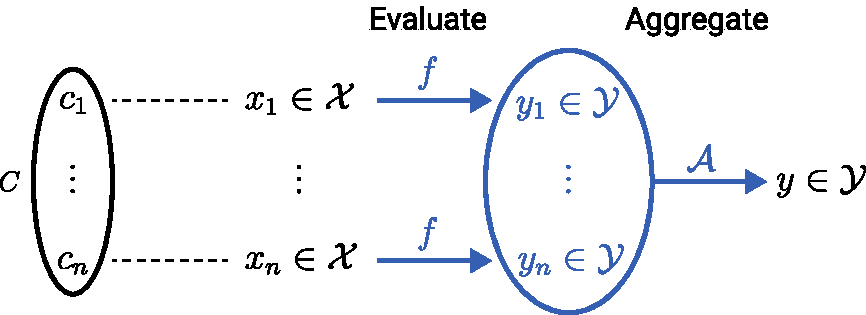
\includegraphics[width=0.7\linewidth]{gfx/related-work/lta-overview.pdf}
	\caption{Overview of the structure of LTA for multiset compositions.}\label{fig:related:lta-overview}
\end{figure}
Overall \ac{lta} can be understood as the joint problem of learning the aggregation function $\mathcal{A}$ and the local score derivation function $f$.
Two main approaches to represent the aggregation function in \ac{lta} problems have been explored.

\subsection{Uninorm-Aggregation}%
\label{sec:related:lta:uninorm}

The first approach uses \textit{uninorms}~\cite{Melnikov2016} to do so.
There the basic idea is to express composite scores as fuzzy truth assignments $y \in [0, 1]$.
Such a composite assignment $y$ is modeled as the result of a parameterized logical expression of constituent assignments $y_i \in [0, 1]$.
As the logical expression that thus effectively aggregates the constituents, a uninorm $U_{\lambda}$ is used.
Depending on the parameter $\lambda \in [0, 1]$, $U_{\lambda}$ combines a t-norm $T$ and a t-conorm $S$ which are continuous generalizations of logical conjunction and disjunction respectively.
One popular choice of norms are the so-called Łukasiewicz norms:
\begin{align}
	\text{t-norm } T(a, b) &\coloneqq \max \{ 0, a + b - 1 \}, \quad\text{t-conorm } S(a, b) \coloneqq \min \{ a + b, 1 \}, \nonumber \\
	\text{uninorm } U_\lambda(a, b) &\coloneqq \begin{cases}
		\lambda T\left(\frac{a}{\lambda}, \frac{b}{\lambda}\right) & \text{if } a, b \in [0, \lambda] \\
		\lambda + (1 - \lambda) S\left(\frac{a - \lambda}{1 - \lambda}, \frac{b - \lambda}{1 - \lambda}\right) & \text{if } a, b \in [\lambda, 1] \\
		\lambda \min \{ a, b \} & \text{else}
	\end{cases}
\end{align}
At the extreme points $(0, 0)$, $(0, 1)$, $(1, 0)$ and $(1, 1)$, $T$ and $S$ coincide with the Boolean operators $\land$ and $\lor$;
the values at all other points are interpolated as shown in \cref{fig:related:logic-norms}.
The uninorm $U_\lambda$ uses the conjunctive t-norm $T$ for values below the threshold $\lambda$ and the disjunctive t-conorm $S$ for values above the threshold.
$U_\lambda$ therefore smoothly interpolates between a conjunctive and disjunctive operator with the extreme points $U_1 = T$ and $U_0 = S$.
\begin{figure}[ht]
	\centering
	\begin{tikzpicture}
		\begin{axis}[
			title={t-norm $T$ ($\land$)},
			xlabel=$a$,
			ylabel=$b$,
			xlabel style={xshift=0.2cm, yshift=0.15cm},
			ylabel style={xshift=-0.2cm, yshift=0.15cm},
			tick label style={font=\scriptsize},
			width=0.33\textwidth,
			colormap = {bluered}{color(0cm) = (t_blue); color(1cm) = (t_red)}
		]
			\addplot3[
				mesh,
				samples=12,
				domain=0:1,
				domain y=0:1
			]{max(x + y - 1, 0)};
		\end{axis}
	\end{tikzpicture}
	\begin{tikzpicture}
		\begin{axis}[
			title={t-conorm $S$ ($\lor$)},
			xlabel=$a$,
			ylabel=$b$,
			xlabel style={xshift=0.2cm, yshift=0.15cm},
			ylabel style={xshift=-0.2cm, yshift=0.15cm},
			tick label style={font=\scriptsize},
			width=0.33\textwidth,
			colormap = {bluered}{color(0cm) = (t_blue); color(1cm) = (t_red)}
		]
			\addplot3[
				mesh,
				samples=12,
				domain=0:1,
				domain y=0:1
			]{min(x + y, 1)};
		\end{axis}
	\end{tikzpicture}
	\begin{tikzpicture}
		\begin{axis}[
			title={uninorm $U_{0.5}$ ($\land$/$\lor$)},
			xlabel=$a$,
			ylabel=$b$,
			xlabel style={xshift=0.2cm, yshift=0.15cm},
			ylabel style={xshift=-0.2cm, yshift=0.15cm},
			tick label style={font=\scriptsize},
			width=0.33\textwidth,
			colormap = {bluered}{color(0cm) = (t_blue); color(1cm) = (t_red)}
		]
			\addplot3[
				mesh,
				samples=12,
				domain=0:1,
				domain y=0:1
			]{(x <= 0.5 && y <= 0.5) * 0.5 * max(2 * (x + y) - 1, 0) + (x > 0.5 && y > 0.5) * (0.5 + 0.5 * min(2 * (x + y - 1), 1)) + (!(x <= 0.5 && y <= 0.5) && !(x > 0.5 && y > 0.5)) * min(x, y)};
		\end{axis}
	\end{tikzpicture}
	\caption{The Łukasiewicz norms and the corresponding uninorm for $\lambda = 0.5$.}\label{fig:related:logic-norms}
\end{figure}

Since t-norms and t-conorms are commutative and associative they can also be applied to non-empty sets of arbitrary size, i.e. $T(\ldblbrace y_1, \dots, y_n \rdblbrace) = T(y_1, T(\ldblbrace y_2, \dots, y_n \rdblbrace))$ with fixpoint $T(\ldblbrace y \rdblbrace) = y$.
Using this extension, a uninorm $U_\lambda$ can be applied to sets which turns it into a parameterized aggregation function $\mathcal{A}_\lambda: {[0, 1]}^* \to [0, 1]$.
In this simple model the \ac{lta} aggregation problem boils down to the optimization of $\lambda$.
The \ac{lta} disaggregation problem is solved by jointly optimizing a \acf{lm}, i.e.\ the constituent scores ${\ldblbrace y_i \in [0, 1] \rdblbrace}_{c_i \in \bm{c}}$ are described by $y_i = {\left( 1 + \exp(-\theta^\top x_i) \right)}^{-1}$.
Overall an \ac{lta} model is therefore described by the uninorm parameter $\lambda$ and the regression coefficients $\theta$.

\subsection{\acs*{owa}-Aggregation}%
\label{sec:related:lta:owa}

Recently \citet{Melnikov2019} have looked at an alternative class of aggregation functions.
Instead of using fuzzy logic to describe score aggregation, \ac{owa} operators were used.
\ac{owa} aggregators work by sorting the input scores and then weighting them based on their sort position, i.e.\ %
\begin{align}
	\mathcal{A}_{\lambda}(y_1, \dots, y_n) \coloneqq \sum_{i = 1}^n \lambda_i y_{\pi(i)},
\end{align}
where $\lambda \in \mathbb{R}^n$ is a weight vector with ${\|\lambda\|}_1 = 1$ and $\pi: [n] \to [n]$ is a sorting permutation of the input scores with $[n] \coloneqq \{ 1, \dots, n \}$ and $y_i < y_j \Rightarrow \pi(i) < \pi(j)$. % chktex 21
Depending on the choice of the vector $\lambda$, the \ac{owa} function $\mathcal{A}_\lambda$ can express common aggregation functions like
$\min$ (if $\lambda = (1, 0, \dots, 0)$),
$\max$ (if $\lambda = (0, \dots, 0, 1)$)
or the arithmetic mean (if $\lambda = \left(\frac{1}{n}, \dots, \frac{1}{n}\right)$).

To deal with varying composition sizes $n$, the weights $\lambda_1, \dots, \lambda_n$ can however not be statically assigned.
Instead they are interpolated using a so-called \ac{bum} function $q: [0, 1] \to [0, 1]$.
It takes constituent positions that are normalized to the unit interval, i.e.\ $\frac{i}{n} \in [0, 1]$.
The \ac{bum} function $q$ is then used to interpolate a weight for any normalized sort position via $\lambda_i \coloneqq q\left(\frac{i}{n}\right) - q\left(\frac{i - 1}{n}\right)$.
Because $q$ is monotone with $q(0) = 0$ and $q(1) = 1$, it always holds that ${\|\lambda\|}_1 = q(1) - q(0) = 1$. % chktex 21
Using this model, the aggregation problem boils down to optimizing the shape of $q$.

\begin{figure}[ht]
	\centering
	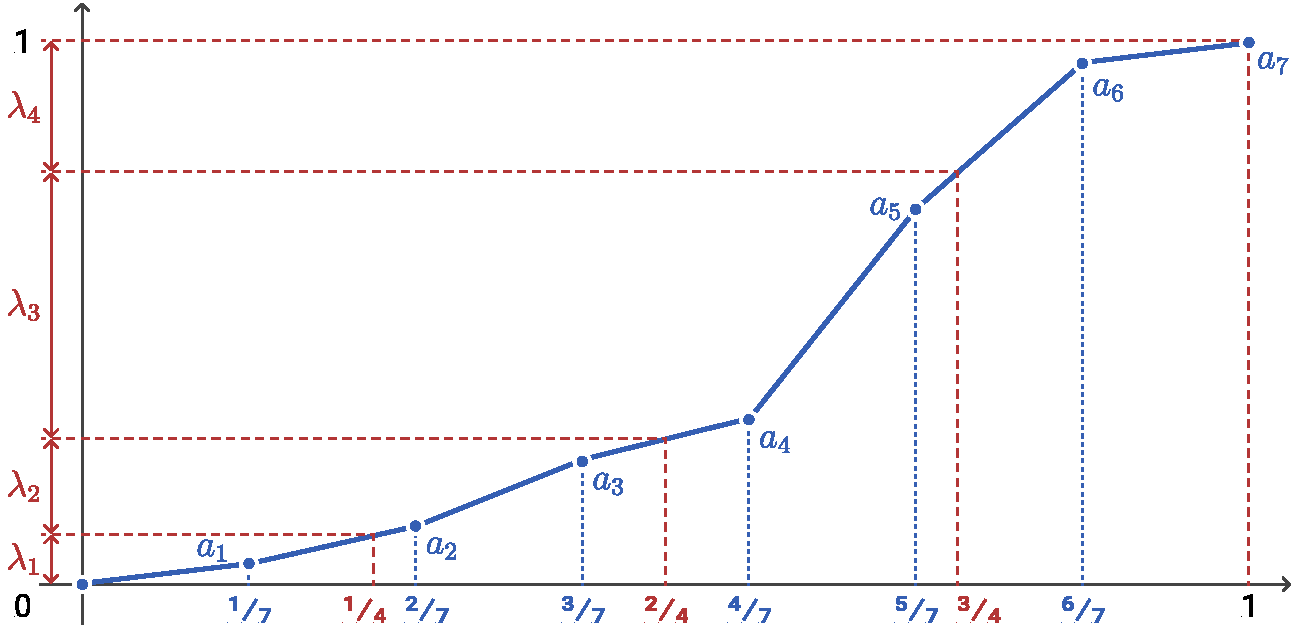
\includegraphics[width=0.75\linewidth]{gfx/related-work/bum.pdf}
	\caption[Illustration of how a \ac{bum} function is described as a linear spline and its relation to the \ac{owa} weights.]{
		Illustration of how \textcolor{t_blue}{$a$} describes \textcolor{t_blue}{$q$} and its relation to \textcolor{t_red}{$\lambda$} ($n = 4$, $m = 7$).
	}\label{fig:related:bum}
\end{figure}
In the \ac{owa} approach the \ac{bum} function $q$ is modeled as a piecewise linear spline.
This spline is described by $m+1$ points ${\left\{ \left( \frac{j}{m}, a_j \right) \right\}}_{j = 0}^{m}$, the so-called knots of the spline. % chktex 21
The curve of $q$ is obtained by linearly interpolating between neighboring knots as shown in \cref{fig:related:bum}.
If $0 = a_0 \leq a_1 \leq \cdots \leq a_m = 1$, $q$ is a \ac{bum} function.
The \ac{lta} aggregation problem is therefore solved by optimizing $a \in \mathbb{R}^{m + 1}$ under this constraint.
The disaggregation problem is tackled by adding the scores $y_1, \dots, y_M \in \mathbb{R}$ to the learnable parameters of the model where $M$ is assumed to be the finite number of constituents.
Currently the \ac{owa} approach requires all possible constituents to be part of the training dataset since it does not consider constituent features $x_i \in \mathcal{X}$ to predict the scores of previously unseen constituents.

\section{Graph Characterization}%
\label{sec:related:character}

\begin{defn}
	A graph $G \coloneqq (\mathcal{V}_G, \mathcal{E}_G)$ consists of a finite set of vertices $v_i \in \mathcal{V}_G$ and a set of edges $e_{ij} = (v_i, v_j) \in \mathcal{E}_G \subseteq \mathcal{V}_G^2$.
	Optionally discrete vertex labels $l_G[v_i] \in L_{\mathcal{V}}$ or edge labels $l_G[e_{ij}] \in L_{\mathcal{E}}$ may be associated with all vertices $v_i \in \mathcal{V}_G$ and edges $e_{ij}\in \mathcal{E}_G$ respectively.
	Also continuous feature vectors $x_G[v_{i}] \in \mathcal{X}_{\mathcal{V}}$, $x_G[e_{ij}] \in \mathcal{X}_{\mathcal{E}}$ may be given.
	If $\mathcal{X}_{\mathcal{E}} = \mathbb{R}$, $x_G[e_{ij}]$ can be interpreted as an edge weight of $e_{ij}$.

	In this thesis all graphs $G$ are assumed to be undirected if not explicitly stated otherwise, i.e.\ ${e_{ij} \in \mathcal{E}_G} \leftrightarrow\allowbreak {e_{ji} \in \mathcal{E}_G} \allowbreak\land l_G[e_{ij}] = l_G[e_{ji}] \allowbreak\land x_G[e_{ij}] = x_G[e_{ji}]$.
	We denote the set of all undirected graphs as $\mathcal{G}$.
	Additionally we denote $G[S] \coloneqq (S, \mathcal{E}_G \cap S^2)$ as the subgraph of $G$ induced by $S \subseteq \mathcal{V}_G$.
\end{defn}
To classify or score a graph, it first needs to be characterized by a set of relevant properties.
The most strict characterization of a graph is its so-called \textit{isomorphism class}.
It uniquely identifies a graph but lacks any notion of similarity between non-identical graphs.
We will begin with a brief definition of this strict isomorphism-based graph characterization.
Then two less strict characterization approaches are described; the so called \acl{wl} coloring and the notion of graph spectra.
They are the theoretical foundation of many current \ac{gcr} methods.

\subsection{The Graph Isomorphism Problem}%
\label{sec:related:character:iso}

In order to process a graph $G$ of size $n = |\mathcal{V}_G|$, one is forced to choose some encoding, e.g.\ an adjacency matrix $A \in {\{0, 1\}}^{n \times n}$.
Such an encoding introduces a vertex ordering $v_1, \dots, v_n$ that does not carry any semantic meaning.
Consequently there are $n!$ equivalent encodings of $G$. % chktex 40
To represent those encodings we introduce the notion of ordered induced subgraphs.
\begin{defn}\label{defn:related:ordered-subgraph}
	For all vertex $k$-tuples $v = (v_1, \dots, v_k) \in \mathcal{V}_G^k$ let $\hat{v} = \{ v_i\, |\, i \in [k] \}$.
	Then $G[v] \coloneqq (\hat{v}, \mathcal{E}_G \cap \hat{v}^2, v)$ is called the ordered subgraph of $G$ induced by $v$.
	If $\hat{v} = \mathcal{V}_G$ and $k = |\mathcal{V}_G|$, we call $v$ an ordering of $G$ and $G[v]$ an encoding of $G$.
\end{defn}
\begin{defn}\label{defn:related:ordered-subgraph-equivalence}
	Two ordered induced subgraphs $G[v]$ and $H[w]$ with $(v_1, \dots, v_k) \in \mathcal{V}_G^k$ and $(w_1, \dots, w_k) \in \mathcal{V}_H^k$ are \textit{equivalent} ($G[v] \equiv H[w]$) iff.\
	\begin{align*}
		&\quad\forall i, j \in [k]: (v_i, v_j) \in \mathcal{E}_G \leftrightarrow (w_i, w_j) \in \mathcal{E}_H \\
		&\, \begin{aligned}
			\land&\ \forall i, j \in [k]: l_G[v_i, v_j] = l_H[w_i, w_j] &\land&\ \forall i \in [k]: l_G[v_i] = l_H[w_i] \\
			\land&\ \forall i, j \in [k]: x_G[v_i, v_j] = x_H[w_i, w_j] &\land&\ \forall i \in [k]: x_G[v_i] = x_H[w_i]\text{.}
		\end{aligned}
	\end{align*}
	Using this notion of equivalence, we call $[G[v]] \coloneqq \{ G[w]\, |\, G[w] \equiv G[v] \land w \in \mathcal{V}_G^{*} \}$ the ordered subgraph equivalence class of $G[v]$.
\end{defn}
\begin{defn}
	Two graphs $G$ and $H$ are \textit{isomorphic} ($G \simeq H$) iff.\ there are equivalent encodings $G[v] \equiv H[w]$ of them.
	Consequently $[G] \coloneqq \{ H\, |\, H \simeq G \}$ is called the isomorphism class of $G$.
\end{defn}
The goal of the \ac{gi} problem is to check whether $G \simeq H$ for two arbitrary graphs.
Even though there is no known universal algorithm in $P$ that solves \ac{gi}, \citet{Babai1980} showed that almost all graphs can be trivially distinguished in linear time.
More recently \citet{Babai2015} also presented a quasipolynomial upper time bound for the remaining hard \ac{gi} instances.
For all practical purposes, \ac{gi} can therefore be solved efficiently; e.g.\ via the \texttt{nauty} program~\cite{McKay}\cite{McKay2013}.
One important subroutine in most \ac{gi} checkers is the \acl{wl} algorithm which will be described next.

\subsection{\acl{wl} Graph Colorings}%
\label{sec:related:character:wl}

The \acf{wl} algorithm~\cite{Weisfeiler1968}\cite{Cai1992} characterizes a graph $G$ by assigning discrete labels $c \in \mathcal{C}$, called \textit{colors}, to vertex $k$-tuples $(v_1, \dots, v_k) \in \mathcal{V}_G^k$, where $k \in \mathbb{N}$ is the freely choosable \textit{\ac{wl}-dimension}.
A mapping $\chi_{G, k}: \mathcal{V}_G^k \to \mathcal{C}$ is called a \textit{$k$-coloring} of $G$.
\begin{defn}
	A coloring $\chi'$ \textit{refines} $\chi$ ($\chi' \preceq \chi$) iff.\ $\forall a, b \in \mathcal{V}_G^k: \chi(a) \neq \chi(b) \rightarrow \chi'(a) \neq \chi'(b)$, i.e.\ $\chi'$ distinguishes at least those tuples that are distinguished by $\chi$.
\end{defn}
\begin{defn}
	Two colorings $\chi$ and $\chi'$ are \textit{equivalent} ($\chi \equiv \chi'$) iff.\ $\chi \preceq \chi' \land \chi' \preceq \chi$, i.e.\ $\chi$ is identical to $\chi'$ up to color substitutions.
\end{defn}
The $k$-dimensional \ac{wl} algorithm ($k$-\acs{wl}) works by iteratively refining $k$-colorings $\chi_{G, k}^{(0)} \succeq \chi_{G, k}^{(1)} \succeq \dots$ of a given graph $G$ until the convergence criterion $\chi_{G, k}^{(i)} \equiv \chi_{G, k}^{(i+1)}$ is satisfied.
We denote the final, maximally refined $k$-\acs{wl} coloring with $\chi^{*}_{G, k}$.
\begin{defn}
	The color distribution $\mathit{dist}_{\chi_{G, k}}: \mathcal{C} \to \mathbb{N}$ of a $k$-coloring $\chi_{G, k}$ counts each color $c \in \mathcal{C}$ in the coloring, i.e.\ $\mathit{dist}_{\chi_{G, k}}(c) \coloneqq \left|\left\{ v \in \mathcal{V}_G^k\, |\, \chi_{G, k}(v) = c \right\}\right|$. % chktex 21
\end{defn}
\begin{defn}\label{defn:related:wl-distinguishable}
	Two graphs $G$ and $H$ are are $k$-\acs{wl} \textit{distinguishable} ($G \mathrel{{\not\simeq}_k} H$) iff.\ there exists a color $c \in \mathcal{C}$ s.t.\ $\mathit{dist}_{\chi^{*}_{G, k}}(c) \neq \mathit{dist}_{\chi^{*}_{H, k}}(c)$.
\end{defn}
As we will see, the way in which \ac{wl} colorings are refined is vertex order invariant;
thus any difference in the final coloring of two graphs always implies the non-isomorphism of the colored graphs, i.e.\ $G \mathrel{{\not\simeq}_k} H \implies G \not\simeq H$.
The opposite does however not necessarily hold;
two $k$-\acs{wl} indistinguishable graphs are not always isomorphic, i.e.\ $\exists\, G, H: G \mathrel{{\simeq}_k} H \land G \not\simeq H$. % chktex 21

In addition to the binary aspect of \ac{wl} distinguishability and its relation to the \ac{gi} problem, \ac{wl} colorings are also useful for more fuzzy graph similarity comparisons as we will see in \cref{sec:related:gcr:kernel} when we look at graph kernels.
Before that however, the details of \ac{wl} color refinement strategy have to be described.
We begin with the color refinement algorithm for the most simple case of $k = 1$.
Then the definitions and intuitions from the 1-dimensional case are extended to its higher-dimensional generalization.
Lastly we will discuss the discriminative power of the \acs{wl} algorithm and its relation to the \acs{wl}-dimension $k$.

\subsubsection{The 1-dimensional \acs{wl} algorithm}
In the 1-dimensional \ac{wl} algorithm, a color is assigned to each vertex of a graph.
If the vertices $v \in \mathcal{V}_G$ of the input graph $G$ are labeled, those labels $l_G[v] \in L_{\mathcal{V}} \subseteq \mathcal{C}$ can be used as the initial graph coloring $\chi_{G,1}^{(0)}(v) \coloneqq l_G[v]$.
Since \ac{wl} colors are inherently discrete, continuous vertex feature vectors $x_G[v]$ are not considered here.
For unlabeled graphs a constant coloring is used, e.g.\ $\forall v \in \mathcal{V}_G: \chi_{G,1}^{(0)}(v) = \textcolor{t_blue}{\texttt{A}}$ for some initial color $\textcolor{t_blue}{\texttt{A}} \in \mathcal{C}$. % chktex 25
In each iteration of the 1-\acs{wl} color refinement algorithm, the following neighborhood aggregation scheme is used to compute a new color for all vertices:
\begin{defn}\label{defn:related:wl1-refine}
	$\chi_{G,1}^{(i+1)}(v) \coloneqq h\left(\chi_{G,1}^{(i)}(v), \ldblbrace \chi_{G,1}^{(i)}(u)\, |\, u \in \Gamma_{G}(v) \rdblbrace\right)$,
	with $\Gamma_G(v)$ denoting the set of adjacent vertices of $v \in \mathcal{V}_G$ and $h: \mathcal{C}^* \to \mathcal{C}$ denoting a perfect hash function that assigns a unique color to each finite combination of colors.
\end{defn}
In practice the hash function $h$ is usually defined lazily by using $\mathcal{C} = \mathbb{N}$ and enumerating color combinations in whichever order they are hashed s.t.\ a new color is introduced every time a previously unseen color combination appears at runtime.
This is illustrated in \cref{fig:related:wl1-refine}.
\begin{figure}[ht]
	\centering
	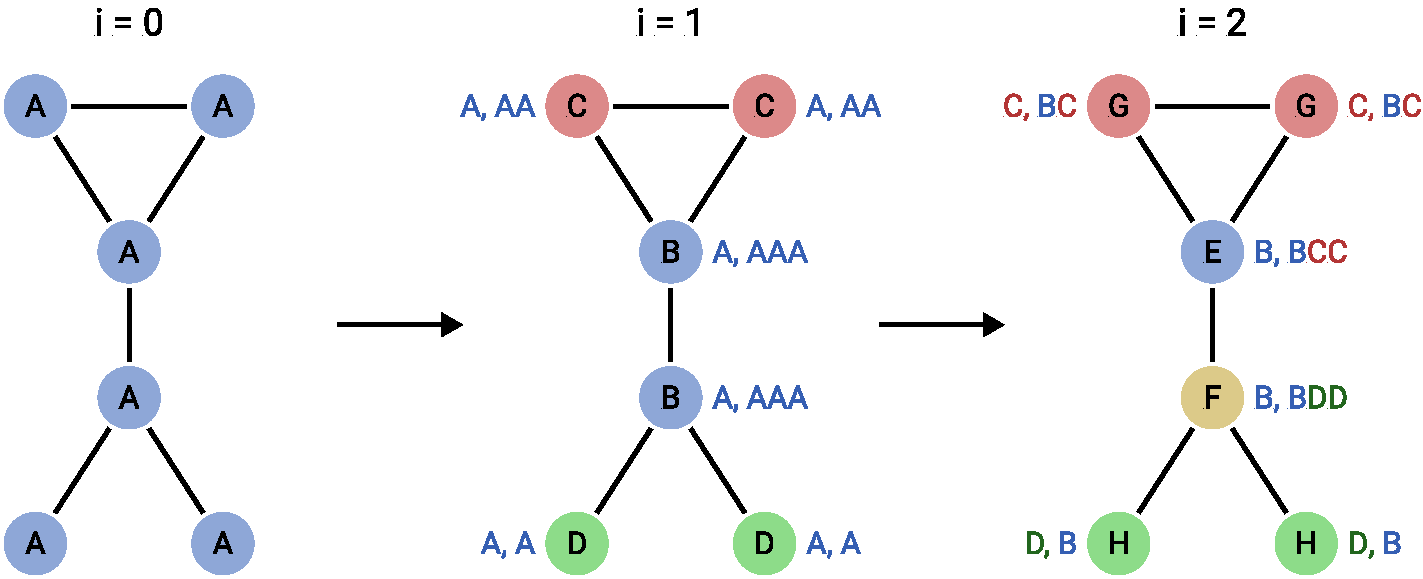
\includegraphics[width=0.72\linewidth]{gfx/related-work/wl1-refine.pdf}
	\caption[Example 1-WL color refinement steps.]{
		Example 1-WL color refinement steps.
		After two iterations the coloring stabilizes.
		Each vertex $v$ is labeled with its current color and has its previous color and the colors of the hashed neighbors $\Gamma_G(v)$ written next to it (see \cref{defn:related:wl1-refine}).
	}\label{fig:related:wl1-refine}
\end{figure}

\subsubsection{The $k$-dimensional \acs{wl} algorithm}
As we just saw, the 1-\acs{wl} algorithm iteratively refines colorings of single vertices.
While the obtained colorings differ for most non-isomorphic graphs $G \not\simeq H$, 1-\acs{wl} does not generally solve the \ac{gi} problem as illustrated in \cref{fig:related:wl1-problem}.
\begin{figure}[ht]
	\centering
	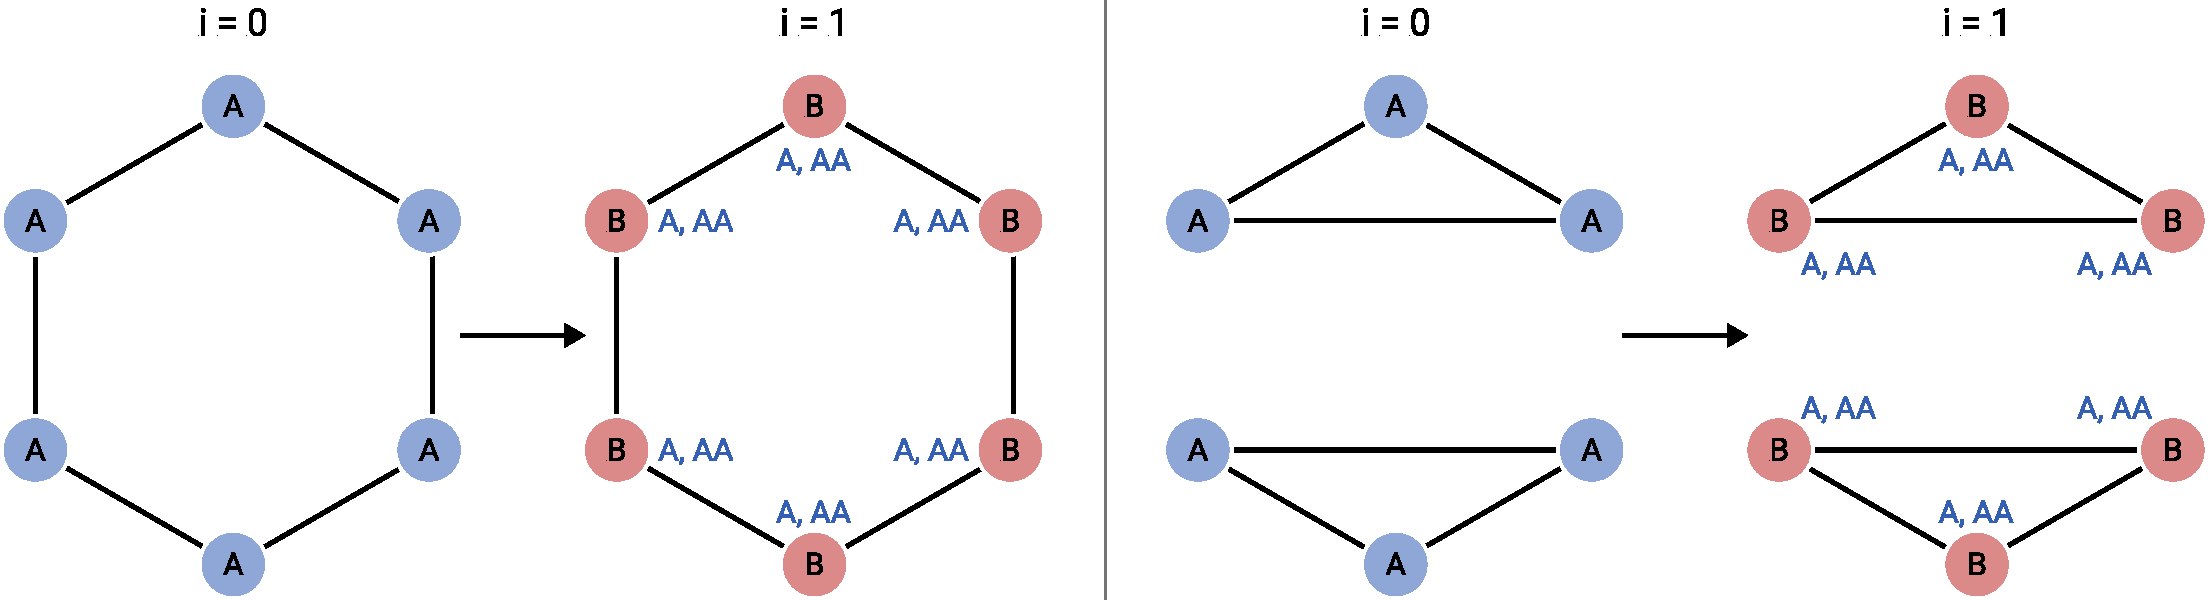
\includegraphics[width=\linewidth]{gfx/related-work/wl1-problem.pdf}
	\caption[Two simple non-isomorphic graphs that are indistinguishable by 1-\acs{wl}.]{
		Two simple non-isomorphic graphs that are indistinguishable by 1-\acs{wl}.
	}\label{fig:related:wl1-problem}
\end{figure}
By extending \ac{wl} to higher dimensions, such 1-\acs{wl} indistinguishable cases can however be handled.
Analogous to the 1-dimensional \cref{defn:related:wl1-refine}, the $k$-dimensional color refinement step is defined by
\begin{defn}\label{defn:related:wlk-refine}
	$\begin{aligned}[t]
		\chi_{G,k}^{(i+1)}(v) \coloneqq h\left(\chi_{G,k}^{(i)}(v), \ldblbrace (\chi_{G,k}^{(i)}(v[u/1]), \dots, \chi_{G,k}^{(i)}(v[u/k]))\, |\, u \in \mathcal{V}_G \rdblbrace\right)\\
		\text{with } v = (v_1, \dots, v_k) \in \mathcal{V}_G^k,\quad v[u/j] \coloneqq (v_1, \dots, v_{j-1}, u, v_{j+1}, \dots, v_k) \text{.}
	\end{aligned}$
\end{defn}
In 1-\acs{wl} a vertex color is refined by combining the colors of neighboring vertices.
In $k$-\acs{wl} the color of a $k$-tuple $v \in \mathcal{V}_G^k$ is refined by combining the colors of its neighborhood which is defined as the set of all $k$-tuples in which at most one vertex differs from $v$.
Note that each vertex $k$-tuple has one neighbor for each $u \in \mathcal{V}_G$, each of which is a $k$-tuple of vertex $k$-tuples.
This more abstract notion of neighborhood is illustrated in \cref{fig:related:wl-neighbors}.
\begin{figure}[ht]
	\centering
	\begin{subfigure}{0.33\textwidth}
		\centering
		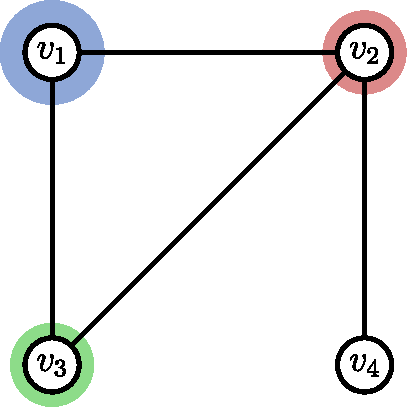
\includegraphics[width=0.8\linewidth]{gfx/related-work/wl1-neighbors.pdf}
		\subcaption{1-WL $v_1$ neighbors}\label{fig:related:wl-neighbors:1}
	\end{subfigure}%
	\begin{subfigure}{0.33\textwidth}
		\centering
		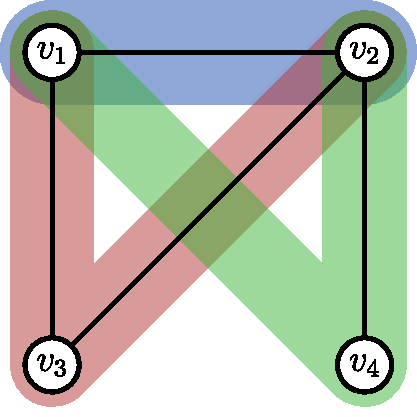
\includegraphics[width=0.8\linewidth]{gfx/related-work/wl2-neighbors.pdf}
		\subcaption{2-WL $(v_1, v_2)$ neighbors}\label{fig:related:wl-neighbors:2}
	\end{subfigure}%
	\begin{subfigure}{0.33\textwidth}
		\centering
		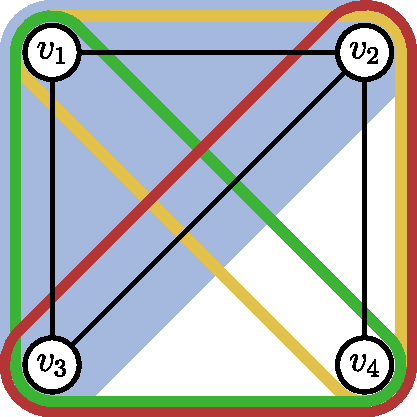
\includegraphics[width=0.8\linewidth]{gfx/related-work/wl3-neighbors.pdf}
		\subcaption{3-WL $(v_1, v_2, v_3)$ neighbors}\label{fig:related:wl-neighbors:3}
	\end{subfigure}
	\caption[\ac{wl} neighborhoods for different values of $k$.]{
		Tuple neighborhoods for different values of $k$.
		The vertices highlighted in \textcolor{t_blue}{blue} form the root tuple $v \in \mathcal{V}_G^k$ whose neighbors are shown;
		for simplicity neighbors with $u \in v$ are left out (see~\cref{defn:related:wlk-refine}).
		Each neighbor is highlighted with a different color, except for 3-WL where the \textcolor{t_red}{red}, \textcolor{t_green}{green} and \textcolor{t_darkyellow}{yellow} triples actually form the single neighbor for $u = v_4$.
	}\label{fig:related:wl-neighbors}
\end{figure}
For $k = 2$ this means that each potential edge $(v, w) \in \mathcal{V}_G^2$ has all possible paths of length $2$ from $v$ to $w$ as its neighbors (see~\cref{fig:related:wl-neighbors:2}).
Also note that, even though $k$-\acs{wl} refines $k$-tuple colors, lower-dimensional structures still get their own colors since a tuple does not have to consist of distinct vertices, i.e.\ in $k$-\acs{wl} the color of a single vertex $v \in \mathcal{V}_G$ is described by $\chi^{*}_{G, k}(s)$ for $s = (v, \dots, v) \in \mathcal{V}_G^k$.

Let us now look at how the tuple colors are initialized.
For this we use the ordered subgraph equivalence classes $[G[v]]$ (see~\cref{defn:related:ordered-subgraph-equivalence}) which determine the initial color $\chi_{G,k}^{(0)}(v)$ of each $k$-tuple $v$.
For $k = 1$ the equivalence class of a single vertex $v$ directly corresponds to its label $l_G[v]$.
More generally for $k > 1$ this means that
\begin{align}
	\chi_{G,k}^{(0)}(v) = \chi_{G,k}^{(0)}(w) \iff G[v] \equiv G[w] \text{.} \label{eq:related:wlk-init}
\end{align}
Note that there is a fundamental difference in how the adjacency information encoded in $\mathcal{E}_G$ is used in 1-\acs{wl} vs.\ $k$-\acs{wl}:
In 1-\acs{wl} a vertex coloring by itself cannot encode adjacency which is why this information is explicitly incorporated in each refinement step via $\Gamma_G$ (see~\cref{defn:related:wl1-refine}).
In $k$-\acs{wl} on the other hand each pair of vertices $(v, u) \in \mathcal{V}_G^2$ appears in at least one $k$-tuple (assuming $k \geq 2$) and therefore has at least one color which can implicitly encode the adjacency information.
Edges and non-edges are colored differently in the initial coloring since $G[(v, u)] \not\equiv G[(w, u)]$ if $(v, u) \in \mathcal{E}_G$ but $(w, u) \notin \mathcal{E}_G$;
thus no explicit adjacency information is needed in the $k$-\acs{wl} color refinement step in \cref{defn:related:wlk-refine}.

\subsubsection{Discriminative Power of \acs{wl}}
Now we will look at the types of graphs that can be distinguished by \acs{wl} in relation to the \acs{wl}-dimension $k$.
\begin{lem}\label{lem:related:wl-lower}
	$G \mathrel{\not\simeq_k} H \implies G \mathrel{\not\simeq_{k+1}} H$ ($(k+1)$-\acs{wl} is at least as powerful as $k$-\acs{wl}).
\end{lem}
\begin{hproof}
	All $k$-tuples can be mapped to $(k+1)$-tuples via $\varphi(v_1, \dots, v_k) \coloneqq (v_1, \dots,\allowbreak v_k, v_k)$.
	For each neighbor $(v[u/1], \dots,\allowbreak v[u/k])$ of $v$, there is a corresponding neighbor $(\varphi(v[u/1]), \dots \varphi(v[u/k]), \varphi(v[u/k]))$ of $\varphi(v)$.
	Using \cref{eq:related:wlk-init} (for $i = 0$) and \cref{defn:related:wlk-refine} (for $i > 0$) it follows that $\forall v, w \in \mathcal{V}_G^k: \chi_{G, k}^{(i)}(v) \neq \chi_{G, k}^{(i)}(w) \rightarrow \chi_{G, k+1}^{(i)}(\varphi(v)) \neq \chi_{G, k+1}^{(i)}(\varphi(w))$.
	The lemma then follows by \cref{defn:related:wl-distinguishable}.
\end{hproof}
\begin{prop}[see~\citet{Immerman1990}]\label{prop:related:wl-upper}
	For all $k \in \mathbb{N}$ there are non-isomorphic graphs $G \not\simeq H$ of size $\mathcal{O}(k)$ with $G \mathrel{\simeq_k} H$.
\end{prop}
\begin{cor}\label{cor:related:wl-monotonous}
	The discriminative power of $k$-\acs{wl} grows monotonously with $k$ and never converges, i.e.\ for all $k \in \mathbb{N}$ there is an $l \in \mathbb{N}$ s.t.\ the set of $k$-\ac{wl} distinguishable graphs is a proper subset of the $(k+l)$-\ac{wl} distinguishable graphs.
\end{cor}
\begin{hproof}
	Note that $k$-\acs{wl} trivially solves the \ac{gi} problem for all graphs of size $\leq k$ via the initial coloring (see~\cref{eq:related:wlk-init}).
	Using \cref{lem:related:wl-lower} and \cref{prop:related:wl-upper} the corollary directly follows.
\end{hproof}
\begin{figure}[ht]
	\centering
	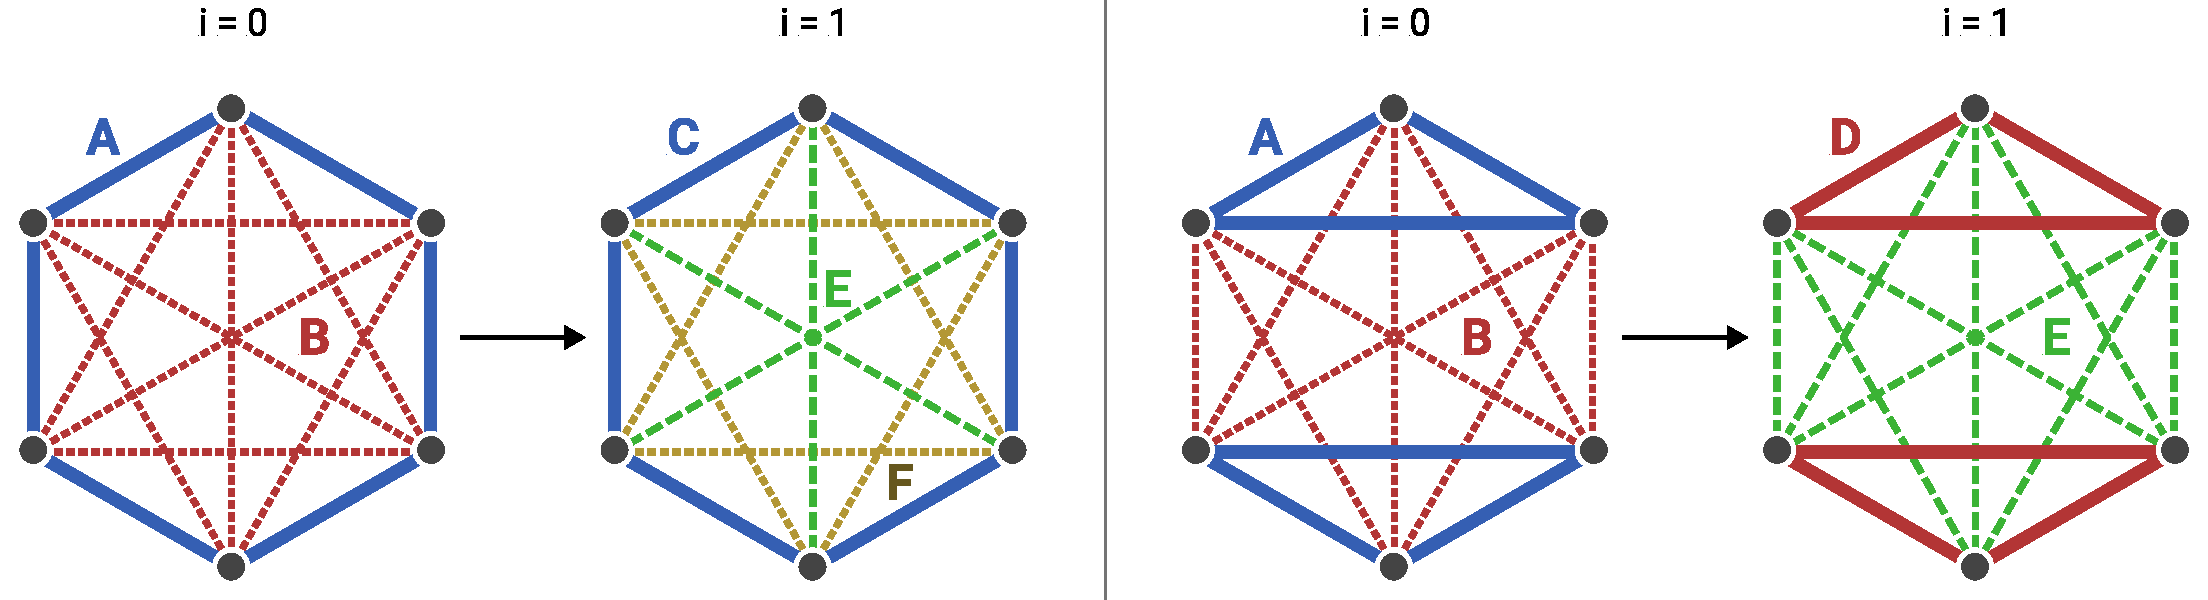
\includegraphics[width=\linewidth]{gfx/related-work/wl2-problem-solution.pdf}
	\caption{
		Two non-isomorphic graphs with $G \mathrel{\simeq_1} H$ and $G \mathrel{\not\simeq_2} H$.
	}\label{fig:related:wl2-problem-solution}
\end{figure}
\Cref{fig:related:wl2-problem-solution} illustrates \cref{cor:related:wl-monotonous} by showing how 2-WL is able to distinguish the two 1-WL indistinguishable graphs from \cref{fig:related:wl1-problem}.
Since the time complexity of $k$-\acs{wl} grows exponentially with $k$~\cite[cor.~1.9.7]{Immerman1990}, it does not provide an efficient universal solution to \ac{gi}.
However it turns out that almost all graphs are \ac{wl} distinguishable even for a small constant $k$.

For $k = 1$ \citet{Babai1980} have shown that two randomly selected non-isomorphic graphs $G \not\simeq H$ of size $n$ are 1-\acs{wl} indistinguishable with probability $n^{-\nicefrac{1}{7}}$.
Thus 1-\acs{wl} is already able to distinguish most graphs; it fails however to distinguish any pair of unlabeled $d$-regular graphs of the same size~\cite[cor.~1.8.5]{Immerman1990}.
\begin{defn}
	A graph $G$ is called $d$-regular ($\mathit{rg}_d(G)$) iff.\ $\forall v \in \mathcal{V}_G: {|\Gamma_G(v)|} = d$.
\end{defn}
We have already seen this in \cref{fig:related:wl1-problem} since the ``six-cycle'' and the ``two-triangles'' graphs are in fact both 2-regular and of size 6.
This restriction alone is typically not an issue in the context of \ac{gcr} though, as molecular structures or social interaction graphs for example are rarely perfectly regular.
A more relevant restriction of 1-\acs{wl} is the fact that it is unable to detect cycles of length $m \geq 3$.
\begin{defn}\label{defn:related:wl-compute}
	$k$-\acs{wl} computes a function $f: \mathcal{G} \to Y$ iff.\ that function can be expressed as $f(G) = g(\mathit{dist}_{\chi_{G, k}^{*}})$ via some function $g: (\mathcal{C} \to \mathbb{N}) \to Y$.
\end{defn}
\begin{defn}\label{defn:related:wl-count-detect}
	$k$-\acs{wl} counts a certain subgraph $S$ iff.\ it computes $\mathit{count}_S(G) \coloneqq \left|\{ \hat{v}\, |\, v \in \mathcal{V}_G^{*} \land G[v] \equiv S \}\right|$ (see~\cref{defn:related:ordered-subgraph}).
	Similarly $k$-\acs{wl} detects a subgraph $S$ iff.\ it computes $\mathit{contain}_S(G) \coloneqq \mathbbm{1}[\mathit{count}_S(G) > 0]$, with $\mathbbm{1}$ denoting the indicator function.
\end{defn}
To see why 1-\acs{wl} is unable to detect $m$-cycles in graphs, note that \cref{fig:related:wl1-problem} already contradicts the positive statement for $m = 3$;
this counterexample can be trivially generalized to all larger $m$ by replacing the ``six-cycle'' graph with a ``$(2m)$-cycle-graph'' graph and the ``two-triangles'' graph with a ``two-$m$-cycles'' graph which preserves the 2-regularity and therefore the 1-\acs{wl} indistinguishability.

This cycle-detection restriction of 1-\acs{wl} is relevant in practice because cycle counts are used in many domains to analyze graphs, e.g.\ triangle counts are commonly used in social network analysis to find interaction clusters~\cite{Newman2003}\cite{Welser2007} and the detection of 4-, 5- or 6-cycles is required to determine important chemical properties like the aromaticity of a molecule~\cite{Adamson1973}\cite{Kekule1866}.

If we increase the \acs{wl}-dimension to $k = 2$, the described 1-\acs{wl} restrictions no longer apply.
2-\acs{wl} is able to distinguish more than $1 - \mathcal{O}(\nicefrac{1}{n})$ of the regular $n$-vertex graphs~\cite[cor.~1.8.6]{Immerman1990} and can even count cycles.
\begin{prop}[see \citet{Fuerer2017} and \citet{Arvind2019}]\label{prop:related:wl2-cycle-count}
	2-\acs{wl} is able to count $m$-cycles for $m \leq 7$ but it cannot detect 8-cycles.
\end{prop}
\begin{hproof}
	Only the idea behind triangle and 4-cycle counting is outlined here to give an intuition for why \cref{prop:related:wl2-cycle-count} holds.
	Note that the 2-\acs{wl} neighbors of each edge $(v, w) \in \mathcal{E}_G$ correspond to all possible paths $(v, u, w)$ of length 2, i.e.\ all possible triangles.
	By \cref{defn:related:wlk-refine} there must thus be a color subset $C^{\triangle}_j \subseteq \mathcal{C}$ representing that an edge is involved in exactly $j$ triangles after one refinement step.
	2-\acs{wl} then trivially counts triangles by setting $g(\mathit{dist}_\chi) = \frac{1}{3} \sum_j j \sum_{c \in C^{\triangle}_j} \mathit{dist}_\chi(c)$ to satisfy \cref{defn:related:wl-compute}.
	Analogously for 4-cycles, let $C^{\square}_j \subseteq \mathcal{C}$ be the colors indicating a non-edge $(v, w) \notin \mathcal{E}_G$ with $j$ common vertex neighbors $u \in \Gamma_G(v) \cap \Gamma_G(w)$.
	The number of 4-cycles is then determined by the colors of the diagonals through them via $g(\mathit{dist}_\chi) = \frac{1}{2} \sum_{j \geq 2} \binom{j}{2} \sum_{c \in C^{\square}_j} \mathit{dist}_\chi(c)$.
	Using a similar but more involved combinatorial argument requiring multiple color refinement steps, 5-, 6- \& 7-cycle counting can be shown.
\end{hproof}
As we just saw, 2-\acs{wl} is significantly more powerful than 1-\acs{wl}.
By \cref{prop:related:wl-upper} there are of course still 2-\acs{wl} indistinguishable graphs;
among others those are the strongly regular graphs $\mathit{srg}_{n, d, \lambda, \mu}(G)$.
\begin{defn}
	$\begin{aligned}[t]
		\mathit{srg}_{n, d, \lambda, \mu}(G) \iff\ & {|\mathcal{V}_G|} = n \quad\land\quad \forall v \in \mathcal{V}_G: {|\Gamma_G(v)|} = d \\
		&\land \forall (v, w) \in \mathcal{E}_G: {|\Gamma_G(v) \cap \Gamma_G(w)|} = \lambda \\
		&\land \forall (v, w) \in \mathcal{V}_G^2 \setminus \mathcal{E}_G: {|\Gamma_G(v) \cap \Gamma_G(w)|} = \mu
	\end{aligned}$
\end{defn}
Generally this restriction of 2-\acs{wl} is not an issue since strongly regular graphs do not appear in typical \ac{gcr} datasets.
By going to $k = 3$, even some strongly regular graphs as well as all planar graphs can be distinguished though~\cite{Kiefer2017}.
Apart from that there are currently few results regarding the classes of distinguishable graphs and computable functions for even higher \ac{wl}-dimensions.

\subsection{Spectral Graph Theory}%
\label{sec:related:character:spectral}

An alternative perspective on graph characterization is provided by \textit{spectral graph theory}.
While \ac{wl} characterizes a graph via its color distribution $\mathit{dist}_{\chi_{G,k}^{*}}$, the spectral approach uses its so-called \textit{spectrum} $\lambda_G = (\lambda_{G, 1}, \dots, \lambda_{G, n}) \in \mathbb{R}^n$ where $n = |\mathcal{V}_G|$.
The key idea behind this is to interpret the adjacency matrix $A \in \mathbb{R}^{n \times n}$ of $G$ not simply as an encoding of the edges ($A_{i j} = \mathbbm{1}[(v_i, v_j) \in \mathcal{E}_G]$) but as a linear operator $A: (\mathcal{V}_G \to \mathbb{R}) \to (\mathcal{V}_G \to \mathbb{R})$ acting on the vector space of real-valued functions with a vertex domain.
This means that $A$ transforms so-called \textit{graph signals} $x: \mathcal{V}_G \to \mathbb{R}$ which are functions assigning \textit{signal strengths} to vertices.
By applying $Ax$ the signal strength $x[v_i]$ of each vertex is added to the signal strengths of its neighbors $\Gamma_G(v_i)$.
Using this functional perspective, one can characterize graphs via the \acf{ft}.
We will now see how this is done;
however since a comprehensive description of spectral graph theory would exceed the scope of this thesis, only a brief overview will be given.
For a more detailed introduction to the field we refer to \citet{Shuman2013}.

\paragraph{\ac{ft} on complex domains}
Let us begin by describing the \ac{ft} for the more common case of functions with complex domains\footnote{
	This description of the \ac{ft} naturally also includes functions with real domains.
	The complex case was chosen because it is more compact.
}.
All functions $f: \mathbb{C} \to \mathbb{C}$ can be interpreted as infinite-dimensional vectors $f = \int_{\mathbb{C}} f(t)\, b_t \dif t$ with $b_t: \mathbb{C} \to \mathbb{C}$ being a standard basis vector/function defined as $b_t(s) \coloneqq \begin{cases} 1 & \text{if } s = t \\[-6pt] 0 & \text{else} \end{cases}$. % chktex 21
The \acl{ft} $\hat{f}$ of $f$ corresponds to a change of basis from the standard basis vectors $b_t$ to the Fourier basis vectors $u_\xi(t) \coloneqq e^{2 \pi i \xi t}$, i.e.\ $f = \int_{\mathbb{C}} \hat{f}(t)\, u_\xi \dif \xi$.
The Fourier basis is characterized by the fact that it is an eigenbasis of the so-called \textit{Laplace operator} $\Delta$, i.e.\ $\Delta u_\xi = \lambda_\xi u_\xi$ with $\lambda_\xi$ being the eigenvalue corresponding to $u_\xi$.
In the complex domain this Laplace operator $\Delta$ is effectively the same as the second-derivative $\frac{\dif^2}{\dif t^2}$.
Thus it is easy to see that indeed $\Delta u_\xi = \frac{\dif^2}{\dif t^2} u_\xi = \lambda_\xi u_\xi$ for $\lambda_\xi = -{(2 \pi \xi)}^2$.
Note that the complex exponentials $u_\xi$ are the only eigenbasis of $\Delta$ on the complex plane $\mathbb{C}$.
This allows us to interpret the eigenvectors $u_\xi$ and their corresponding eigenvalues $\lambda_\xi$ as a characterization of the complex plane.

\paragraph{\ac{ft} on vertex domains}
Similar to how the eigenvectors and eigenvalues of the complex Laplacian $\frac{\dif^2}{\dif t^2}$ characterize $\mathbb{C}$, we can characterize a graph $G$ by the eigenvectors and eigenvalues of the so-called \textit{combinatorial graph Laplacian} $L$.
\begin{defn}
	The combinatorial graph Laplacian $L$ of a graph $G$ is defined as
	\begin{align*}
		L \coloneqq D - A\quad\text{with the degree matrix } D \coloneqq {
			\renewcommand*{\arraystretch}{0.5}
			\begin{pmatrix}
				d_1 & & \\
				& \ddots & \\
				& & d_n
			\end{pmatrix}
		}, d_i \coloneqq |\Gamma_G(v_i)| \text{.}
	\end{align*}
\end{defn}

\section{Graph Classification and Regression}%
\label{sec:related:gcr}

The existing approaches to tackle the \ac{gcr} problem can be categorized into three main families:
\begin{enumerate*}
	\item Explicit graph embeddings,
	\item graph kernels and
	\item graph neural networks
\end{enumerate*}.
We will now look at the characteristics of those families and give a brief overview of specific methods.

\subsection{Explicit Graph Embeddings}%
\label{sec:related:gcr:embed}

The basic idea of explicit graph embedding approaches is to map a graph $G \in \mathbb{G}$ to some vector in a finite vector space $\mathcal{X} = \mathbb{R}^d$.
A function $f: \mathbb{G} \to \mathcal{X}$ is called a \textit{graph embedding function}.
By embedding a graph into $\mathcal{X}$, any classification or regression algorithm that works with vectors can then be applied to solve the \ac{gcr} problem.

The so-called vertex embedding problem is closely related to the graph embedding problem.
As the name suggests, a \textit{vertex embedding function} $f_G: V \to \mathcal{X}$ maps all vertices $v \in V$ of a graph $G$ into $\mathcal{X}$.
The embedding vector $f_G(v)$ ideally encodes relevant information about a vertex and its structural position in $G$.
It can be used to solve the vertex classification and regression problem via arbitrary \ac{ml} methods for vectors.
We will now look at two main families of explicit graph and vertex embedding approaches.

\subsubsection{Fingerprint Embeddings}

The first works on graph embeddings were motivated by the study of chemical structures~\cite{Adamson1973}\cite{Willett1986}.
There a molecule can be interpreted as a labeled graph for which the \ac{gcr} problem corresponds to the prediction of some chemical property, e.g.\ toxicity or solubility.
So-called \textit{fingerprint embeddings} try to match a fixed set of subgraphs $S_1, \dots, S_d$ to the input graph.
The embedding of a graph $G$ is a binary vector $f(G) = x \in {\{0, 1\}}^d$ with $x_i \coloneqq \mathit{contain}_{S_i}(G)$ (see~\cref{defn:related:wl-count-detect}).
This simple approach usually requires a careful choice of subgraphs but can still be competitive with the other more recent approaches we will look at in the following sections.
Fingerprint embeddings are for example used in multiple state-of-the-art toxicity prediction tools like RASAR~\cite{Luechtefeld2018}\cite{ToxTrack}, ProTox~\cite{Drwal2014}\cite{Banerjee2018}\cite{ProTox} or the \ac{toxTest}~\cite{TEST}.

\subsubsection{Skip-gram inspired Embeddings}

Skip-gram embeddings were introduced by \citeauthor{Mikolov2013} as part of the well-known \texttt{word2vec}~\cite{Mikolov2013} word embedding method from \ac{nlp}.
While a fingerprint embedding explicitly assigns an interpretation to each embedding dimension (i.e.\ to each standard basis vector), a skip-gram embedding only optimizes the distance between embedding vectors based on the similarity of the embedded instances without providing an interpretation of the embedding dimensions.

\paragraph{word2vec}
Let us first look at the \texttt{word2vec} skip-gram method.
It gets a sequence of words $(w_0, \dots, w_n)$ as input and outputs embedding vectors $f(w_0), \dots, f(w_n) \in \mathbb{R}^d$.
To do this the context $C_k(w_i) = \{ w_{i-k}, \dots, w_{i + k} \}$ is computed for all words where $w_i$ is the so-called \textit{context root}.
The word contexts are then used to optimize the following log-likelihood objective:
\begin{gather}
	\max_{f, f_C} \sum_{i = 1}^n \log P(C_k(w_i) | w_i)\ =\ \max_{f, f_C} \sum_{i = 1}^n \smashoperator[r]{\sum_{w_j \in C_k(w_i)}}\, \left[ {f(w_i)}^\top f_C(w_j) - \log Z_{w_i} \right] \label{eq:related:gcr:embed:word2vec}\\
	\text{with } P(C_k(w_i) | w_i) \coloneqq \prod_{\mathclap{w_j \in C_k(w_i)}}\, \overbrace{\frac{\exp\left({f(w_i)}^\top f_C(w_j)\right)}{Z_{w_i}}}^{P(w_j | w_i)}
	\text{ and } Z_{w_i} \coloneqq \sum_{j = 1}^n \exp\left({f(w_i)}^\top f_C(w_j)\right) \nonumber
\end{gather}
\texttt{word2vec} essentially uses an expectation maximization scheme to maximize the probabilities $P(w_j | w_i)$ of observing the context words $w_j \in C_k(w_i)$ of all words $w_i$.
Those probabilities are described by the overlap of the embeddings $f(w_i)$ of words $w_i$ and the embeddings $f_C(w_j)$ of their context words $w_j$.
Intuitively this means that words with similar contexts will be mapped close to each other in the embedding space.
Note that \texttt{word2vec} actually finds two embeddings $f(w)$ and $f_C(w)$ for each word of which only the first is returned.
The two embeddings represent two different perspectives on words: $f$ describes a word $w_i$ as the root of a context $C_k(w_i)$, $f_C$ on the other hand describes a word $w_j$ as part of a context $C_k(w_i) \ni w_j$.

\paragraph{Vertex Embeddings}
Skip-gram embeddings can be  na{\"\i}vely extended to graphs by realizing that \texttt{word2vec} effectively already is a vertex embedding method for linear graphs in which $C_k(v)$ is simply the $k$-neighborhood of the vertex/word $v$.
The problem with this na{\"\i}ve extension is that the sizes of $k$-neighborhoods in arbitrary graphs can be much larger and often tend to grow exponentially with $k$.
To deal with this computational problem the so-called DeepWalk~\cite{Perozzi2014} and \texttt{node2vec}~\cite{Grover2016} methods perform random walks of fixed length to effectively take samples from the neighborhood of vertices.
Both methods only differ in the transition matrix that is used for the random walk.
Another difference of DeepWalk and \texttt{node2vec} compared to \texttt{word2vec} is the so-called \textit{feature space symmetry} which states that the context root interpretation ($f$) of a vertex should be symmetric to its context element interpretation ($f_C$), i.e.\ $f = f_C$.
The combination of random walk context sampling and and the feature space symmetry assumption can be used to compute vertex embeddings even for very large graphs.

\paragraph{Graph Embeddings}
Skip-gram methods can not only be used for vertex embeddings but also to embed entire graphs.
One way to do this is via the \texttt{graph2vec}~\cite{Narayanan2017} method.
It is inspired by \texttt{doc2vec}~\cite{Le2014} which in turn is based on \texttt{word2vec}.
\texttt{graph2vec} gets a set of graphs $\mathbb{G} = \{ G_1, \dots G_N \}$ as input and outputs graph embeddings $f(G_1), \dots, f(G_N)$.
While in \texttt{word2vec} every word can be a context root as well as a context element, \texttt{graph2vec} uses the graphs $\mathbb{G}$ as context roots.
The context $C_k(G_i)$ of a graph $G_i$ is defined as
\begin{equation}
	C_k(G_i) \coloneqq \bigcup_{\mathclap{v_j \in \mathcal{V}_{G_i}}}\, {\left\{ \chi_{G_i, 1}^{(l)}(v_j) \right\}}_{l = 0}^k % chktex 21
	\text{ with $k \in \mathbb{N}$ and $\chi_{G_i, 1}^{(l)}$ as in \cref{defn:related:wl1-refine}.}
\end{equation}
Intuitively this context can be understood as the set of 1-\acs{wl}-distinguishable subgraphs of $G_i$ with diameter $\leq 2k$.
Since \ac{wl} is used to identify distinct subgraphs, \texttt{graph2vec} can only be applied to graphs with discrete vertex labels.
Using the previous definitions, the context root embedding function has the signature $f: \mathbb{G} \to \mathbb{R}^d$ while the context element embedding function is of type $f_C: \bigcup_{G_i \in \mathbb{G}} C_k(G_i) \to \mathbb{R}^d$.
To find those embeddings the \texttt{word2vec} objective from \cref{eq:related:gcr:embed:word2vec} is reused.
Analogous to \texttt{word2vec}, \texttt{graph2vec} therefore embeds graphs that share subgraphs close to each other, whereas graphs that do not share substructures tend to be embedded further away from each other.

\subsection{Graph Kernels}%
\label{sec:related:gcr:kernel}

Instead of explicitly mapping a graph or vertices into a vector space, one can also do so implicitly by employing the kernel trick.
There is a large variety of so-called \acp{gk} to do this.
\acp{gk} can be used in combination with any kernelized learner, typically \acp{svm}, to solve the \ac{gcr} problem.
While there is a large variety of different \acp{gk}, we will focus on those that are based on the previously described family of \ac{wl} algorithms.

\paragraph{\ac{wl} subtree kernel}

\paragraph{\ac{wl} shortest path kernel}

\paragraph{Higher dimensional \ac{wl} kernels}

\subsection{Graph Neural Networks}%
\label{sec:related:gcr:nn}

\subsubsection{Spatial GNNs}

\subsubsection{Spectral GNNs}

%!TEX root = ../main.tex
% chktex-file 46
\chapter{Learning to Aggregate on Graphs}%
\label{sec:ltag}

In the previous chapter an introduction to two separate fields of research was given:
\begin{enumerate*}
	\item \Acf{lta},
	\item \Acf{gcr}
\end{enumerate*}.
In this chapter we will combine them and define an extension of \ac{lta} to the \ac{gcr} problem.
This will be done in three steps:
\begin{enumerate}
	\item We begin with a formal definition of what actually constitutes an \ac{lta} method as opposed to non-\acs{lta} methods.
	\item Using this definition, we will see that some of the previously described \ac{gcr} methods can be interpreted as \ac{lta} variants under certain conditions.
	\item Finally a novel \acs{lta}-inspired \ac{gcnn} architecture will be described.
\end{enumerate}

\section{A Generalized Definition of \acs*{lta}}%
\label{sec:ltag:definition}

In order to formally define \ac{lta}, we must first decide on its defining characteristic.
We propose that this characteristic should be the \textit{localized explainability} of \ac{lta} predictions.
As seen in \cref{sec:related:lta}, an \ac{lta} score $y_{C} \in \mathcal{Y}$ for some multiset composition $C = \ldblbrace c_1, \dots, c_n \rdblbrace$ can always be tracked back to a set of local constituent scores $y_1, \dots, y_n \in \mathcal{Y}$.
Under the assumption that each constituent $c_i$ represents some human interpretable object, a composition's score $y_{C}$ can therefore be explained by the presence of certain indicative constituents/objects $c_i$.

Based on this intuition we now give a generalized definition of \ac{lta} which applies to unstructured as well as structured input data.
We assume that all compositions are represented by graphs $G \in \mathcal{G}$;
an unstructured input is represented by a graph with one vertex per constituent ($\mathcal{V}_G = \{ v_{c_1}, \dots, v_{c_n} \}$) and no edges ($\mathcal{E}_G = \emptyset$).
Each composition has some target score $y_G \in \mathcal{Y}$ which could be a discrete class or continuous value.
An \textit{\ac{lta} model} $h: \mathcal{G} \to \mathcal{Y}$ assigns predictions $\hat{y}_G \in \mathcal{Y}$ to compositions $G$ which ideally correspond to the true score $y_G$.
Such a model must satisfy three criteria:
\begin{enumerate}[label=\textbf{\arabic*.}]
	\item \textbf{Decomposition:}
		A given composition $G$ must be decomposed into a set of constituents $c_{G,i}$ via a \textit{decomposition function} $\psi: \mathcal{G} \to \mathcal{P}(\mathcal{G})$.
		\begin{defn}\label{defn:ltag:decomp}
			$\psi$ is a \textit{decomposition function} iff.\ it splits a graph into a subset of its subgraphs, i.e.\ $\forall G \in \mathcal{G}: \forall c_{G,i} \in \psi(G): \exists s \in \mathcal{P}(\mathcal{V}_G): c_{G,i} = G[s]$.
		\end{defn}
		Note that the strict equality $c_{G,i} = G[s]$ is used in \cref{defn:ltag:decomp} instead of just requiring subgraph isomorphism ($c_{G,i} \simeq G[s]$) because a constituent $c_{G,i}$ represents a specific localized subgraph of a structured composition.

		In the existing unstructured \ac{lta} approaches the decomposition function is implicitly defined as $\psi(G) \coloneqq {\{ G[v_{c_i}] \}}_{v_{c_i} \in \mathcal{V}_G}$ since each vertex $v_{c_i}$ corresponds to an interpretable constituent $c_i$ by definition.
		For structured data however, a split into individual vertices is typically not appropriate.
		Molecular graphs from chemical datasets for example are meaningfully characterized by the presence of so-called \textit{functional groups} consisting of multiple bonded atoms while a characterization on the level of individual atoms is generally less meaningful~\cite{McNaught1997}.
	\item \textbf{Local evaluation:}
		The constituents $c_{G, i} \in \psi(G)$ must be evaluated via some function $f: \mathcal{G} \to \mathcal{Y} \times \mathbb{R}$.
		This \textit{evaluation function} assigns a prediction $\hat{y}_{G, i} \in \mathcal{Y}$ and a weight $w_{G, i} \in \mathbb{R}$ to each constituent.
		A constituent's weight $w_{G, i}$ can intuitively be interpreted as a measure of the confidence that the local prediction $\hat{y}_{G, i}$ is indicative of the composition's global target score $y_G$.
		Learning local predictions and weights for all possible constituents is called the \textit{disaggregation problem}.

		Note that there are no explicit constituent weights in the existing unstructured \ac{lta} approaches (i.e.\ implicitly all $w_{G, i} = 1$) because the explicitly given constituents are assumed to be equally indicative of $y_G$.
		For structured data however, where the decomposition $\psi(G)$ is not given as part of the input, this assumption does not necessarily hold.
		By weighting the constituents, an \ac{lta} model can reduce the relevance or even ignore constituents that turn out to be irrelevant for the compositions target score $y_G$.
	\item \textbf{Aggregation:}
		Lastly a \textit{weighted aggregation function} $\mathcal{A}: {(\mathcal{Y} \times \mathbb{R}_{\geq 0})}^{*} \to \mathcal{Y}$ must be applied.
		It combines the multiset of local constituent predictions and non-negative weights into a single global composition prediction.
		\begin{defn}\label{defn:ltag:weighted-agg}
			We call $\mathcal{A}$ a \textit{weighted aggregation function} iff.\ it satisfies
			\begin{align*}
				\text{idempotency: } & \exists \eta > 0: \forall y \in \mathcal{Y}, w \in \mathbb{R}_{\geq 0}^n\text{ s.t. }{\max w} \geq \eta: \mathcal{A}({\ldblbrace (y, w_i) \rdblbrace}_{i=1}^n) = y \\
				\land\text{ zero invar.: } & \forall y_0 \in \mathcal{Y}, S = {\ldblbrace (y_i, w_i) \rdblbrace}_{i=1}^n: \mathcal{A}(S \cup \{ (y_0, 0) \}) = \mathcal{A}(S) \text{.}
			\end{align*}
		\end{defn}
		{\setlength{\parskip}{0pt}The idempotency constraint requires aggregation functions to agree with uniform input scores $y$ if at least one input is weighted above some threshold $\eta$.
		The zero invariance constraint requires aggregation functions to ignore inputs with zero weight.
		Exemplary weighted aggregation function are:}
		\begin{itemize}
			\item The \textit{weighted mean} function $\wmean({\ldblbrace (y_i, w_i) \rdblbrace}_{i=1}^n) \coloneqq \sum_{i=1}^n w_i y_i$ which requires $\sum w_i = 1$, $w_i \in [0, 1]$ and the existence of some scalar multiplication operator $\cdot: \mathbb{R} \times \mathcal{Y} \to \mathcal{Y}$, typically from some subfield $\mathcal{Y} \subseteq \mathbb{R}$ or possibly also some vector subspace $\mathcal{Y} \subseteq \mathbb{R}^d$.
			\item Another basic weighted aggregator is the \textit{weighted majority vote} function $\wmaj({\ldblbrace (y_i, w_i) \rdblbrace}_{i=1}^n) \coloneqq {\arg\max}_{y \in \mathcal{Y}} \sum_{y_i = y} w_i$ which returns the input with the highest total weight.
				Unlike $\wmean$ it can also be applied to score domains $\mathcal{Y}$ without a multiplication operator, e.g.\ sets of discrete classes.
			\item Alternatively an unweighted aggregation function like $\min$, $\max$, $\mean$ or \ac{owa}\footnote{
				Even though \ac{owa} uses weights, it does not get those weights as part of the input and is therefore considered to be unweighted in this context.
			} also trivially satisfies \cref{defn:ltag:weighted-agg} if all inputs $y_i$ with $w_i = 0$ are filtered out and the weights for all remaining inputs are ignored.
		\end{itemize}
\end{enumerate}
\begin{figure}[ht]
	\centering
	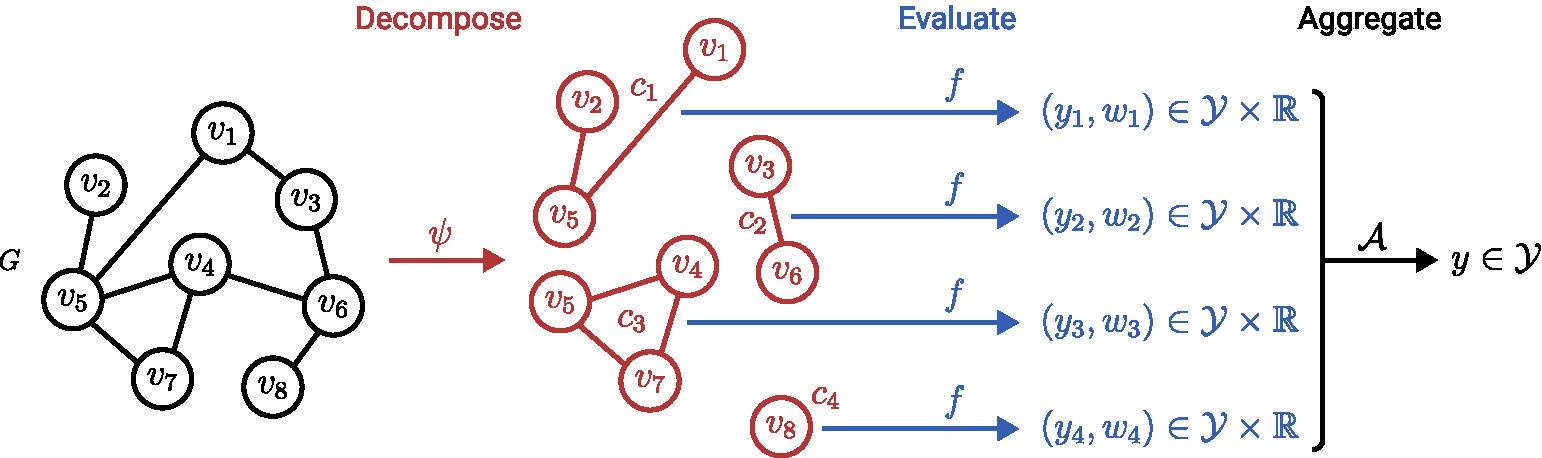
\includegraphics[width=\linewidth]{gfx/graph-lta/ltag-overview.pdf}
	\caption{
		Overview of the generalized \ac{lta} architecture for structured data.
	}\label{fig:ltag:ltag-overview}
\end{figure}
Based on the notion of decomposition, local evaluation and aggregation we can now define the concept of \textit{\ac{lta} formulations}.
\begin{defn}
	A model $h: \mathcal{G} \to \mathcal{Y}$ is in an \textit{\ac{lta} formulation} iff.\ it is expressed as
	\begin{align*}
		h(G) \coloneqq \mathcal{A}(\ldblbrace f(c_{G,i})\, |\, c_{G,i} \in \psi(G) \rdblbrace) \quad\text{with $\psi$, $f$ and $\mathcal{A}$ as defined above.}
	\end{align*}
\end{defn}
Note that every model $h: \mathcal{G} \to \mathcal{Y}$ has a trivial recursive \ac{lta} formulation by choosing $\psi(G) = \{ G \}$, $f(G) = (h(G), 1)$ and an arbitrary weighted aggregation function $\mathcal{A}$.
Those trivial \ac{lta} formulations do not split compositions into locally evaluated constituents and therefore intuitively do not fulfill the postulated localized explainability characteristic of \ac{lta}.
However since there is no commonly accepted formal criterion to decide whether a model's decisions are explainable~\cite{Lipton2018}, we do not attempt to strictly distinguish between \ac{lta} and non-\acs{lta} methods.
Instead the notion of \ac{lta} formulations should be seen as way to identify how ``\acs{lta}-like'' a model is:
\begin{itemize}
	\item \textbf{Negative extreme:}
		If a model $h$ only has trivial \ac{lta} formulations with the decomposition function $\psi(G) = \{ G \}$, it is not considered to be an \ac{lta} model.
	\item \textbf{Positive extreme:}
		If a model has an \ac{lta} formulation with a decomposition function that returns interpretable constituents, it is considered to be an \ac{lta} model.
		By definition this is true for the single-vertex constituents $\psi(G) \coloneqq {\{ G[v_{c_i}] \}}_{v_{c_i} \in \mathcal{V}_G}$ of \ac{lta} methods for unstructured data.
	\item \textbf{In-between cases:}
		An \ac{lta} method for structured data must produce models that lie somewhere in-between the two extremes.
\end{itemize}

The more ``\acs{lta}-like'' a given model is, the stronger its bias towards locally explainable predictions, which in turn reduces the potential expressive power of the model.
\citet{Gilpin2018} describe this trade-off between explainability and expressive power in more detail.
However, when considering problem domains in which the true composition scores $y_G$ are accurately described by an \acs{lta}-like generative process, a less expressive \ac{lta}-like model could generalize better than a more expressive non-\ac{lta} model.
This idea is captured by the so-called \textit{\ac{lta} assumption}.
\begin{defn}
	A problem domain $\mathcal{D}$ satisfies the \textit{\ac{lta} assumption} iff.\ there is an \ac{lta} method which produces models with an equal or lower out-of-sample error than the models produced by non-\acs{lta} methods for most training samples $\mathcal{D}_{\text{train}} \subseteq \mathcal{D}$.
\end{defn}
Due to the fuzziness of the class of \ac{lta} methods, the \ac{lta} assumption is naturally also a fuzzy concept.
Nonetheless evidence for its truthiness in a given domain $\mathcal{D}$ can be empirically obtained by comparing candidate \ac{lta} methods with the best known non-\ac{lta} method for $\mathcal{D}$, assuming that some cut-off condition for the required ``\ac{lta}-ness'' of an \ac{lta} method is agreed upon.

\section{\acs*{lta} Formulations of Existing \acs*{gcr} Methods}%
\label{sec:ltag:formulation}

Based on the general definition of \ac{lta} from the last section, we will now see to what extent the \ac{gcr} methods described in \cref{sec:related:gcr} can be interpreted as \ac{lta} instances.
First the relation between \acp{svm} on graph embeddings and \ac{lta} will be explored.
Then we will provide an \ac{lta} perspective on \acp{gcnn}.

\subsection{\acsp*{svm} on Graph Embeddings as \acs*{lta} Models}%
\label{sec:ltag:formulation:svm}

In \cref{sec:related:gcr:embed,sec:related:gcr:kernel} three different ways to map a given graph $G$ to a vector $\varphi(G) \in \mathbb{R}^d$ were described:
\begin{enumerate*}
	\item Fingerprint embeddings,
	\item skip-gram inspired embeddings and
	\item kernel embeddings
\end{enumerate*}.
One common way to solve the \ac{gcr} problem via those embedding vectors is to train an \ac{svm} on them.
We will now see that \acp{svm} can be interpreted as \ac{lta} models if they are trained on so-called \acp*{sce}.
\begin{defn}
	Given a a multiset $A = \ldblbrace \underbrace{a_1, \dots, a_1}_{\gamma_A(a_1)\text{ times}},\allowbreak \dots, \underbrace{a_n, \dots, a_n}_{\gamma_A(a_n)\text{ times}} \rdblbrace \subseteq D$, the so-called \textit{multiplicity function} $\gamma_A: D \to \mathbb{N}_0$ maps each element of the domain $D$ to its multiplicity in $A$ with $\gamma_A(x) = 0 \Leftrightarrow x \notin A$.
\end{defn}
\begin{defn}\label{defn:ltag:substruct-embedding}
	A graph embedding $\varphi: \mathcal{G} \to \mathbb{N}_0^{d}$ is called a \ac{sce} iff.\ %
	there are decomposition functions $\psi_{\varphi, i}: \mathcal{G} \to \mathcal{P}(\mathcal{G})$ and multiplicity functions $\gamma_{\varphi, i}: \mathcal{G} \to \mathbb{N}_0$ for all embedding components $i \in [d]$ s.t.\ %
	$\forall G \in \mathcal{G}, i \in [d]: \varphi(G)[i] = \sum_{c \in \psi_{\varphi, i}(G)} \gamma_{\varphi, i}(c)$ where $\gamma_{\varphi, i}$ is the multiplicity function of a multiset of the constituents $\psi_{\varphi, i}(G)$.
	We call $\psi_{\varphi, i}$ an \textit{underlying decomposition} of the $i$-th component of the embedding $\varphi$.
	Similarly the joint decomposition $\psi_{\varphi}(G) \coloneqq \bigcup_{i=1}^d \psi_{\varphi,i}(G)$ is an \textit{underlying decomposition} of $\varphi$.
\end{defn}
Intuitively \cref{defn:ltag:substruct-embedding} states that the value of each \ac{sce} component must be derived from the number of constituents produced by some decomposition function where each constituent might be counted multiple times.
Based on this requirement we now proof the main theorem which shows the relation between \acp{svm} and \ac{lta}.

\begin{thm}\label{thm:ltag:svm-ltag-formulation}
	A binary \ac{svm} graph classifier $h$ that applies a \ac{sce} $\varphi$ to its inputs has an \ac{lta} formulation that uses an underlying decomposition $\psi_{\varphi}$ of $\varphi$.
\end{thm}
\begin{proof}
	Let $h: \mathcal{G} \to {\{ -1, +1 \}}$ be a binary graph classifier expressed as $h = h_{\text{\acs*{svm}}} \circ \varphi$ where $\varphi: \mathcal{G} \to \mathbb{N}_0^{d}$ is an \ac{sce} and $h_{\text{\acs*{svm}}}: \mathbb{R}^{d} \to {\{ -1, +1 \}}$ a standard \ac{svm} classifier.
	Additionally, let $\psi_{\varphi}$ be some underlying decomposition of $\varphi$ with ${\{ \gamma_{\varphi, i} \}}_{i=1}^d$ being the corresponding multiplicity functions.

	Based on this decomposition we now bring the \ac{svm} graph classifier $h$ into an \ac{lta} formulation.
	If $h$ is trained on a dataset $\mathcal{D}_{\text{train}} = {\{ (G_1, y_1), \dots, (G_N, y_N) \}}$, via the kernel trick it can be expressed as
	\begin{align*}
		h(G) &= \sgn\left( \sum_{j = 1}^{N} \alpha_j y_j {\langle \varphi(G), \varphi(G_j) \rangle} + b \right)
		\quad\text{for some $\alpha \in \mathbb{R}_{\geq 0}^N$ and $b \in \mathbb{R}$} \\
		&= \sgn\left( {\sum_{i=1}^{d} {
				\varphi(G)[i]
				\underbrace{\left( \sum_{j = 1}^{N} \alpha_j y_j {\varphi(G_j)}[i] \right)}_{\beta_i}}
			} + b \right)
		 = \sgn\left( {\sum_{i=1}^{d} \varphi(G)[i] \beta_i} + b \right) \\
		&= \sgn\left( {\sum_{c_t \in \psi_{\varphi}(G)} \underbrace{\sum_{i = 1}^d \gamma_{\varphi, i}(c_t) \beta_i}_{z_t}} + b \right)
		 = \sgn\left( {\sum_{c_t \in \psi_{\varphi}(G)}} \underbrace{|z_t|}_{w_t} \underbrace{\sgn{z_t}}_{y_t} + {\underbrace{|b|}_{w_b} \underbrace{\sgn{b}}_{y_b}} \right) \\
		&= \wmaj\left( \ldblbrace (y_t, w_t)\, |\, c_t \in \psi_{\varphi}(G) \rdblbrace \cup \ldblbrace (y_b, w_b) \rdblbrace \right)
		\text{.}
	\end{align*}
	By choosing $f_h(c_t) \coloneqq (y_t, w_t)$ and $\mathcal{A}_h(S) = \wmaj(S \cup \ldblbrace (y_b, w_b) \rdblbrace)$, the \ac{svm} model therefore has an \ac{lta} formulation with the decomposition function $\psi_{\varphi}$.

	To complete the proof it now remains to show that $f_h$ and $\mathcal{A}_h$ are in fact a local evaluation function and a weighted aggregation function respectively.
	To see that $f_h$ perform local evaluation, note that $f_h(c_t) \coloneqq (\sgn z_t, {|z_t|})$ with $z_t \coloneqq \sum_{i=1}^{d} \gamma_{\varphi,i}(c_t) \beta_i$ only depends on the shared multiplicity functions $\gamma_{\varphi,i}$, the constants $\beta_i$ and the constituent $c_t$;
	apart from $c_t$ no other information from the input graph $G$ is required by $f_h$ which makes it a local evaluation function.
	To see why $\mathcal{A}_h$ satisfies \cref{defn:ltag:weighted-agg}, note that it inherits the idempotency property from $\wmaj$ because $\mathcal{A}_h$ ignores the bias ``pseudo-constituent'' $(y_b, w_b)$ for all threshold weights $\max w_t \geq \eta > w_b$, similarly the zero invariance of $\wmaj$ is also directly inherited.
	This concludes the proof.
\end{proof}

The central statement of \cref{thm:ltag:svm-ltag-formulation} is that \acs{svm} graph classifiers that use an \ac{sce} $\varphi$ implicitly perform an \acs{lta}-like weighted majority vote aggregation of constituent scores $y_t$.
Those constituent scores can in turn be expressed as a majority vote of the graph scores in the training dataset $\mathcal{D}_{\text{train}}$:
\begin{align}
	y_t \coloneqq \sgn z_t
	 &= \sgn\left( \sum_{j=1}^N \underbrace{\left( \alpha_j \smashoperator[l]{\sum_{c_k \in \psi_{\varphi}(G_j)}} \sum_{i=1}^d \gamma_{\varphi,i}(c_t) \gamma_{\varphi,i}(c_k) \right)}_{w_j} y_j \right) \\
	 &= \wmaj(\ldblbrace (y_j, w_j)\, |\, j \in [N] \rdblbrace) \nonumber
\end{align}
Note that, if the constituents of $G_j$ all come from different embedding components than those of $G$ ($\forall i \in [d]: {\psi_{\varphi, i}(G_j) \cap \psi_{\varphi, i}(G)} = \emptyset$), then $G_j$ has no influence on the score of $G$ ($w_j = 0$).

To see what \cref{thm:ltag:svm-ltag-formulation} implies in practice, we will now apply it to the graph embedding approaches described in \cref{sec:related:gcr:embed,sec:related:gcr:kernel}:
\begin{enumerate}[label=\textbf{\arabic*.}]
	\item \textbf{Fingerprint embeddings:}
		Here the $i$-th embedding component represent the number of occurrences of a substructure $S_i$, i.e.\ ${\varphi}_{\text{FP}}(G)[i] \coloneqq \mathit{count}_{S_i}(G)$ (see \cfullref{defn:related:wl-count-detect}).
		Such a fingerprint embedding naturally is an \ac{sce} with the decomposition functions $\psi_{\text{FP}, i}(G) \coloneqq \{ G[\set(s)]\, |\, s \in \mathcal{V}_G^{*} \land G[s] \equiv S_i \}$ and the multiplicity functions $\gamma_{\text{FP}, i}(c) \coloneqq \mathbbm{1}[c \simeq S_i]$ since those functions produce the subgraphs that are counted by ${\varphi}_{\text{FP}}(G)[i]$ with multiplicity $1$. % chktex 21

		Under the assumption that the substructure patterns $S_i$ are chosen s.t.\ the their instances $c \in \psi_{\text{FP}, i}(G)$ are nontrivial interpretable constituents, the underlying joint decomposition $\psi_{\text{FP}}(G) \coloneqq \bigcup_{i=1}^d \psi_{\text{FP}, i}(G)$ must also be nontrivial and interpretable.
		Thus, by \cref{thm:ltag:svm-ltag-formulation}, \acp{svm} trained on fingerprint embeddings are \ac{lta} models that produce locally explainable predictions.
		\badgebox[t_green]{LTA}
	\item \textbf{\texttt{graph2vec}:}
		The skip-gram inspired \texttt{graph2vec} embedding produces vectors $\varphi(G) \in \mathbb{R}^d$ whose individual components do not have a clear interpretation.
		\texttt{graph2vec} embeds graphs that have common 1-\acs{wl} colors closer to each other than graphs that do not share the same colors (see \cfullref{eq:related:graph2vec}).
		The resulting component values can be arbitrary reals, therefore this approach is not an \ac{sce} which in turn implies that it does not have an \ac{lta} formulation as in \cref{thm:ltag:svm-ltag-formulation}.
		\badgebox[t_red]{non-LTA}
	\item \textbf{\ac{wl} subtree kernel:}
		The individual components of the \ac{wl} subtree kernel's embedding $\varphi_{\text{ST}}$ represent the number of occurrences of a color $\kappa_i \in \mathcal{C}$, i.e.\ $\varphi_{\text{ST}}(G)[i, t] \coloneqq \mathit{dist}_{\chi_{G,1}^{(t)}}(\kappa_i)$ as defined in \cfullref[ on ]{eq:related:wl-subtree-kernel}\footnote{
			To avoid confusion $\kappa_i \in \mathcal{C}$ is used for colors and $c_j \in \mathcal{G}$ for constituents in this context.
		}.
		The occurrence of a color $\kappa_i$ at some vertex $v_j \in \mathcal{V}_G$ in the $t$-th refinement step (i.e.\ $\chi_{G,1}^{(t)}(v_j) = \kappa_i$) in turn implies that the \ac{bfs} tree $S_{j,t} \coloneqq \text{\acs*{bfs}}(G, v_j, t)$ of depth $t$ rooted at $v_j$ is isomorphic to some \ac{wl} color subtree $S_{\kappa_i}$ (i.e.\ $S_{j,t} \simeq S_{\kappa_i}$).
		This relation between \ac{wl} colors $\kappa_i$ and subtrees $S_{\kappa_i}$ was illustrated in \cfullref[ on ]{fig:related:wl-subtree}.

		To show that $\varphi_{\text{ST}}$ is an \ac{sce}, we have to define decomposition functions $\psi_{\varphi, i, t}$ and multiplicity functions $\gamma_{\varphi, i, t}$ s.t.\ $\varphi(G)[i, t] = \sum_{c \in \psi_{\varphi, i, t}(G)} \gamma_{\varphi, i, t}(c)$.
		Since $\varphi(G)[i, t]$ counts the occurrences $S_{j,t}$ of a subtree $S_{\kappa_i}$ in $G$, the \ac{sce} requirement would be trivially satisfied if each $S_{j,t}$ were a constituent with multiplicity $1$.
		This intuition is however not quite correct because the constituents of a graph $G$ must be induced subgraphs of $G$, not \ac{bfs} subtrees $S_{j, t}$ of $G$.
		\begin{figure}[t]
			\centering
			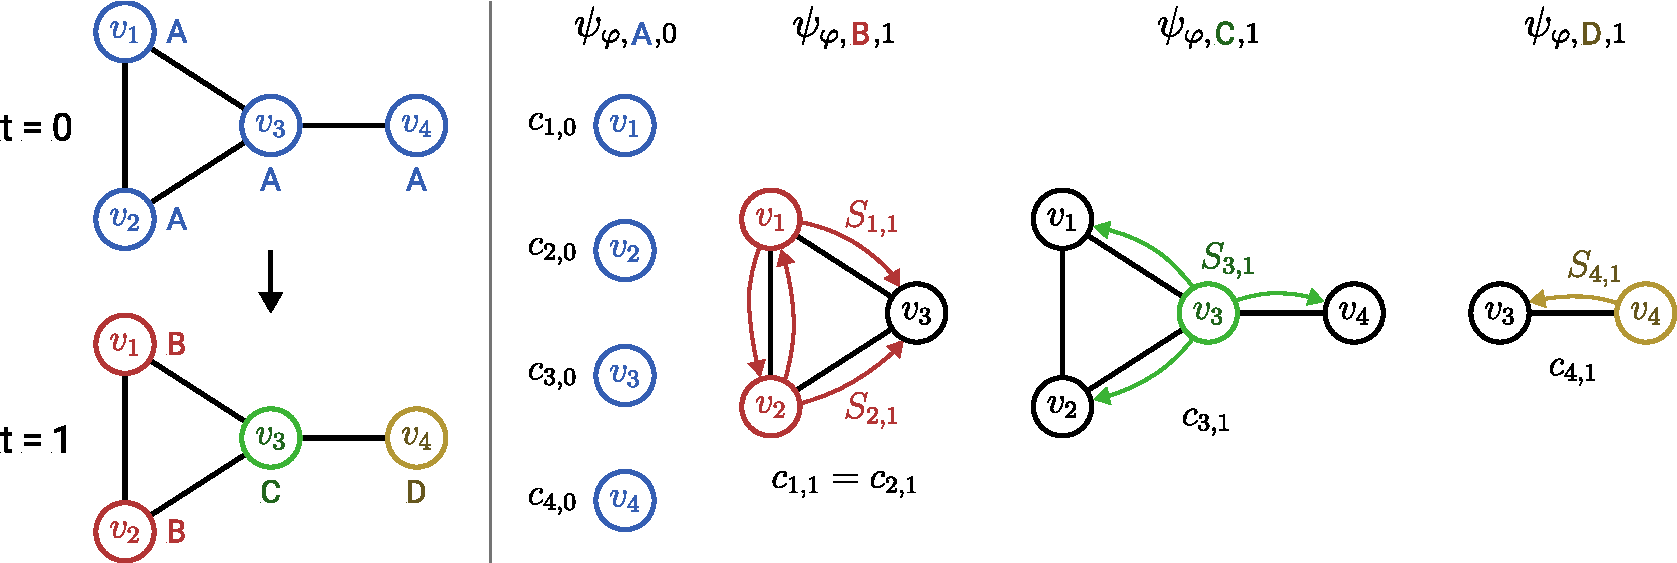
\includegraphics[width=\linewidth]{gfx/graph-lta/wl1-constituents.pdf}
			\caption[The constituents implied by the \ac{wl} subtree kernel embedding for an example graph.]{
				The constituents $c_{j,t}$ implied by the \ac{wl} subtree embedding vector $\varphi(G) = (\underbrace{\textcolor{t_blue}{4}, \textcolor{t_red}{0}, \textcolor{t_green}{0}, \textcolor{t_darkyellow}{0}}_{t = 0}, \underbrace{\textcolor{t_blue}{0}, \textcolor{t_red}{2}, \textcolor{t_green}{1}, \textcolor{t_darkyellow}{1}}_{t = 1})$. % chktex 25
				The subtrees $S_{j,t}$ that span each constituent $c_{j,t}$ are visualized by the colored arrows that originate from the colored root vertices.
				Because $S_{1,1}$ and $S_{2,1}$ span the same constituent $c = c_{1,1} = c_{2,1} = G[\{ v_1, v_2, v_3 \}]$, its multiplicity is $\gamma_{\varphi, \textcolor{t_red}{\texttt{B}}, 1}(c) = 2$; % chktex 25
				the multiplicity of all other constituents is $1$.
			}\label{fig:ltag:wl1-constituents}
		\end{figure}

		To fix the previous intuition we ``convert'' the subtrees $S_{j, t}$ into proper subgraph constituents via $c_{j,t} \coloneqq G[\mathcal{V}_{S_{j,t}}]$, i.e.\ the subgraphs that are spanned by the subtrees.
		The resulting decomposition functions are $\psi_{\varphi, i, t}(G) \coloneqq \{ c_{j,t}\, |\, {v_j \in \mathcal{V}_G}\,\land {S_{j,t} \simeq S_{\kappa_i}} \}$. % chktex 21
		As illustrated in \cref{fig:ltag:wl1-constituents}, the number of distinct constituents $c_{j,t}$ might be smaller than the number of \ac{bfs} subtrees $S_{j,t}$ because two distinct subtrees might span the same set of vertices.
		To fix this discrepancy between the subtree occurrence count (which equals $\varphi(G)[i, t]$) and the number of constituents, the multiplicities $\gamma_{\varphi, i, t}(c)$ of the constituents $c$ have to correspond to the number of \ac{bfs} subtrees they were spanned up by, i.e.\
		\begin{align*}
			\gamma_{\varphi, i, t}(c) &\coloneqq {|\{ S = \text{\acs*{bfs}}(c, v_{\text{root}}, t)\, |\, v_{\text{root}} \in \mathcal{V}_c \land S \simeq S_{\kappa_i} \land \mathit{complete}(S) \}|} \\
			\text{with }\mathit{complete}(S) &\Leftrightarrow \forall\ \text{leaf nodes $v_{\text{leaf}}$ of the tree $S$}: {|\Gamma_c(v_{\text{leaf}})|} = {|\Gamma_G(v_{\text{leaf}})|}
			\text{.}
		\end{align*}
		The purpose of the $\mathit{complete}(S)$ condition is to only count the \ac{bfs} subtrees of the constituent $c$ that are also \ac{bfs} subtrees of the complete graph $G$.
		To see why this is required, note that in \cref{fig:ltag:wl1-constituents} the $c_{1,1}$/$c_{2,1}$ constituent contains the color subtree $S_{\textcolor{t_red}{\texttt{B}}}$ three times (rooted at $v_1$, $v_2$ and $v_3$) even though $G$ only contains it twice (rooted at $v_1$ and $v_2$). % chktex 25
		Also note that, since $\gamma_{\varphi, i, t}(c)$ must only depend on a given constituent $c$ and not on the graph $G$ it was decomposed from, the degree information $|\Gamma_G(v_{\text{leaf}})|$ of the constituent vertices $v \in \mathcal{V}_c$ is assumed to be statically encoded in the labels $l_c[v]$ or feature vectors $x_c[v]$.

		Via the decomposition and multiplicity functions that were just described, $\varphi_{\text{ST}}$ is in fact an \ac{sce} with a nontrivial, subtree-based decomposition function.
		By \cref{thm:ltag:svm-ltag-formulation} \acp{svm} that use the \ac{wl} subtree kernel therefore have nontrivial \ac{lta} formulations, i.e.\ they can be considered to be ``\ac{lta}-like'' models.
		However, unlike fingerprint embeddings, the \ac{wl} subtree constituents are not manually chosen to be interpretable.
		This implies that the localized explainability characteristic of \ac{lta} is only partially satisfied since the \ac{svm} predictions are based on local constituent predictions that are not necessarily interpretable.
		\badgebox[t_green]{LTA-like}
	\item \textbf{\ac{wl} shortest path kernel:}
		\badgebox[t_red]{non-LTA}
	\item \textbf{$k$-LWL kernel:}
		\badgebox[t_green]{LTA-like}
	\item \textbf{$k$-GWL kernel:}
		\badgebox[t_red]{non-LTA}
\end{enumerate}

\subsection{\acsp*{gcnn} as \acs*{lta} Models}%
\label{sec:ltag:formulation:gcnn}

\section{A Novel \acs*{lta}-Inspired \acs*{gcnn} Architecture}%
\label{sec:ltag:wl2gnn}

%!TEX root = ../main.tex
% chktex-file 46
\chapter{Evaluation}%
\label{sec:eval}

In \cref{sec:ltag} the relation between \ac{lta} and existing \ac{gcr} approaches was formally analyzed.
There we saw that the \ac{lta} formulations of existing approaches mostly use static decomposition functions, e.g.\ \ac{bfs} subtree decompositions.
Motivated by the idea of dynamically learning decompositions via edge filters, we then proposed the novel 2-\acs{wl}-\acs{gnn} in \cref{sec:ltd}.
The ideas presented in both chapters will now be empirically evaluated.
To do so we differentiate between two mostly independent evaluation aspects:
\begin{enumerate}[label={\textbf{\arabic*.}}]
	\item \textbf{Evaluation of 2-\acs{wl}-\acsp{gnn}:}
		Even though it was motivated by \ac{lta}, a 2-\acs{wl}-\acs{gnn} is not generally more ``\acs{lta}-like'' than other approaches.
		Nonetheless, due to the theoretical advantages described in \cref{sec:ltd:wl2gnn:properties}, it is an interesting approach independently from its potential applications in \ac{lta} (see \cref{sec:ltd:edge-filter}).
		Thus the first aspect of our evaluation is to compare 2-\acs{wl}-\acsp{gnn} with the other previously described \ac{gcr} methods in a general non-\acs{lta} fashion, i.e.\ with an added \ac{mlp} after the pooling layer since this is how \acp{gnn} are typically evaluated in other works.
	\item \textbf{Evaluation of the \ac{lta} assumption:}
		We previously described that a given domain problem satisfies the \ac{lta} assumption if its solutions can be described by an \ac{lta} formulation (see \cfullref{defn:ltag:lta-assumption}).
		The inherent bias of an \acs{lta}-like model towards such \ac{lta} formulations could potentially increase its generalization performance compared to more general non-\acs{lta} models.
		Therefore the second aspect of our evaluation is to compare the performance of the previously described \acs{lta}-like methods with that of non-\acs{lta} approaches on datasets from multiple problem domains.
\end{enumerate}
This chapter will tackle those two aspects in four steps:
\begin{enumerate*}[label={\circled{\small\arabic*}}]
	\item We begin by describing the experimental setup used to obtain the evaluation results in \cref{sec:eval:setup}.
	\item We then present results on synthetically generated data in \cref{sec:eval:synthetic}.
	 	There we will illustrate the higher expressive power of 2-\acs{wl}-\acsp{gnn} when compared to other \ac{gcr} approaches, which confirms the theoretical results from \cref{sec:ltd:wl2gnn:properties}.
	\item Then evaluation results on real-world datasets are described in \cref{sec:eval:real}.
		There we will see how 2-\acs{wl}-\acsp{gnn} compare to other \acp{gnn} in practice as well as how \acs{lta}-like models compare to non-\acs{lta} models.
	\item Finally, \cref{sec:eval:lta} looks at the synthetic and real-world results from an \ac{lta} perspective.
		There we will see how the predictive performance of an \acs{lta}-like model relates to the size and locality of its constituents.
\end{enumerate*}

\section{Experimental Setup}%
\label{sec:eval:setup}

In our experimental evaluation we focus on two types of learners:
\acp{svm} using graph kernels and \acp{gcnn}.
We evaluate those learners by comparing their test accuracies on multiple binary classification problems.
To obtain those accuracies we follow the graph classification benchmarking framework recently proposed by \citet{Errica2020}.
Their benchmarking framework is motivated by the observation that most recent publications in the field of \acp{gnn} do not provide reproducible results.
To tackle this issue they evaluated multiple state-of-the-art methods using a unified model selection procedure:\\
{\setlength{\intextsep}{0pt}%
\begin{minipage}[t]{0.55\linewidth-1em}
	\begin{algorithm}[H]
		\caption{$k$-fold Model Assessment}\label{algo:eval:assessment}
		\begin{algorithmic}[1]
			\State{\textbf{Input:} Dataset $\mathcal{D}$, configurations $\Theta$}
			\State{Split $\mathcal{D}$ into $k$ folds $F_1, \dots, F_{k}$}
			\For{$i \leftarrow 1, \dots, k$}
				\State{$\mathcal{D}_{\mathrm{train/val}}, \mathcal{D}_{\mathrm{test}} \leftarrow \left( \bigcup_{j \neq i} F_{j} \right), F_i$}
				\State{Split $\mathcal{D}_{\mathrm{train/val}}$ into $\mathcal{D}_{\mathrm{train}}, \mathcal{D}_{\mathrm{val}}$}
				\State{$\theta_{\mathrm{best}} \leftarrow \Call{Select}{\mathcal{D}_{\mathrm{train}}, \mathcal{D}_{\mathrm{val}}, \Theta}$}
				\For{$r \leftarrow 1, \dots, R$}
					\State{$h_{i,r} \leftarrow \Call{Train}{\mathcal{D}_{\mathrm{train}}, \theta_{\mathrm{best}}}$}
					\State{$\mathit{acc}_{i,r} \leftarrow \Call{Eval}{h_{i,r}, \mathcal{D}_{\mathrm{test}}}$}
				\EndFor{}
				\State{$\mathit{acc}_{i} \leftarrow \mean_{r \in [R]}{\mathit{acc}_{i,r}}$}
			\EndFor{}
			\State{\Return{$\mean_{i \in [k]} \mathit{acc}_i, \mathrm{stddev}_{i \in [k]}\, \mathit{acc}_i$}}
		\end{algorithmic}
	\end{algorithm}
\end{minipage}\hspace*{1em}%
\begin{minipage}[t]{0.45\linewidth}
	\begin{algorithm}[H]
		\caption{Model Selection}\label{algo:eval:selection}
		\begin{algorithmic}[1]
			\Function{Select}{$\mathcal{D}_{\mathrm{train}}, \mathcal{D}_{\mathrm{val}}, \Theta$}
			\ForAll{$\theta \in \Theta$}
				\State{$h_{\theta} \leftarrow \Call{Train}{\mathcal{D}_{\mathrm{train}}, \theta}$}
				\State{$\mathit{acc}_{\theta} \leftarrow \Call{Eval}{h_{\theta}, \mathcal{D}_{\mathrm{val}}}$}
			\EndFor{}
			\State{$\theta_{\mathrm{best}} \leftarrow \arg\max_{\theta \in \Theta}{\mathit{acc}_{\theta}}$}
			\State{\Return{$\theta_{\mathrm{best}}$}}
			\EndFunction{}
		\end{algorithmic}
	\end{algorithm}
\end{minipage}}

We base our evaluations on this assessment strategy with $k = 10$ folds and $r = 3$ repeats per fold to smooth out differences caused by random weight initializations.
For each dataset, the same folds are used across the evaluated models; class proportions are preserved within each fold by using stratified splits.
To keep the total runtime of the experiments feasible, a single 90\%/10\% holdout split into training and validation data is used instead of cross-validation.
To train models that require gradient-based optimization, we use the well-known Adam optimizer~\cite{Kingma2015} and the standard binary crossentropy loss.
In all experiments, training is performed with an early stopping condition which cancels the optimization if there is no improvement to the validation loss for more than $p$ epochs.
The patience period $p$ is part of the hyperparameter configurations $\theta \in \Theta$.

Using this assessment strategy, we evaluate \acp{svm} with the following graph kernels:
\begin{enumerate}[label={\textbf{\arabic*.}},itemsep=2pt,parsep=2pt]
	\item \textbf{\ac{wl} subtree kernel (\acs{wl}\textsubscript{ST})} with the iteration counts $T \in \{ 1,2,3,4,5 \}$, to evaluate the influence of the depth of \ac{bfs} subtrees which span \ac{lta} constituents.
	\item \textbf{\ac{wl} shortest path kernel (\acs{wl}\textsubscript{SP})} with the iteration count $T = 3$.
	\item \textbf{2-LWL kernel} with the iteration count $T = 3$.
	\item \textbf{2-GWL kernel} with the iteration count $T = 3$.
\end{enumerate}
The gram matrices of the \acs{wl}\textsubscript{ST} and \acs{wl}\textsubscript{SP} kernels are computed via the \citetitle{GK} library~\cite{Siglidis2018}\cite{GK}.
For the gram matrices of the two dimensional \ac{wl} kernels we use a modified version\footnote{\url{https://github.com/Cortys/glocalwl}} of the reference implementation provided by \citet{Morris2017}.
To train \acp{svm} with those kernels, \citetitle{SKL}~\cite{Pedregosa2011}\cite{SKL} is used.
For the evaluation of \acp{gcnn} we selected the following methods:
\begin{enumerate}[label={\textbf{\arabic*.}},itemsep=2pt,parsep=2pt]
	\item \textbf{Structure unaware baseline:}
		\citet{Errica2020} describe a simple model which applies a standard \ac{mlp} to each individual vertex feature vector, then sums up the resulting feature vectors and applies another \ac{mlp} to the vector sum.
		This approach does not use any structural information and therefore serves as a baseline to detect whether a \ac{gnn} is able to exploit graph structure.
	\item \textbf{\ac{gin}} is evaluated as described by \citet{Xu2018}, i.e.\ with a sum pooling layer and an appended \ac{mlp} to produce the final prediction.
	\item \textbf{2-\acs{gnn}} is evaluated with both a static $\mean$ pooling layer and with \ac{sampool} (see \cfullref{defn:ltag:sam-pool}).
		After the pooling layer, an \ac{mlp} is used to produce the final prediction.
	\item \textbf{2-\acs{wl}-\ac{gnn}} \textit{(our method)} is also evaluated with $\mean$ pooling and \ac{sampool}, just like 2-\ac{gnn}.
		To test the \ac{lta} assumption, we evaluate 2-\acs{wl}-\acs{gnn} in an \acs{lta}-like configuration and in the standard non-\acs{lta} configuration.
		The \acs{lta}-like configuration uses a stack of 2-\acs{wl} convolutions that produce a local prediction $y_{ij} \in [0, 1]$ for each edge $e_{ij}$ instead of a local feature vector $z_{ij} \in \mathbb{R}^{d^{(T)}}$ and it does not have an \ac{mlp} after the pooling/aggregation layer.
\end{enumerate}
The baseline and \ac{gin} results are obtained using the PyTorch-based implementation provided by \citet{Errica2020}.
For both 2-\acs{gnn} and 2-\acs{wl}-\ac{gnn}, a custom TensorFlow-based implementation is used.
The code for all conducted experiments as well as the used dataset splits are available GitHub\footnote{\url{https://github.com/Cortys/master-thesis}}.
The evaluated hyperparameter configurations $\Theta$ are described in \cref{sec:appendix:config-grid}.

\section{Evaluation on Synthetic Data}%
\label{sec:eval:synthetic}

We begin with an evaluation of graph kernels and \acp{gnn} on a synthetic binary classification dataset which demonstrates the potential advantages of a higher dimensional \ac{wl} method such as the proposed 2-\acs{wl}-\acs{gnn}.
To determine the classes of the graphs in this dataset, a learner has to solve the so-called \textit{unicolored triangle detection} problem:
Given a graph $G$ with vertices that are colored as either $l_G[v] = \colorlabel{t_blue}{A}$ or as $l_G[v] = \colorlabel{t_red}{B}$, the learner has to find the unique triangle $(v_i, v_j, v_k)$ in $G$ for which $l_G[v_i] = l_G[v_j] = l_G[v_k]$. % chktex 25
The class of $G$ is then determined by the color of the vertices $(v_i, v_j, v_k)$.

Based on this problem, we generated a synthetic triangle detection dataset.
It contains randomly generated graphs with varying vertex counts and vertex color proportions (see \cref{sec:appendix:ds-stats} for a more detailed description).
We use this dataset to evaluate whether a learner is able to ignore varying amounts of noisy random structure and focus on relevant local substructures, in this case unicolored triangles.
For the evaluation of 2-\acs{wl}-\acsp{gnn}, the neighborhood radius $r = 2$ is used.
\begin{table}[t]
	\caption{Mean accuracies and standard deviations on the triangle detection dataset.}\label{tbl:eval:synthetic}
	\centering
	\csvreader[
		tabular={clrrr},
		separator=semicolon,
		table head={%
			& \multicolumn{2}{l}{Model (Iterations/Pooling)} & \multicolumn{1}{c}{Train} & \multicolumn{1}{c}{Test} \\\toprule%
		},
		table foot=\bottomrule,
		late after line=\ifthenelse{\equal{\id}{9}}{\\\midrule}{\\},
		head to column names,
		filter=\equal{\isDefault}{1}\or\equal{\id}{4}
	]{data/results.csv}{}{%
		\ifthenelse{\equal{\id}{0}}{\multirow{6}{*}[0em]{\rotatebox[origin=c]{90}{\small\textsc{Kernel}}}}{}%
		\ifthenelse{\equal{\id}{9}}{\multirow{8}{*}[0em]{\rotatebox[origin=c]{90}{\small\textsc{\ac{gnn}}}}}{} &%
		\textbf{\ifthenelse{\equal{\isLta}{1}}{\textcolor{t_darkgreen}{\model*}}{\model\ifthenelse{\equal{\model}{2-WL-GNN}}{\phantom{*}}{}}} ($\params$) & \ifthenelse{\equal{\isLta}{1}}{\badgeboxinline[t_green]{\scriptsize \acs*{lta}-like}}{} &%
		\evalres[\and\not\equal{\id}{8}]{\triangleBestTrain}{\triangleTrainMean}{\triangleTrainStd} & \evalres{\triangleBestTest}{\triangleTestMean}{\triangleTestStd}%
	}
\end{table}
\begin{figure}[t]
	\centering
	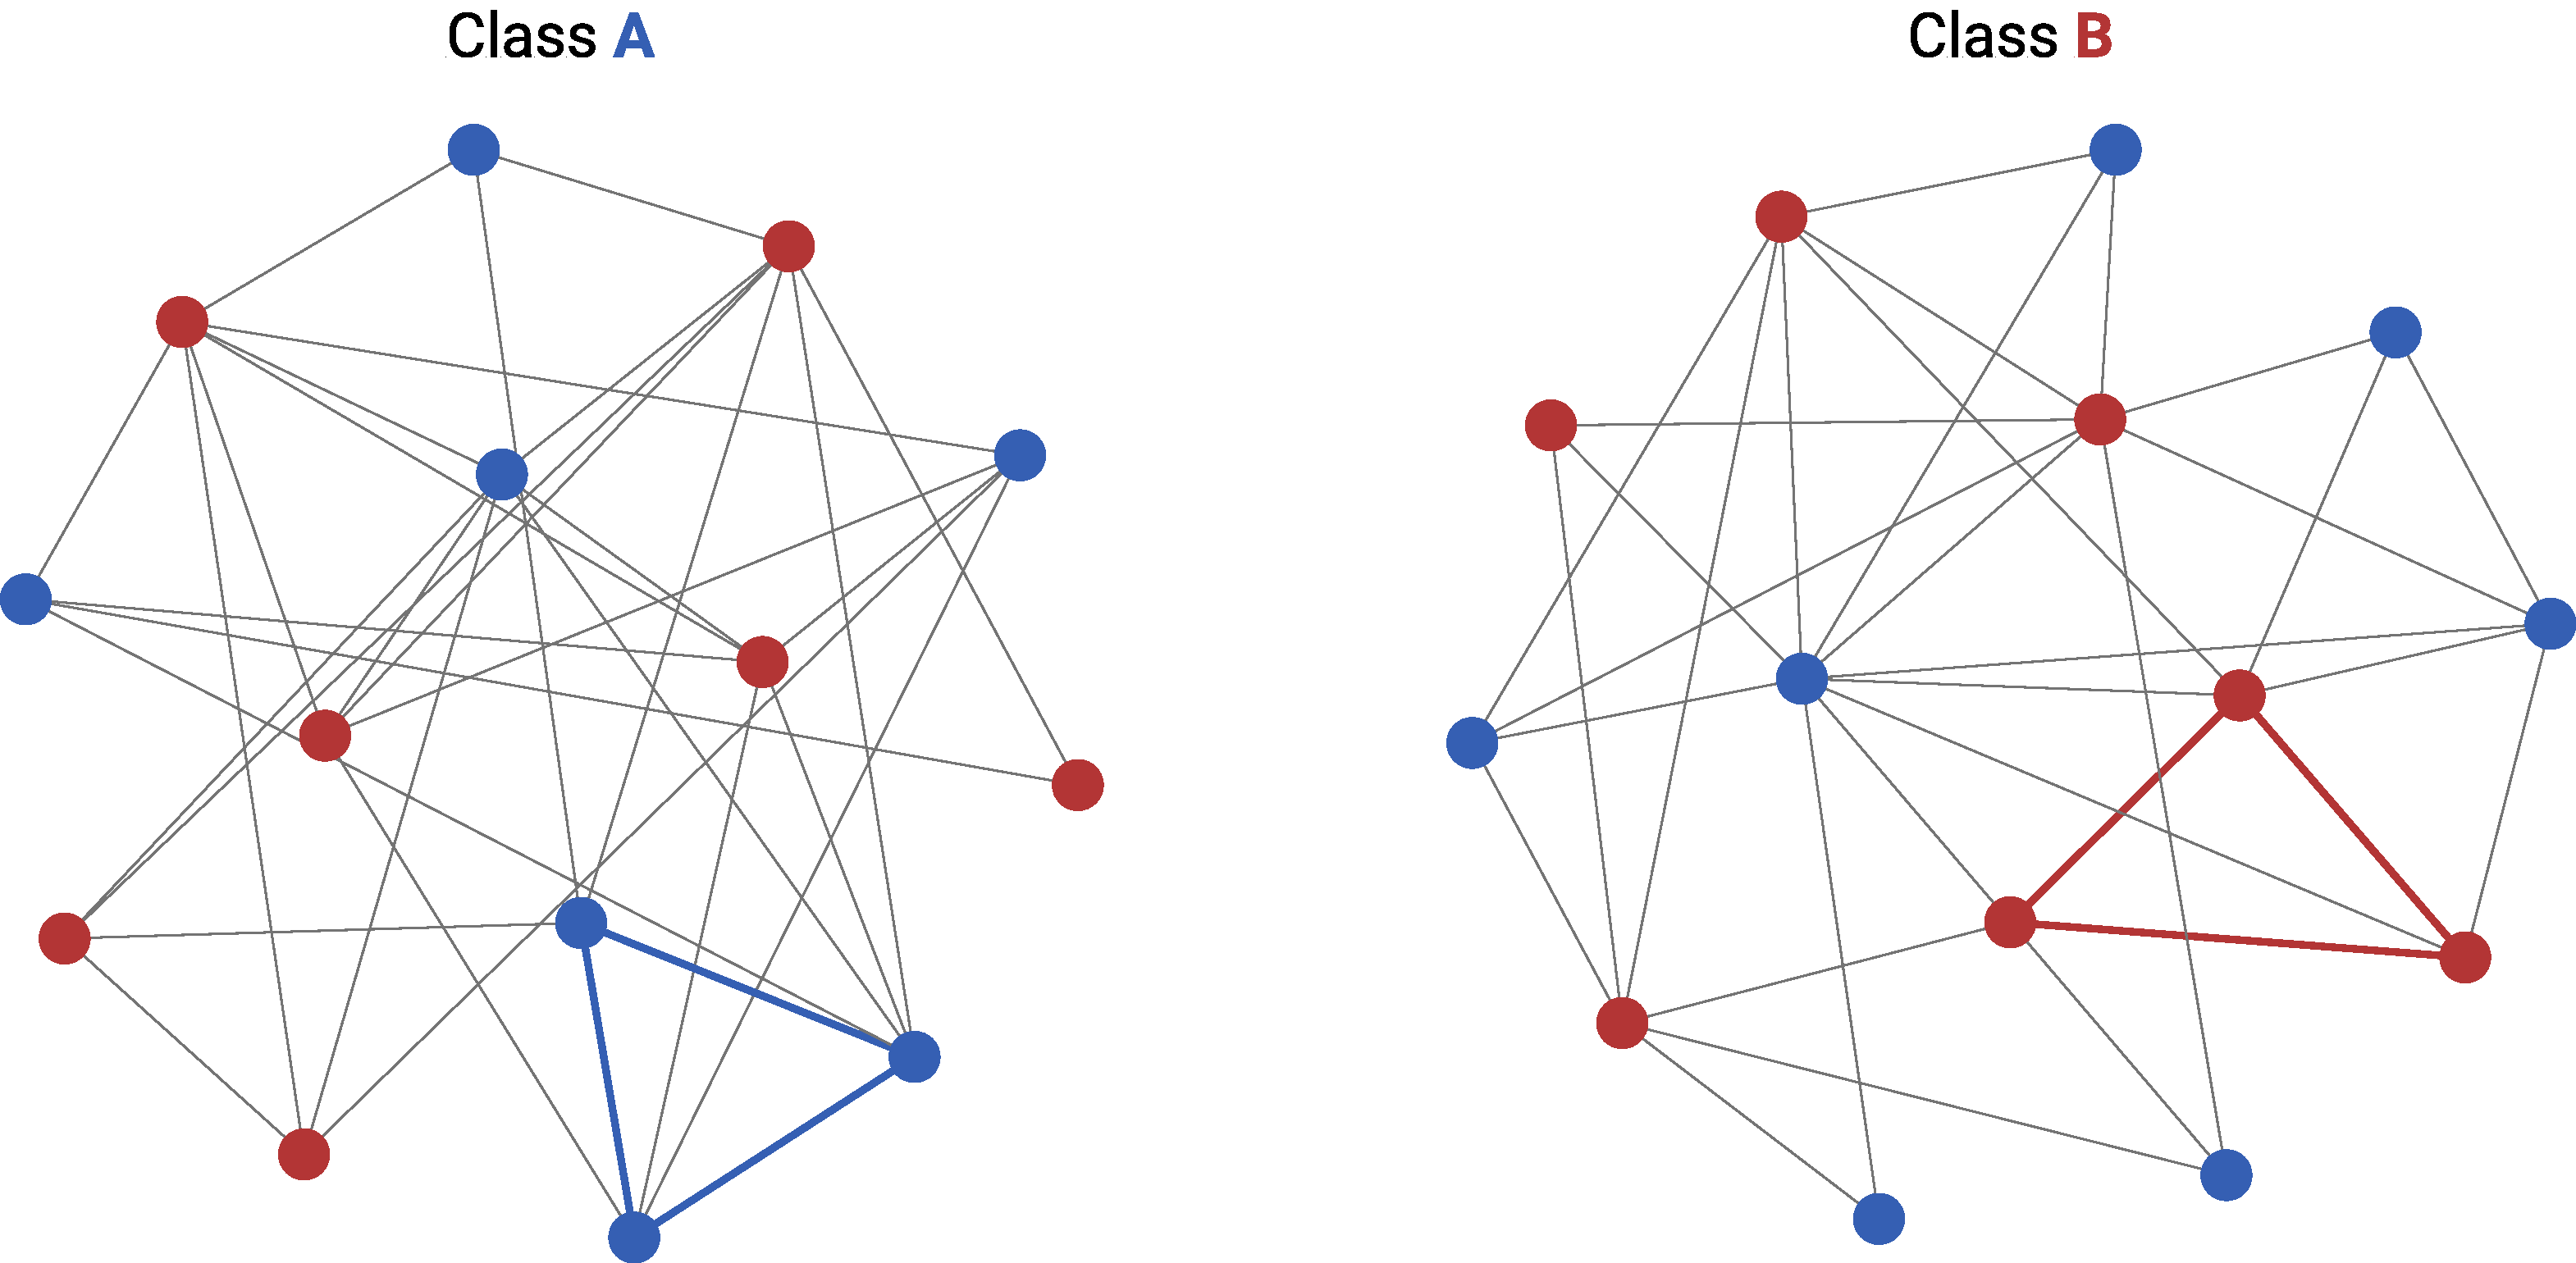
\includegraphics[width=0.7\linewidth]{gfx/evaluation/triangle-problem.pdf}
	\caption[Two example graphs from the triangle detection dataset.]{
		Two examples from the triangle detection dataset.
		The unique unicolored triangle, which has to be detected by the learners, is highlighted in both graphs.
	}\label{fig:evaluation:triangle-problem}
\end{figure}

Looking at the results in \cref{tbl:eval:synthetic}, it can be seen that the structure unaware baseline method is completely unable to detect triangles, as expected.
The structure aware learners on the other hand all perform better than random guessing and are in fact mostly able to fit the training data perfectly.
This shows that all generated graphs are 1-\acs{wl} distinguishable; the \ac{wl} subtree kernel \ac{svm}, for example, can simply ``memorize'' the training graphs via their unique 1-\acs{wl} color distribution after $T = 5$ refinement steps.

However, the ability to distinguish training graphs is not sufficient to also classify previously unseen graphs correctly.
Since 1-\acs{wl} cannot detect triangles, all 1-\acs{wl} bounded approaches (\acs{wl}\textsubscript{ST}, \acs{wl}\textsubscript{SP}, Baseline, \acs{gin}) are therefore unable to generalize, as can be seen in their test accuracies.
The fact that they perform better than random guessing can be explained by the following proxy indicator:
The presence of an \colorlabel{t_blue}{A}-colored triangle in a graph $G$ implies that there is a local region with a slightly higher density of \colorlabel{t_blue}{A}-colored vertices than in a \colorlabel{t_red}{B}-colored graph $H$ with the same vertex color proportions.
This local color density difference is already detectable in the depth-1 \acs{bfs} subtrees used by 1-\acs{wl} after a single refinement step; this explains why \acs{wl}\textsubscript{ST} performs similarly for $T = 1$ and $T = 5$.

Let us now take a look at the 2-\acs{wl} inspired kernels: 2-LWL and 2-GWL.\@
Interestingly, both kernels do not appear to generalize better the 1-\acs{wl} bounded methods;
we explain this by the fairly small size of the triangle detection dataset (228 graphs).
Even though both kernels embed graphs into a space with dimensions that indicate the presence of a unicolored triangle (see \cfullref{prop:related:wl2-cycle-count}), there are so many of those triangle-indicating embedding dimensions that the indicating dimensions found in a given training split might not overlap with those in the test split.

Looking at the 2-\acs{wl} inspired \acp{gnn} (2-\acs{gnn}, 2-\acs{wl}-\acs{gnn}), we find that the proposed 2-\acs{wl}-\acs{gnn} significantly outperforms all other evaluated methods, which confirms our theoretical results from \cref{sec:ltd:wl2gnn:properties}.
We evaluated 2-\acs{wl}-\acsp{gnn} in an \acs{lta}-like configuration without a final \ac{mlp} and in a non-\acs{lta} configuration with an \ac{mlp} after the pooling layer.
Comparing both configurations, we see that the \acs{lta}-variant has a worse generalization performance despite the fact that the triangle detection problem fits well into the \ac{lta} framework:
\begin{enumerate*}[label={\circled{\small\arabic*}}]
	\item Decomposition corresponds to finding a single unicolored triangle constituent,
	\item local evaluation then corresponds to checking the color of the triangle constituent and
	\item aggregation is trivial since there is only one constituent.
\end{enumerate*}

However, as we saw in the \ac{lta} formulation of \acp{gcnn} (see \cfullref{thm:ltag:gcnn-ltag-formulation}), a 2-\acs{wl}-\acs{gnn} does not actually learn to decompose a graph into unicolored triangle constituents but uses subtree constituents instead.
Further investigations are required to determine to which extent the worse performance of the \acs{lta}-like configuration is caused by this static decomposition strategy and whether a more dynamic solution to the \acf{ltd} problem could improve the performance (e.g.\ via the edge filtering idea described in \cref{sec:ltd:edge-filter}).

Finally, if we look at the two evaluated pooling layers, static $\mean$ pooling and \ac{sampool}, we see that the attention mechanism of the latter tends to improve the generalization performance of both 2-\acsp{gnn} and 2-\acs{wl}-\acsp{gnn}.
This indicates that \ac{sampool} is successful at filtering out the randomly generated noisy parts of a given graph and putting most attention to the relevant unicolored triangle.

\section{Evaluation on Real-World Data}%
\label{sec:eval:real}

\begin{table}[ht]
	\caption[Mean test accuracies and standard deviations on real-world data.]{
		Mean test accuracies and standard deviations on real-world data.
		\hfill\textcolor{t_darkgreen}{*}\,\badgeboxinline[t_green]{\scriptsize\acs*{lta}-like}
	}\label{tbl:eval:real}
	\centering
	\csvreader[
		tabular={lrrrrr},
		separator=semicolon,
		table head={%
			& %
			\multicolumn{1}{c}{\hyperref[tbl:appendix:diff-nci]{\textbf{NCI1}}} &%
			\multicolumn{1}{c}{\hyperref[tbl:appendix:diff-proteins]{\textbf{PROTEINS}}} &%
			\multicolumn{1}{c}{\hyperref[tbl:appendix:diff-dd]{\textbf{D\&D}}} &%
			\multicolumn{1}{c}{\hyperref[tbl:appendix:diff-reddit]{\textbf{REDDIT}}} &%
			\multicolumn{1}{c}{\hyperref[tbl:appendix:diff-imdb]{\textbf{IMDB}}}%
			\\\toprule%
		},
		table foot=\bottomrule,
		late after line=\ifthenelse{\equal{\id}{9}}{\\\midrule}{\\},
		head to column names,
		filter={\equal{\isDefault}{1}}
	]{data/results.csv}{}{%
		% \ifthenelse{\equal{\id}{0}}{\multirow{5}{*}[0em]{\rotatebox[origin=c]{90}{\small\textsc{Kernel}}}}{}%
		% \ifthenelse{\equal{\id}{9}}{\multirow{8}{*}[0em]{\rotatebox[origin=c]{90}{\small\textsc{\ac{gnn}}}}}{} &%
		\textbf{\ifthenelse{\equal{\isLta}{1}}{\textcolor{t_darkgreen}{\model*}}{\model\ifthenelse{\equal{\model}{2-WL-GNN}}{\phantom{*}}{}}} {\footnotesize($\params$)} &%
		{\small\evalres{\nciBestTest}{\nciTestMean}{\nciTestStd}}&%
		{\small\evalres{\proteinsBestTest}{\proteinsTestMean}{\proteinsTestStd}}&%
		{\small\evalres{\ddBestTest}{\ddTestMean}{\ddTestStd}}&%
		{\small\evalres{\redditBestTest}{\redditTestMean}{\redditTestStd}}&%
		{\small\evalres{\imdbBestTest}{\imdbTestMean}{\imdbTestStd}}%
	}
\end{table}
Since the synthetic triangle detection problem was designed specifically to highlight the advantages of a higher dimensional \ac{wl} method such as 2-\ac{wl}-\acsp{gnn}, we now evaluate the approaches more fairly on five common graph classification benchmark datasets from two different real-world domains:
\begin{enumerate}[label={\textbf{\arabic*.}}]
	\item \textbf{Bioinformatics:}
		The NCI1~\cite{Shervashidze2011}, PROTEINS~\cite{Borgwardt2005a} and D\&D~\cite{Dobson2003} datasets all contain molecular graphs.
		For NCI1 the goal is to predict whether a molecule is effective against certain types of cancer.
		For PROTEINS and D\&D, a learner has to determine whether a given protein molecule is an enzyme.
	\item \textbf{Social networks:}
		The REDDIT and IMDB datasets~\cite{Yanardag2015} contain graphs representing the relations between users in online discussions and movie actors respectively.
		For REDDIT, the type of a community has to be predicted based on a discussion thread; for IMDB, the goal is to determine movie genres.
\end{enumerate}
A more detailed description of the evaluated datasets can be found in \cref{sec:appendix:ds-stats}.
\Cref{tbl:eval:real} shows our evaluation results\footnote{
	Note that, for the NCI1, PROTEINS and D\&D datasets we used different training/test splits than those originally used by \citet{Errica2020}.
	The reason for this is that the original splits were only published after our evaluations of those datasets had already been completed.
	For REDDIT and IMDB however, we used the same splits.
	Also note that some values are missing because of \acf{oom} errors;
	the resource use for all evaluations was limited to \SI{64}{\giga\byte} main memory and \SI{11}{\giga\byte} GPU memory.
	On average, each \ac{gnn} assessment (as in \cref{algo:eval:assessment}) took about three days on an AMD 1800X 16-thread CPU and an Nvidia 1080~Ti GPU.% chktex 29
}.
For the evaluation of 2-\acs{wl}-\acsp{gnn}, different neighborhood radii were used for each dataset.
In the order of the columns in the table above, the results were obtained with the radii $r = 8$, $5$, $2$, $1$ and $4$ respectively.

If we compare the real-world results with those for the synthetic triangle detection dataset, we do no longer observe the clear advantage of 2-\acs{wl}-\acsp{gnn} over the other approaches.
This indicates that the theoretical advantages of 2-\acs{wl} over 1-\acs{wl} are not necessarily relevant for the five evaluated problems.
Nonetheless, the test performance of 2-\acs{wl}-\acsp{gnn} is generally comparable to that of the other state-of-the-art learners with the exception of NCI1,
where by comparable we mean that the performance of the evaluated 2-\acs{wl}-\acs{gnn} models is within the $2\sigma$ confidence interval of the best evaluated model even when compared fold-by-fold (see \cref{sec:appendix:fold-diffs}).

If we look at the enzyme detection problem (PROTEINS and D\&D), we observe that all evaluated approaches appear to be unable to leverage structural information for a significant improvement over the baseline learner (see \cref{tbl:appendix:diff-proteins,{tbl:appendix:diff-dd}}).
In the social network datasets (REDDIT and IMDB) on the other hand, the structure aware methods clearly outperform the baseline (see \cref{tbl:appendix:diff-reddit,tbl:appendix:diff-imdb}).
This confirms the very similar results of \citet{Errica2020}.

Lastly, note that the \acs{lta}-like 2-\acs{wl}-\acs{gnn} configurations either perform significantly worse or roughly similar to their non-\acs{lta} counterparts.
This mirrors our result on the synthetic triangle detection dataset.
Regarding the \acs{lta} assumption (see \cfullref{defn:ltag:lta-assumption}), this is evidence that the decomposition function $\psi$ of 2-\acs{wl}-\acsp{gnn} (see \cfullref{thm:ltag:gcnn-ltag-formulation}) does not produce constituents $c_i \in \psi(G)$ whose local evaluations $f(c_i) \in \mathcal{Y}$ are as indicative of the graph $G$'s class $y \in \mathcal{Y}$ as an arbitrary feature vector $z_i \in \mathbb{R}^{d^{(T)}}$.
This does however not imply that the evaluated real-world problem domains are generally incompatible with the \ac{lta} assumption.
When considering the results of the \ac{lta}-like \acs{wl}\textsubscript{ST} model, we find that it is mostly comparable with the alternative non-\acs{lta} approaches and, in the case of NCI1, even significantly better.
This shows that local constituent evaluations are in principle suitable for graph classification tasks if the right decomposition, evaluation and aggregation functions are chosen.

\section{Evaluation of \acs*{lta} Constituent Locality}%
\label{sec:eval:lta}

To conclude our evaluation, we now look at the influence of constituent sizes on the test accuracy of \acs{lta}-like models, such as \acs{wl}\textsubscript{ST} and 2-\acs{wl}-\acsp{gnn}.
As described in \cref{sec:ltag:formulation:svm,sec:ltag:formulation:gcnn:conv}, the constituents in the \ac{lta} formulations of both of these models are spanned by \ac{bfs} subtrees of some depth $T$.
Thus, for large $T$, decompositions consist of just the connected components of a graph, i.e.\ they are only partially \acs{lta}-like.

We now analyze for which degree of constituent locality \acs{wl}\textsubscript{ST} and 2-\acs{wl}-\acsp{gnn} perform best, by evaluating them using varying tree depths $T$.
For \acs{wl}\textsubscript{ST} we can set $T$ directly via the number of refinement steps.
\Cref{fig:eval:wlst-depths} shows the the accuracies of \acs{wl}\textsubscript{ST} for $T \in \{ 1, \dots, 5 \}$.
On all evaluated datasets, the test accuracy tends to be optimal for some $T \in \{ 1, 2, 3 \}$.%
\newcommand{\wlstDepthPlot}[4][ymin=70, ymax=100, try min ticks=6]{%
\begin{tikzpicture}
	\begin{axis}[
		width=0.35\linewidth,
		height=0.3\linewidth,
		xmin=0.7, xmax=5.3,
		#1,
		label style={font=\tiny},
		tick label style={font=\tiny},
		ymajorgrids,
		ytick style={draw=none},
		ylabel shift=-6pt,
		xlabel shift=-5pt,
		axis line style={gray},
		mark size={1.5pt},
		title={\small #3},
		title style={yshift=-0.5em}
	]
		\begin{scope}[gray]
			\draw[gray, dashed] ({axis cs:#4,0}|-{rel axis cs:0,1}) -- ({axis cs:#4,0}|-{rel axis cs:0,0});
		\end{scope}
		\addplot [color=t_blue, only marks, mark=*]
		plot[error bars/.cd, y dir=both, y explicit]
		table [x=T, y=#2TrainMean, y error=#2TrainStd, col sep=semicolon] {data/wlst_depths.csv};
		\label{pgfplots:eval:wlst-depth:#2-train}
		\addplot [color=t_red, only marks, mark=square*]
		plot[error bars/.cd, y dir=both, y explicit]
		table [x=T, y=#2TestMean, y error=#2TestStd, col sep=semicolon] {data/wlst_depths.csv};
		\label{pgfplots:eval:wlst-depth:#2-test}
	\end{axis}
\end{tikzpicture}} % chktex 31
\begin{figure}[t]
	\centering
	\begin{tabular}{cccc}
		\wlstDepthPlot[ymin=40, ymax=100, try min ticks=6, ylabel={accuracy}]{triangle}{TRIANGLE}{2.3} &
		\wlstDepthPlot{nci}{NCI1}{7} &
		\wlstDepthPlot{proteins}{PROTEINS}{6.1} &
		\multirow{2}{*}[1.5em]{\rotatebox[origin=c]{90}{\scriptsize%
			\ref{pgfplots:eval:wlst-depth:triangle-test}~Test\quad % chktex 2
			\ref{pgfplots:eval:wlst-depth:triangle-train}~Train % chktex 2
		}}\\
		\wlstDepthPlot[ymin=70, ymax=100, try min ticks=6, ylabel={accuracy}, xlabel={no.\ of iterations}]{dd}{D\&D}{10.8} &
		\wlstDepthPlot[ymin=70, ymax=100, try min ticks=6, xlabel={no.\ of iterations}]{reddit}{REDDIT}{4.6} &
		\wlstDepthPlot[ymin=70, ymax=100, try min ticks=6, xlabel={no.\ of iterations}]{imdb}{IMDB}{1.0} &
	\end{tabular}
	\caption[Training and test accuracy of \acs{wl}\textsubscript{ST} for varying iteration counts.]{
		Accuracy of \acs{wl}\textsubscript{ST} for varying iteration counts on the six evaluated datasets from the previous sections.
		The error bars indicate standard deviations.
		The dashed lines indicate the mean graph radius in each dataset (if it is less than $5$).
	}\label{fig:eval:wlst-depths}
\end{figure}
If we compute the mean radii of the graphs in each dataset\footnote{
	The radius of a graph $G$ is defined as $\min_{v \in \mathcal{V}_G} \max_{u \in \mathcal{V}_G} d_{\mathrm{SP}, G}(v, u)$, i.e.\ the distance of the furthest vertex $u$ from the most central vertex $v$ of $G$.
}, we find that they are all larger than $3$, with the exception of the triangle detection and the IMDB dataset (see \cref{tbl:appendix:ds-stats}).
This implies that the best-performing subtree constituents do not span entire connected components but smaller substructures on average.
The REDDIT dataset shows this very clearly; there a subtree must have a depth of at least $5$ in order to span an average graph, while the best-performing subtree constituents only have a depth of $T = 2$.
This indicates that the REDDIT community detection problem is better described by small localized constituents than by large non-localized ones.

Let us now look at the constituent locality of 2-\acs{wl}-\acsp{gnn}.
There the depth of constituent subtrees is determined by both the number of convolutional layers and the neighborhood radius $r$.
Just like the iteration count in \acs{wl}\textsubscript{ST}, the number of layers directly determines the number of neighborhood aggregation steps and therefore the subtree sizes.
The neighborhood radius $r$ on the other hand determines how many new edges are present in $G^r$ in comparison to $G$;
when $r$ is increased, the \ac{bfs} subtrees can span larger constituents due to the additional connections.

Apart from its influence on constituent sizes, a higher neighborhood radius also introduces additional feature vectors into the convolved feature matrices $Z^{(t)} \in \mathbb{R}^{\left|\mathcal{E}_{G^r}\right| \times d^{(t)}}$.
As we saw in the proof sketch of 2-\acs{wl}'s cycle counting ability (see \cfullref{prop:related:wl2-cycle-count}), those additional features/colors can carry important structural information about a graph.
\newcommand{\wlRadiusPlot}[4][width=0.22\linewidth]{%
\begin{tikzpicture}
	\begin{axis}[
		height=0.3\linewidth,
		#1,
		label style={font=\tiny},
		tick label style={font=\tiny},
		ymajorgrids,
		ytick style={draw=none},
		ylabel shift=-6pt,
		xlabel shift=-5pt,
		axis line style={gray},
		mark size={1.5pt},
		title style={yshift=-0.3em},
		#3
	]
		\addplot [color=t_blue, only marks, mark=*]
		plot[error bars/.cd, y dir=both, y explicit]
		table [x=r, y=#2TrainMean, y error=#2TrainStd, col sep=semicolon] {data/wl2_radii_#4.csv};
		\label{pgfplots:eval:wl-radius:#4-#2-train}
		\addplot [color=t_red, only marks, mark=square*]
		plot[error bars/.cd, y dir=both, y explicit]
		table [x=r, y=#2TestMean, y error=#2TestStd, col sep=semicolon] {data/wl2_radii_#4.csv};
		\label{pgfplots:eval:wl-radius:#4-#2-test}
	\end{axis}
\end{tikzpicture}} % chktex 31
\begin{figure}[t]
	\centering
	\setlength{\tabcolsep}{1pt}
	\begin{tabular}{m{1em}cccccc}
		\raisebox{0.27\height}[0pt][0pt]{\rotatebox{90}{\small\textsc{$\mean$~pooling}}} &
		\wlRadiusPlot{triangle}{title={\small TRIANGLE},ylabel={accuracy},xtick={1,2},xmin=0,xmax=3,ymin=80,ymax=100,try min ticks=4}{mean} &
		\wlRadiusPlot{nci}{title={\small NCI1},xtick={1,8},xmin=-6,xmax=15,ymin=60,ymax=80,try min ticks=4}{mean} &
		\wlRadiusPlot{proteins}{title={\small PROTEINS},xtick={1,5},xmin=-3,xmax=9,ymin=65,ymax=85,try min ticks=4}{mean} &
		\wlRadiusPlot{dd}{title={\small D\&D},xtick={1,2},xmin=0,xmax=3,ymin=65,ymax=85,try min ticks=4}{mean} &
		\wlRadiusPlot[width=0.33\linewidth]{imdb}{title={\small IMDB},xtick={1,2,4,6,8},ymin=60,ymax=80,try min ticks=4}{mean} &
		\multirow{2}{*}[1.5em]{\hspace{8pt}\rotatebox[origin=c]{90}{\scriptsize%
			\ref{pgfplots:eval:wl-radius:mean-triangle-test}~Test\quad % chktex 2
			\ref{pgfplots:eval:wl-radius:mean-triangle-train}~Train % chktex 2
		}} \\
		\raisebox{0.35\height}[0pt][0pt]{\rotatebox{90}{\small\textsc{$\mathrm{SAM}$~pooling}}} &
		\wlRadiusPlot{triangle}{title={\hphantom{\small TRIANGLE}},ylabel={accuracy},xtick={1,2},xmin=0,xmax=3,ymin=80,ymax=100,try min ticks=4, xlabel={radius $r$}}{sam} &
		\wlRadiusPlot{nci}{xtick={1,8},xmin=-6,xmax=15,ymin=60,ymax=80,try min ticks=4, xlabel={radius $r$}}{sam} &
		\wlRadiusPlot{proteins}{title={\hphantom{\small PROTEINS}},xtick={1,5},xmin=-3,xmax=9,ymin=65,ymax=85,try min ticks=4, xlabel={radius $r$}}{sam} &
		\wlRadiusPlot{dd}{xtick={1,2},xmin=0,xmax=3,ymin=65,ymax=85,try min ticks=4, xlabel={radius $r$}}{sam} &
		\wlRadiusPlot[width=0.33\linewidth]{imdb}{xtick={1,2,4,6,8},ymin=60,ymax=80,try min ticks=4, xlabel={radius $r$}}{sam} &
	\end{tabular}
	\caption[Accuracy of the \ac{lta}-like 2-\acs{wl}-\acs{gnn} configurations for varying neighborhood radii.]{
		Accuracy of the \ac{lta}-like 2-\acs{wl}-\acs{gnn} configurations for varying neighborhood radii $r$.
		All datasets were evaluated on $r = 1$ and the highest radius for which the 2-\acs{wl} graph encodings would still fit into memory;
		on the REDDIT dataset all radii larger than $1$ produced \ac{oom} errors, therefore it is not shown here.
	}\label{fig:eval:wl2-gnn-radius}
\end{figure}
\Cref{fig:eval:wl2-gnn-radius} shows that adding this information via a neighborhood radius $r > 1$ does correlate with a higher training and test accuracy on the NCI1 and D\&D datasets; on the IMDB and PROTEINS datasets this is not the case.
This difference is interesting because NCI1 (molecular structures) and D\&D (protein sequences) contain more cyclic graphs, while IMDB (ego-network structures) and PROTEINS (protein sequences) consist of more tree- or list-like graphs (see \cref{sec:appendix:ds-stats}).
Even though the PROTEINS and D\&D datasets both contain protein sequences, we find that the protein sequences in the PROTEINS dataset are very ``list-like'' with much fewer large cycles than in the proteins structures of the D\&D dataset (compare the vertex and edge count statistics of both datasets in \cref{tbl:appendix:ds-stats}).
\Cref{fig:evaluation:proteins-dd-diff} illustrates this difference.
This leads us the the hypothesis that 2-\acs{wl}-\acsp{gnn} with a neighborhood radius of $r > 1$ are able to improve their real-world performance over that achieved with $r = 1$ by detecting cyclic constituents in graphs.
Due to the limited number of evaluation results, further investigations are required to verify this hypothesis.
\begin{figure}[h]
	\centering
	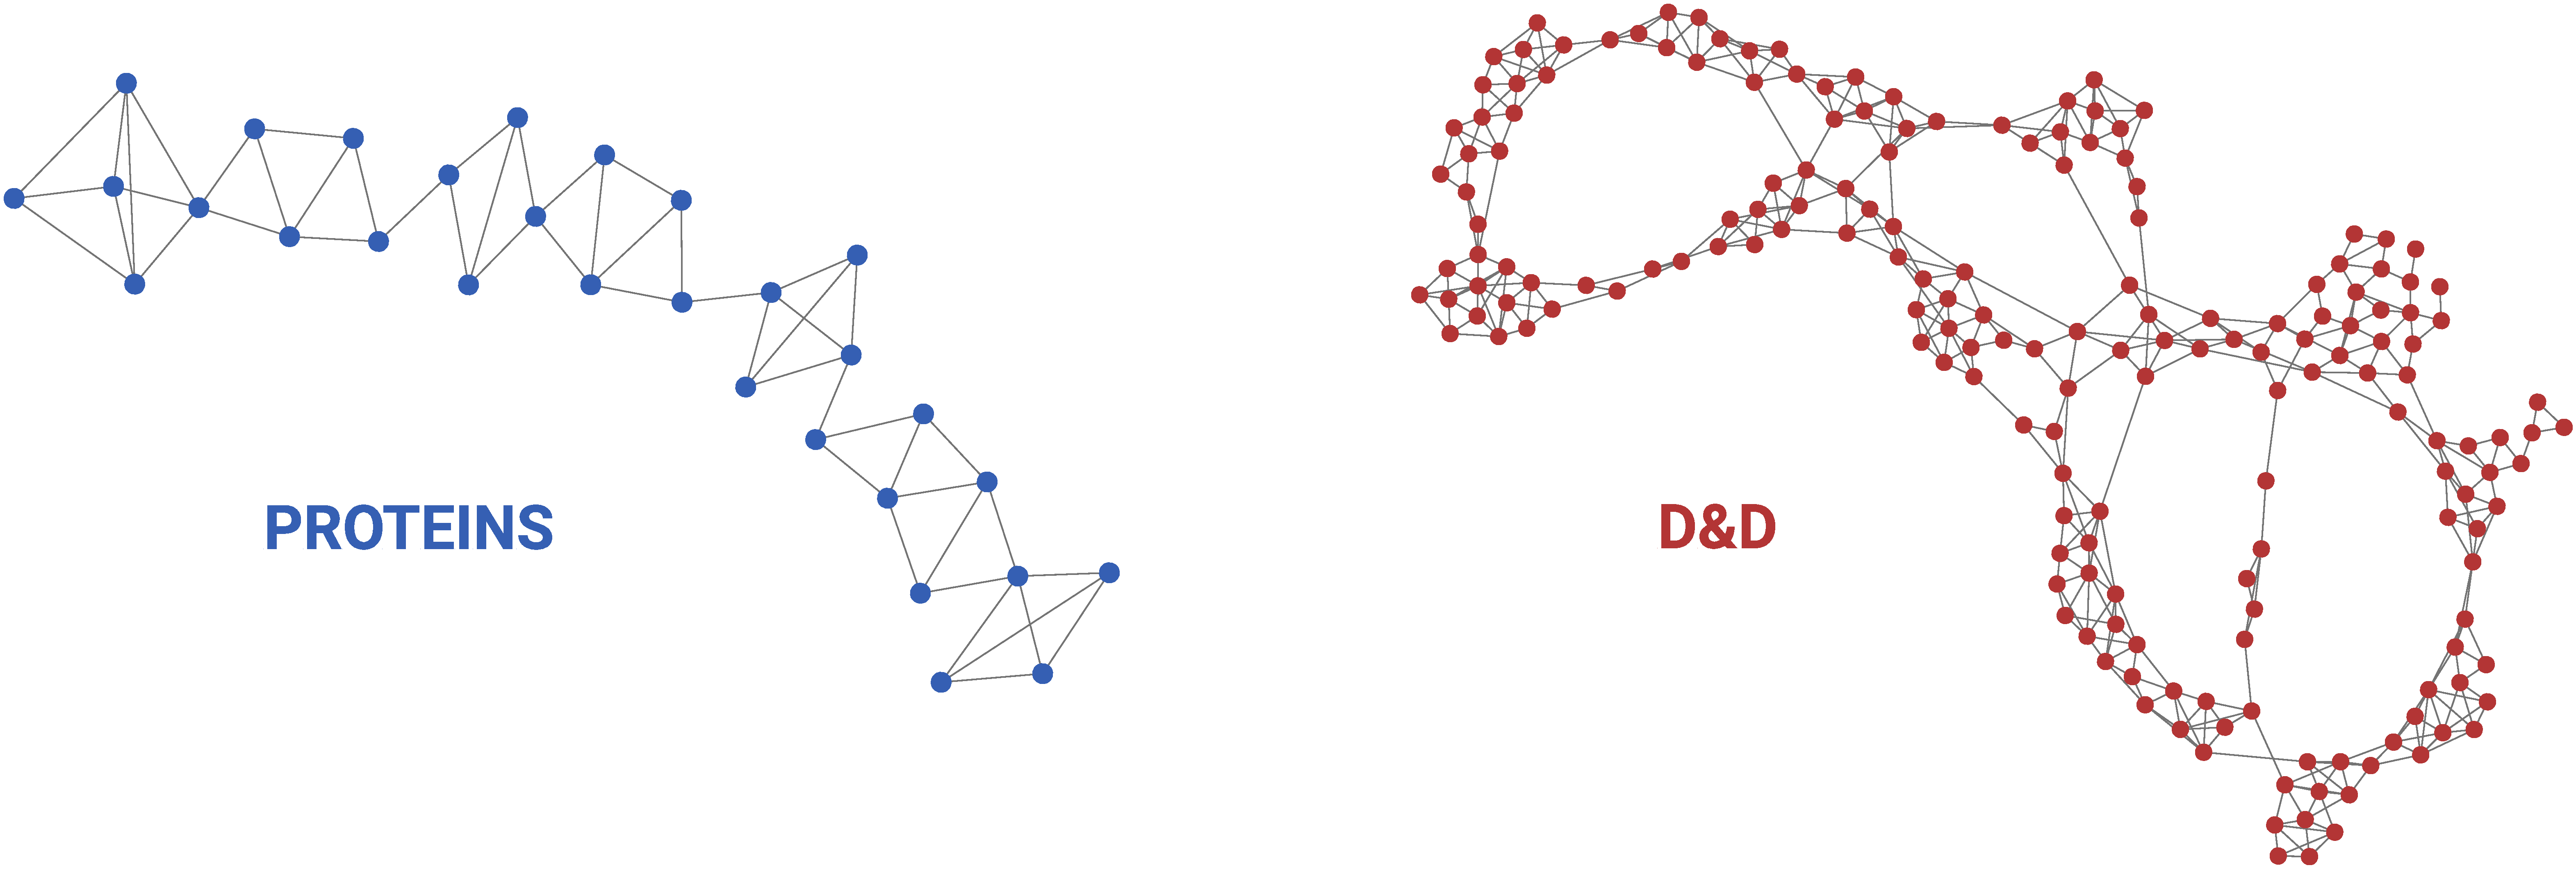
\includegraphics[width=0.8\linewidth]{gfx/evaluation/proteins-dd-diff.pdf}
	\caption{
		Two samples illustrating the difference between the PROTEINS and D\&D datasets.
	}\label{fig:evaluation:proteins-dd-diff}
\end{figure}

%!TEX root = ../main.tex
% chktex-file 46
\chapter{Conclusion}%
\label{sec:conclusion}

To conclude the thesis, we now look back on the three research questions described in \cref{sec:intro:questions} and summarize the answers we gave to them in the previous chapters.
Afterwards, a brief overview of future research directions based on our findings will be given.

\section{Review}%
\label{sec:conclusion:review}

\paragraph{\circled{1}\; What constitutes an \ac{lta} method?}
We began with a general definition of \ac{lta} in \cref{sec:ltag:definition}.
There we proposed that its defining characteristic should be the \textit{localized explainability} of its predictions.
This characteristic was formalized via the notion of \textit{\ac{lta} formulations} (see \cfullref{defn:ltag:formulation}) which requires that a model is expressible in terms of a decomposition function $\psi: \mathcal{G} \to \mathcal{P}(\mathcal{G})$, a local evaluation function $f: \mathcal{G} \to \mathcal{Y} \times \mathcal{R}$ and a weighted aggregation function $\mathcal{A}: {(\mathcal{Y} \times \mathcal{R}_{\geq 0})}^* \to \mathcal{Y}$.
An ideal \ac{lta} method has such a formulation with a decomposition function $\psi$ that splits graphs into ``meaningful'' constituents in some domain-specific sense of the word.
Since this ideal notion of \ac{lta} is generally quite fuzzy, we only distinguished between \acs{lta}-like and non-\acs{lta} methods in this thesis;
a method was called non-\acs{lta} if it uses a trivial decomposition function that just splits a graph $G$ into the single ``constituent'' $G$.

\paragraph{\circled{2}\; How do existing \ac{gcr} methods relate to \ac{lta}?}
In \cref{sec:ltag:formulation:svm,sec:ltag:formulation:gcnn} we used our definition of \ac{lta} to check which of the existing \ac{gcr} approaches are compatible with it.
For the case of an \ac{svm} using a graph kernel/embedding we found that it is an \acs{lta}-like method if the kernel is a so-called nontrivial \acf{sce} (see \cfullref{defn:ltag:substruct-embedding,thm:ltag:svm-ltag-formulation}).
This \ac{sce} condition is satisfied by fingerprint embeddings, the \ac{wl} subtree kernel and the 2-LWL kernel which makes them \acs{lta}-like.
However, \texttt{graph2vec} embeddings, the \ac{wl} shortest-path kernel and the 2-GWL kernel were found to be trivial or only partly nontrivial \acp{sce}, i.e.\ they are non-\acs{lta} methods.
After considering those embedding approaches we looked at \ac{gcnn} and showed that they also have an \ac{lta} formulation under certain conditions (see \cfullref{thm:ltag:gcnn-ltag-formulation}).
More specifically, we saw that the constituents used by a \ac{gcnn} are spanned by the \ac{bfs} subtrees of its input graph.

\paragraph{\circled{3}\; What are limitations of existing graph \ac{lta} methods and how can they be overcome?}
\Cref{sec:ltd:edge-filter} described that the subtree constituents are their primary limitation of \acp{gcnn} and that more flexible decompositions can be learned via an edge filtering strategy.
To realize edge filtering, we proposed that informative edge feature vectors could be used as the input to a filtering classifier.
To produce such feature vectors we first looked at 2-\acsp{gnn} and found that they have various theoretical limitations, i.e.\ the inability to distinguish regular graphs and to detect cycles (see \cfullref{prop:ltd:2gnn-regular-limit,prop:ltd:2gnn-cycle-limit}).
We therefore proposed the 2-\acs{wl}-\acs{gnn} which does not have those limitations (see \cfullref{cor:ltd:wl2-gnn-regular}).

\paragraph{Evaluation results}
For the evaluation of our results we considered two aspects:
Firstly, we looked at how 2-\acs{wl}-\acsp{gnn} compare to other \acp{gnn}.
Secondly, we evaluated how \acs{lta}-like methods compare to non-\acs{lta} methods.
Regarding the first aspect, we showed that the theoretical advantages of 2-\acs{wl}-\acsp{gnn} are clearly observable on the synthetic triangle detection dataset while on the evaluated real-world datasets we got results which are generally comparable with the best state-of-the-art approaches but not significantly better.
Regarding the second aspect, we observed no general advantage or disadvantage of \acs{lta}-like methods.
While the \acs{lta}-like configurations of 2-\acs{wl}-\acsp{gnn} generally performed worse than their non-\ac{lta} counterparts, the \acs{lta}-like \ac{wl} subtree kernel generally performed quite well.
This shows that \ac{lta} is in principle suitable for graph classification tasks if the right decomposition, evaluation and aggregation functions are chosen.

\section{Future Directions}%
\label{sec:conclusion:todo}


% --------------------------
% Back matter
% --------------------------
\appendix\cleardoublepage\
%!TEX root = ../main.tex
% chktex-file 46

\chapter{Appendix}%
\label{sec:appendix}

\section{Evaluated Hyperparameter Grids}%
\label{sec:appendix:config-grid}

To tune the hyperparameters of the evaluated models, we used a regular grid search.
Depending on the type of model, different sets of hyperparameter configurations $\Theta$ were used.

\paragraph{Graph Kernels}
As described in \cref{sec:eval:setup}, we used the \ac{svm} classifier from \citetitle{SKL} to evaluate the graph kernel approaches.
We tuned only the regularization parameter \texttt{C} of this classifier;
the evaluated values are $\mathtt{C} \in \{ 1, \num{1e-1},\allowbreak \num{1e-2},\allowbreak \num{1e-3},\allowbreak \num{1e-4} \}$.
All other parameters were left at the default setting (using \texttt{scikit-learn 0.22.1}).

\paragraph{Baseline and \ac{gin}}
For the evaluation of the structure unaware baseline learner and \ac{gin}, we used the same hyperparameter configurations as \citet{Errica2020}.
We therefore refer to their work for a complete list of the tuned hyperparameters for those models.

\paragraph{2-\acs{gnn} and 2-\acs{wl}-\acs{gnn}}
We evaluated our implementations of 2-\acsp{gnn} as well as 2-\acs{wl}-\acsp{gnn} on the grid spanned by the following hyperparameter values:
\begin{itemize}[itemsep=2pt,parsep=2pt]
	\item \textbf{Number of convolutional layers $T \in \{ 3, 5 \}$:}
		This parameter describes only the depth of the stack of convolutional layers.
		The \ac{mlp} after the pooling layer is always configured with a single hidden layer.
		The \acs{lta}-like configurations of 2-\acs{wl}-\acsp{gnn} are evaluated with the depths $T \in \{ 4, 5 \}$ to compensate for the missing \ac{mlp} after the pooling layer.
	\item \textbf{Layer width $d \in \{ 32, 64 \}$:}
		This parameter describes the output dimensionalities $d = d^{(1)} = \cdots = d^{(T)}$ of the convolutional layers and (if applicable) also the hidden layer width of the final \ac{mlp} after the pooling layer.
		The \acs{lta}-like configurations of 2-\acs{wl}-\acsp{gnn} are evaluated with the same widths but use $d^{(T)} = 1$ in the final layer.
	\item \textbf{Jumping knowledge $\mathrm{JK} \in \{ \mathtt{true}, \mathtt{false} \}$:}
		\citet{Xu2018a} have demonstrated that it can be advantageous for graph classification to pass the outputs of convolutional layers to their successors.
		We incorporate this idea by passing the input feature vectors not only to the first convolution layer but to all convolution layers through concatenation iff.\ $\mathrm{JK} = \mathtt{true}$.
	\item \textbf{Learning rate $\eta \in \{ \num{1e-2}, \num{1e-3}, \num{1e-4} \}$} of the Adam optimizer.
	\item \textbf{Activation functions $\sigma$ and $\sigma_{\Gamma}$} are set to the standard logistic function.
	\item \textbf{Number of epochs $E$ and early stopping patience $p$} are set to $E = 1000$ and $p = 100$, except for the evaluation of the synthetic TRIANGLE dataset for which we used $E = 5000$ and $p = 1000$ to ensure model convergence.
\end{itemize}

\section{Dataset Statistics and Descriptions}%
\label{sec:appendix:ds-stats}

\begin{table}[ht]
	\caption{Sizes of the evaluated binary classification datasets and their graphs.}\label{tbl:appendix:ds-stats}
	\centering\small
	\csvreader[
		tabular={lrrrrrrrrr},
		separator=comma,
		before reading=\setlength{\tabcolsep}{5pt},
		table head={%
			\multicolumn{1}{c}{} & \multicolumn{1}{c}{} & &\multicolumn{3}{c}{vertex count $\left|\mathcal{V}_G\right|$} & \multicolumn{3}{c}{edge count $\left|\mathcal{E}_G\right|$} & \multicolumn{1}{c}{radius} \\%
			& \multirow{-2}{*}[-0.2em]{\shortstack[c]{no.\ of\\ graphs}} & \multirow{-2}{*}[-0.2em]{\shortstack[c]{vertex data\\{\scriptsize (feat.\ + lab.)}}} & $\min$ & $\mean$ & $\max$ & $\min$ & $\mean$ & $\max$ & $\mean \pm\, \sigma$ \\\toprule% chktex 21
		},
		table foot=\bottomrule,
		late after line=\\
	]{data/ds_stats.csv}%
	{name=\name,graph_count=\gcount,%
	node_count_min=\ncountmin,node_count_mean=\ncountmean,node_count_max=\ncountmax,%
	edge_count_min=\ecountmin,edge_count_mean=\ecountmean,edge_count_max=\ecountmax,%
	node_degree_min=\ndegmin,node_degree_mean=\ndegmean,node_degree_max=\ndegmax,%
	dim_node_features=\nfdim,dim_edge_features=\efdim, radius_mean=\radiusmean, radius_std=\radiusstd%
	}%
	{\textbf{\name}&%
	$\gcount$&%
	$\nfdim$&%
	$\ncountmin$&$\ncountmean$&$\ncountmax$&%
	$\ecountmin$&$\ecountmean$&$\ecountmax$&$\radiusmean \pm \radiusstd$%
	}
\end{table}

\paragraph{TRIANGLE}
The triangle detection dataset was generated by sampling three graphs with exactly one unicolored triangle uniformly at random for each possible combination of the following parameters:
The number of vertices (between 6 and 32), the vertex color proportions (either 50/50\%, 75/25\% or 25/75\% vertices with the colors \colorlabel{t_blue}{A}/\colorlabel{t_red}{B}), the graph density (${\left| \mathcal{V}_{G} \right|}^{-2} \left| \mathcal{E}_{G} \right| \in \{ \nicefrac{1}{4}, \nicefrac{1}{2} \}$) the graph class (add a triangle with either the color \colorlabel{t_blue}{A} or \colorlabel{t_red}{B}).

\paragraph{NCI1}
This dataset was made available by \citet{Shervashidze2011}.
It contains a balanced subset of molecule graphs that were originally published by the US \ac{nci}~\cite{Wale2007}.
In each molecule graph, vertices correspond to atoms and edges to bonds between them.
The binary classes in this dataset describe whether a molecule is able to suppress or inhibit the growth of certain lung cancer and ovarian cancer cell lines in humans.

\paragraph{PROTEINS and D\&D}
The graphs in both the PROTEINS dataset~\cite{Borgwardt2005a} as well as the D\&D dataset~\cite{Dobson2003} represent proteins.
Each vertex corresponds to a so-called \ac{sse}, i.e.\ a certain molecular substructure.
An edge encodes either that two \acp{sse} are neighbors in the protein's amino-acid sequence or that those \acp{sse} are close to each other in 3D space.
Each protein graph is classified by whether it is an enzyme or not.
The main difference between the two datasets is their selection of vertex features/labels.

\paragraph{REDDIT}
This balanced dataset contains graphs that represent online discussion threads on the website Reddit~\cite{Yanardag2015}.
Each vertex corresponds to a user; an edge is drawn between two users iff.\ at least one of them replied to a comment of another.
Such social interaction graphs were sampled from two types of subreddits:
Question/answer-based and discussion-based.
The classification goal is to predict from which type of subreddit a given graph was sampled.

\paragraph{IMDB}
This dataset contains so-called \textit{ego-networks} of movie actors~\cite{Yanardag2015}.
Vertices in such networks represent actors and edges encode whether two actors starred in the same movie.
The graphs in the dataset are derived from the actors starring in either action or romance movies.
The classification goal for each graph is to predict the movie genre it was derived from.

\section{Fold-wise Accuracy Deltas}%
\label{sec:appendix:fold-diffs}

Due to the relatively small sizes of the evaluated benchmark datasets, the variance of the test accuracies across different folds is quite large.
When directly comparing the mean accuracies of two learners, it is therefore often impossible to tell whether one consistently outperforms the other.
We therefore now list the mean and standard deviations of the fold-wise test accuracy differences of all pairs of learners for all datasets.
This effectively removes the variance introduced by ``easy'' and ``hard'' folds on which all learners might tend to perform consistently better/worse.

In the following \crefrange{tbl:appendix:diff-triangle}{tbl:appendix:diff-imdb} (\cpagerefrange{tbl:appendix:diff-triangle}{tbl:appendix:diff-imdb}), we show accuracy differences as $\textit{row accuracy} - \textit{column accuracy}$.
For each row $i$ and column $j$ the corresponding cell $(i,j)$ is highlighted in \textcolor{t_red}{red} or \textcolor{t_darkgreen}{green} iff.\ the learner~$i$ performs consistently \textcolor{t_red}{worse} (or \textcolor{t_darkgreen}{better} respectively) than $j$ with a significance level of $2\sigma$.
To compute the deltas for 2-\acs{wl}-\acsp{gnn}, the same neighborhood radii as in \cref{tbl:eval:synthetic,tbl:eval:real} are used, i.e.\ $r = 2$ for the synthetic triangle detection dataset and $r = 8$, $5$, $2$, $1$ and $4$ for NCI1, PROTEINS, D\&D, REDDIT and IMDB respectively.

{\captionsetup[table]{name=Matrix}%
\begin{table}[ht]
	\caption{Fold-wise accuracy delta means and standard deviations on the triangle dataset.}\label[mat]{tbl:appendix:diff-triangle}
	\centering
	% This file was generated by the LTAG results postprocessor. Do not edit manually.
{\setlength\tabcolsep{2.5pt}\setlength{\extrarowheight}{2pt}%
\begin{tabular}{lcccccccccccc}
& \rotatebox[origin=l]{90}{\textbf{\textcolor{t_darkgreen}{WL\textsubscript{ST}*}} ($T=3$)} & \rotatebox[origin=l]{90}{\textbf{WL\textsubscript{SP}} ($T=3$)} & \rotatebox[origin=l]{90}{\textbf{\textcolor{t_darkgreen}{2-LWL*}} ($T=3$)} & \rotatebox[origin=l]{90}{\textbf{2-GWL} ($T=3$)} & \rotatebox[origin=l]{90}{\textbf{Baseline} ($\mathrm{sum}$)} & \rotatebox[origin=l]{90}{\textbf{GIN} ($\mathrm{sum}$)} & \rotatebox[origin=l]{90}{\textbf{2-GNN} ($\mean$)} & \rotatebox[origin=l]{90}{\textbf{2-GNN} ($\mathrm{SAM}$)} & \rotatebox[origin=l]{90}{\textbf{\textcolor{t_darkgreen}{2-WL-GNN*}} ($\mean$)} & \rotatebox[origin=l]{90}{\textbf{2-WL-GNN\phantom{*}} ($\mean$)} & \rotatebox[origin=l]{90}{\textbf{\textcolor{t_darkgreen}{2-WL-GNN*}} ($\mathrm{SAM}$)} & \rotatebox[origin=l]{90}{\textbf{2-WL-GNN\phantom{*}} ($\mathrm{SAM}$)} \\
\textbf{\textcolor{t_darkgreen}{WL\textsubscript{ST}*}} ($T=3$)& & {\tiny\Vectorstack{-11\\ \pm 13}} & {\tiny\Vectorstack{+0.4\\ \pm 9.6}} & {\tiny\Vectorstack{-4.9\\ \pm 16}} & {\tiny\Vectorstack{+12\\ \pm 12}} & {\tiny\Vectorstack{-13\\ \pm 10}} & {\tiny\Vectorstack{-20\\ \pm 14}} & {\tiny\Vectorstack{-25\\ \pm 14}} & \cellcolor{t_red!25}\textcolor{t_darkred}{{\tiny\Vectorstack{-34\\ \pm 14}}} & \cellcolor{t_red!25}\textcolor{t_darkred}{{\tiny\Vectorstack{-36\\ \pm 17}}} & \cellcolor{t_red!25}\textcolor{t_darkred}{{\tiny\Vectorstack{-34\\ \pm 8.6}}} & \cellcolor{t_red!25}\textcolor{t_darkred}{{\tiny\Vectorstack{-42\\ \pm 11}}} \\[2pt]
\textbf{WL\textsubscript{SP}} ($T=3$)&{\tiny\Vectorstack{+11\\ \pm 13}} &  & {\tiny\Vectorstack{+11\\ \pm 13}} & {\tiny\Vectorstack{+6.1\\ \pm 9.2}} & {\tiny\Vectorstack{+23\\ \pm 16}} & {\tiny\Vectorstack{-2.0\\ \pm 14}} & {\tiny\Vectorstack{-8.8\\ \pm 13}} & {\tiny\Vectorstack{-14\\ \pm 14}} & \cellcolor{t_red!25}\textcolor{t_darkred}{{\tiny\Vectorstack{-23\\ \pm 11}}} & \cellcolor{t_red!25}\textcolor{t_darkred}{{\tiny\Vectorstack{-25\\ \pm 12}}} & \cellcolor{t_red!25}\textcolor{t_darkred}{{\tiny\Vectorstack{-23\\ \pm 8.4}}} & \cellcolor{t_red!25}\textcolor{t_darkred}{{\tiny\Vectorstack{-31\\ \pm 11}}} \\[2pt]
\textbf{\textcolor{t_darkgreen}{2-LWL*}} ($T=3$)&{\tiny\Vectorstack{-0.4\\ \pm 9.6}} & {\tiny\Vectorstack{-11\\ \pm 13}} &  & {\tiny\Vectorstack{-5.3\\ \pm 11}} & {\tiny\Vectorstack{+12\\ \pm 7.5}} & {\tiny\Vectorstack{-13\\ \pm 6.7}} & {\tiny\Vectorstack{-20\\ \pm 13}} & \cellcolor{t_red!25}\textcolor{t_darkred}{{\tiny\Vectorstack{-25\\ \pm 9.4}}} & \cellcolor{t_red!25}\textcolor{t_darkred}{{\tiny\Vectorstack{-34\\ \pm 8.6}}} & \cellcolor{t_red!25}\textcolor{t_darkred}{{\tiny\Vectorstack{-36\\ \pm 10}}} & \cellcolor{t_red!25}\textcolor{t_darkred}{{\tiny\Vectorstack{-34\\ \pm 7.0}}} & \cellcolor{t_red!25}\textcolor{t_darkred}{{\tiny\Vectorstack{-43\\ \pm 6.8}}} \\[2pt]
\textbf{2-GWL} ($T=3$)&{\tiny\Vectorstack{+4.9\\ \pm 16}} & {\tiny\Vectorstack{-6.1\\ \pm 9.2}} & {\tiny\Vectorstack{+5.3\\ \pm 11}} &  & {\tiny\Vectorstack{+17\\ \pm 15}} & {\tiny\Vectorstack{-8.2\\ \pm 13}} & {\tiny\Vectorstack{-15\\ \pm 14}} & {\tiny\Vectorstack{-20\\ \pm 13}} & \cellcolor{t_red!25}\textcolor{t_darkred}{{\tiny\Vectorstack{-29\\ \pm 8.8}}} & \cellcolor{t_red!25}\textcolor{t_darkred}{{\tiny\Vectorstack{-31\\ \pm 9.0}}} & \cellcolor{t_red!25}\textcolor{t_darkred}{{\tiny\Vectorstack{-29\\ \pm 10}}} & \cellcolor{t_red!25}\textcolor{t_darkred}{{\tiny\Vectorstack{-38\\ \pm 9.0}}} \\[2pt]
\textbf{Baseline} ($\mathrm{sum}$)&{\tiny\Vectorstack{-12\\ \pm 12}} & {\tiny\Vectorstack{-23\\ \pm 16}} & {\tiny\Vectorstack{-12\\ \pm 7.5}} & {\tiny\Vectorstack{-17\\ \pm 15}} &  & \cellcolor{t_red!25}\textcolor{t_darkred}{{\tiny\Vectorstack{-25\\ \pm 8.4}}} & \cellcolor{t_red!25}\textcolor{t_darkred}{{\tiny\Vectorstack{-32\\ \pm 14}}} & \cellcolor{t_red!25}\textcolor{t_darkred}{{\tiny\Vectorstack{-37\\ \pm 9.2}}} & \cellcolor{t_red!25}\textcolor{t_darkred}{{\tiny\Vectorstack{-46\\ \pm 9.8}}} & \cellcolor{t_red!25}\textcolor{t_darkred}{{\tiny\Vectorstack{-48\\ \pm 14}}} & \cellcolor{t_red!25}\textcolor{t_darkred}{{\tiny\Vectorstack{-46\\ \pm 9.2}}} & \cellcolor{t_red!25}\textcolor{t_darkred}{{\tiny\Vectorstack{-55\\ \pm 8.5}}} \\[2pt]
\textbf{GIN} ($\mathrm{sum}$)&{\tiny\Vectorstack{+13\\ \pm 10}} & {\tiny\Vectorstack{+2.0\\ \pm 14}} & {\tiny\Vectorstack{+13\\ \pm 6.7}} & {\tiny\Vectorstack{+8.2\\ \pm 13}} & \cellcolor{t_green!25}\textcolor{t_darkgreen}{{\tiny\Vectorstack{+25\\ \pm 8.4}}} &  & {\tiny\Vectorstack{-6.8\\ \pm 13}} & {\tiny\Vectorstack{-12\\ \pm 9.5}} & \cellcolor{t_red!25}\textcolor{t_darkred}{{\tiny\Vectorstack{-21\\ \pm 9.9}}} & {\tiny\Vectorstack{-23\\ \pm 14}} & \cellcolor{t_red!25}\textcolor{t_darkred}{{\tiny\Vectorstack{-21\\ \pm 8.3}}} & \cellcolor{t_red!25}\textcolor{t_darkred}{{\tiny\Vectorstack{-29\\ \pm 7.3}}} \\[2pt]
\textbf{2-GNN} ($\mean$)&{\tiny\Vectorstack{+20\\ \pm 14}} & {\tiny\Vectorstack{+8.8\\ \pm 13}} & {\tiny\Vectorstack{+20\\ \pm 13}} & {\tiny\Vectorstack{+15\\ \pm 14}} & \cellcolor{t_green!25}\textcolor{t_darkgreen}{{\tiny\Vectorstack{+32\\ \pm 14}}} & {\tiny\Vectorstack{+6.8\\ \pm 13}} &  & {\tiny\Vectorstack{-5.0\\ \pm 6.6}} & {\tiny\Vectorstack{-14\\ \pm 9.6}} & {\tiny\Vectorstack{-16\\ \pm 11}} & {\tiny\Vectorstack{-14\\ \pm 8.8}} & \cellcolor{t_red!25}\textcolor{t_darkred}{{\tiny\Vectorstack{-23\\ \pm 9.8}}} \\[2pt]
\textbf{2-GNN} ($\mathrm{SAM}$)&{\tiny\Vectorstack{+25\\ \pm 14}} & {\tiny\Vectorstack{+14\\ \pm 14}} & \cellcolor{t_green!25}\textcolor{t_darkgreen}{{\tiny\Vectorstack{+25\\ \pm 9.4}}} & {\tiny\Vectorstack{+20\\ \pm 13}} & \cellcolor{t_green!25}\textcolor{t_darkgreen}{{\tiny\Vectorstack{+37\\ \pm 9.2}}} & {\tiny\Vectorstack{+12\\ \pm 9.5}} & {\tiny\Vectorstack{+5.0\\ \pm 6.6}} &  & {\tiny\Vectorstack{-8.9\\ \pm 6.3}} & {\tiny\Vectorstack{-11\\ \pm 8.8}} & {\tiny\Vectorstack{-9.2\\ \pm 7.1}} & \cellcolor{t_red!25}\textcolor{t_darkred}{{\tiny\Vectorstack{-18\\ \pm 7.2}}} \\[2pt]
\textbf{\textcolor{t_darkgreen}{2-WL-GNN*}} ($\mean$)&\cellcolor{t_green!25}\textcolor{t_darkgreen}{{\tiny\Vectorstack{+34\\ \pm 14}}} & \cellcolor{t_green!25}\textcolor{t_darkgreen}{{\tiny\Vectorstack{+23\\ \pm 11}}} & \cellcolor{t_green!25}\textcolor{t_darkgreen}{{\tiny\Vectorstack{+34\\ \pm 8.6}}} & \cellcolor{t_green!25}\textcolor{t_darkgreen}{{\tiny\Vectorstack{+29\\ \pm 8.8}}} & \cellcolor{t_green!25}\textcolor{t_darkgreen}{{\tiny\Vectorstack{+46\\ \pm 9.8}}} & \cellcolor{t_green!25}\textcolor{t_darkgreen}{{\tiny\Vectorstack{+21\\ \pm 9.9}}} & {\tiny\Vectorstack{+14\\ \pm 9.6}} & {\tiny\Vectorstack{+8.9\\ \pm 6.3}} &  & {\tiny\Vectorstack{-2.2\\ \pm 7.2}} & {\tiny\Vectorstack{-0.3\\ \pm 6.0}} & {\tiny\Vectorstack{-8.7\\ \pm 4.6}} \\[2pt]
\textbf{2-WL-GNN\phantom{*}} ($\mean$)&\cellcolor{t_green!25}\textcolor{t_darkgreen}{{\tiny\Vectorstack{+36\\ \pm 17}}} & \cellcolor{t_green!25}\textcolor{t_darkgreen}{{\tiny\Vectorstack{+25\\ \pm 12}}} & \cellcolor{t_green!25}\textcolor{t_darkgreen}{{\tiny\Vectorstack{+36\\ \pm 10}}} & \cellcolor{t_green!25}\textcolor{t_darkgreen}{{\tiny\Vectorstack{+31\\ \pm 9.0}}} & \cellcolor{t_green!25}\textcolor{t_darkgreen}{{\tiny\Vectorstack{+48\\ \pm 14}}} & {\tiny\Vectorstack{+23\\ \pm 14}} & {\tiny\Vectorstack{+16\\ \pm 11}} & {\tiny\Vectorstack{+11\\ \pm 8.8}} & {\tiny\Vectorstack{+2.2\\ \pm 7.2}} &  & {\tiny\Vectorstack{+1.9\\ \pm 9.7}} & {\tiny\Vectorstack{-6.5\\ \pm 8.7}} \\[2pt]
\textbf{\textcolor{t_darkgreen}{2-WL-GNN*}} ($\mathrm{SAM}$)&\cellcolor{t_green!25}\textcolor{t_darkgreen}{{\tiny\Vectorstack{+34\\ \pm 8.6}}} & \cellcolor{t_green!25}\textcolor{t_darkgreen}{{\tiny\Vectorstack{+23\\ \pm 8.4}}} & \cellcolor{t_green!25}\textcolor{t_darkgreen}{{\tiny\Vectorstack{+34\\ \pm 7.0}}} & \cellcolor{t_green!25}\textcolor{t_darkgreen}{{\tiny\Vectorstack{+29\\ \pm 10}}} & \cellcolor{t_green!25}\textcolor{t_darkgreen}{{\tiny\Vectorstack{+46\\ \pm 9.2}}} & \cellcolor{t_green!25}\textcolor{t_darkgreen}{{\tiny\Vectorstack{+21\\ \pm 8.3}}} & {\tiny\Vectorstack{+14\\ \pm 8.8}} & {\tiny\Vectorstack{+9.2\\ \pm 7.1}} & {\tiny\Vectorstack{+0.3\\ \pm 6.0}} & {\tiny\Vectorstack{-1.9\\ \pm 9.7}} &  & {\tiny\Vectorstack{-8.5\\ \pm 4.7}} \\[2pt]
\textbf{2-WL-GNN\phantom{*}} ($\mathrm{SAM}$)&\cellcolor{t_green!25}\textcolor{t_darkgreen}{{\tiny\Vectorstack{+42\\ \pm 11}}} & \cellcolor{t_green!25}\textcolor{t_darkgreen}{{\tiny\Vectorstack{+31\\ \pm 11}}} & \cellcolor{t_green!25}\textcolor{t_darkgreen}{{\tiny\Vectorstack{+43\\ \pm 6.8}}} & \cellcolor{t_green!25}\textcolor{t_darkgreen}{{\tiny\Vectorstack{+38\\ \pm 9.0}}} & \cellcolor{t_green!25}\textcolor{t_darkgreen}{{\tiny\Vectorstack{+55\\ \pm 8.5}}} & \cellcolor{t_green!25}\textcolor{t_darkgreen}{{\tiny\Vectorstack{+29\\ \pm 7.3}}} & \cellcolor{t_green!25}\textcolor{t_darkgreen}{{\tiny\Vectorstack{+23\\ \pm 9.8}}} & \cellcolor{t_green!25}\textcolor{t_darkgreen}{{\tiny\Vectorstack{+18\\ \pm 7.2}}} & {\tiny\Vectorstack{+8.7\\ \pm 4.6}} & {\tiny\Vectorstack{+6.5\\ \pm 8.7}} & {\tiny\Vectorstack{+8.5\\ \pm 4.7}} & 
\end{tabular}}

\end{table}
\begin{table}[ht]
	\caption{Fold-wise accuracy delta means and standard deviations on NCI1.}\label[mat]{tbl:appendix:diff-nci}
	\centering
	% This file was generated by the LTAG results postprocessor. Do not edit manually.
{\setlength\tabcolsep{2.5pt}\setlength{\extrarowheight}{2pt}%
\begin{tabular}{lcccccccccccc}
& \rotatebox[origin=l]{90}{\textbf{\textcolor{t_darkgreen}{WL\textsubscript{ST}*}} ($T=1$)} & \rotatebox[origin=l]{90}{\textbf{\textcolor{t_darkgreen}{WL\textsubscript{ST}*}} ($T=3$)} & \rotatebox[origin=l]{90}{\textbf{\textcolor{t_darkgreen}{2-LWL*}} ($T=3$)} & \rotatebox[origin=l]{90}{\textbf{2-GWL} ($T=3$)} & \rotatebox[origin=l]{90}{\textbf{Baseline} ($\mathrm{sum}$)} & \rotatebox[origin=l]{90}{\textbf{GIN} ($\mathrm{sum}$)} & \rotatebox[origin=l]{90}{\textbf{2-GNN} ($\mean$)} & \rotatebox[origin=l]{90}{\textbf{2-GNN} ($\mathrm{SAM}$)} & \rotatebox[origin=l]{90}{\textbf{\textcolor{t_darkgreen}{2-WL-GNN*}} ($\mean$)} & \rotatebox[origin=l]{90}{\textbf{2-WL-GNN\phantom{*}} ($\mean$)} & \rotatebox[origin=l]{90}{\textbf{\textcolor{t_darkgreen}{2-WL-GNN*}} ($\mathrm{SAM}$)} & \rotatebox[origin=l]{90}{\textbf{2-WL-GNN\phantom{*}} ($\mathrm{SAM}$)} \\
\textbf{\textcolor{t_darkgreen}{WL\textsubscript{ST}*}} ($T=1$)& & \cellcolor{t_red!25}\textcolor{t_darkred}{{\tiny\Vectorstack{-11\\ \pm 1.3}}} & {\tiny\Vectorstack{-2.8\\ \pm 1.5}} & {\tiny\Vectorstack{+2.3\\ \pm 2.4}} & \cellcolor{t_green!25}\textcolor{t_darkgreen}{{\tiny\Vectorstack{+6.2\\ \pm 2.9}}} & {\tiny\Vectorstack{-3.5\\ \pm 2.2}} & {\tiny\Vectorstack{-1.9\\ \pm 2.9}} & {\tiny\Vectorstack{-4.4\\ \pm 2.3}} & {\tiny\Vectorstack{+3.1\\ \pm 2.5}} & {\tiny\Vectorstack{+1.6\\ \pm 2.6}} & {\tiny\Vectorstack{+3.7\\ \pm 3.6}} & {\tiny\Vectorstack{+0.4\\ \pm 2.1}} \\[2pt]
\textbf{\textcolor{t_darkgreen}{WL\textsubscript{ST}*}} ($T=3$)&\cellcolor{t_green!25}\textcolor{t_darkgreen}{{\tiny\Vectorstack{+11\\ \pm 1.3}}} &  & \cellcolor{t_green!25}\textcolor{t_darkgreen}{{\tiny\Vectorstack{+8.1\\ \pm 1.6}}} & \cellcolor{t_green!25}\textcolor{t_darkgreen}{{\tiny\Vectorstack{+13\\ \pm 1.8}}} & \cellcolor{t_green!25}\textcolor{t_darkgreen}{{\tiny\Vectorstack{+17\\ \pm 2.9}}} & \cellcolor{t_green!25}\textcolor{t_darkgreen}{{\tiny\Vectorstack{+7.3\\ \pm 2.7}}} & \cellcolor{t_green!25}\textcolor{t_darkgreen}{{\tiny\Vectorstack{+8.9\\ \pm 2.3}}} & \cellcolor{t_green!25}\textcolor{t_darkgreen}{{\tiny\Vectorstack{+6.5\\ \pm 2.0}}} & \cellcolor{t_green!25}\textcolor{t_darkgreen}{{\tiny\Vectorstack{+14\\ \pm 2.8}}} & \cellcolor{t_green!25}\textcolor{t_darkgreen}{{\tiny\Vectorstack{+12\\ \pm 2.5}}} & \cellcolor{t_green!25}\textcolor{t_darkgreen}{{\tiny\Vectorstack{+15\\ \pm 4.2}}} & \cellcolor{t_green!25}\textcolor{t_darkgreen}{{\tiny\Vectorstack{+11\\ \pm 2.0}}} \\[2pt]
\textbf{\textcolor{t_darkgreen}{2-LWL*}} ($T=3$)&{\tiny\Vectorstack{+2.8\\ \pm 1.5}} & \cellcolor{t_red!25}\textcolor{t_darkred}{{\tiny\Vectorstack{-8.1\\ \pm 1.6}}} &  & \cellcolor{t_green!25}\textcolor{t_darkgreen}{{\tiny\Vectorstack{+5.1\\ \pm 2.3}}} & \cellcolor{t_green!25}\textcolor{t_darkgreen}{{\tiny\Vectorstack{+9.0\\ \pm 3.0}}} & {\tiny\Vectorstack{-0.7\\ \pm 2.7}} & {\tiny\Vectorstack{+0.9\\ \pm 2.0}} & {\tiny\Vectorstack{-1.6\\ \pm 2.3}} & {\tiny\Vectorstack{+5.9\\ \pm 3.2}} & {\tiny\Vectorstack{+4.4\\ \pm 2.5}} & {\tiny\Vectorstack{+6.5\\ \pm 4.2}} & {\tiny\Vectorstack{+3.2\\ \pm 2.5}} \\[2pt]
\textbf{2-GWL} ($T=3$)&{\tiny\Vectorstack{-2.3\\ \pm 2.4}} & \cellcolor{t_red!25}\textcolor{t_darkred}{{\tiny\Vectorstack{-13\\ \pm 1.8}}} & \cellcolor{t_red!25}\textcolor{t_darkred}{{\tiny\Vectorstack{-5.1\\ \pm 2.3}}} &  & {\tiny\Vectorstack{+3.9\\ \pm 4.1}} & {\tiny\Vectorstack{-5.8\\ \pm 3.6}} & {\tiny\Vectorstack{-4.3\\ \pm 2.5}} & \cellcolor{t_red!25}\textcolor{t_darkred}{{\tiny\Vectorstack{-6.7\\ \pm 2.5}}} & {\tiny\Vectorstack{+0.8\\ \pm 3.7}} & {\tiny\Vectorstack{-0.8\\ \pm 2.7}} & {\tiny\Vectorstack{+1.4\\ \pm 4.0}} & {\tiny\Vectorstack{-1.9\\ \pm 3.1}} \\[2pt]
\textbf{Baseline} ($\mathrm{sum}$)&\cellcolor{t_red!25}\textcolor{t_darkred}{{\tiny\Vectorstack{-6.2\\ \pm 2.9}}} & \cellcolor{t_red!25}\textcolor{t_darkred}{{\tiny\Vectorstack{-17\\ \pm 2.9}}} & \cellcolor{t_red!25}\textcolor{t_darkred}{{\tiny\Vectorstack{-9.0\\ \pm 3.0}}} & {\tiny\Vectorstack{-3.9\\ \pm 4.1}} &  & \cellcolor{t_red!25}\textcolor{t_darkred}{{\tiny\Vectorstack{-9.8\\ \pm 2.4}}} & \cellcolor{t_red!25}\textcolor{t_darkred}{{\tiny\Vectorstack{-8.2\\ \pm 2.9}}} & \cellcolor{t_red!25}\textcolor{t_darkred}{{\tiny\Vectorstack{-11\\ \pm 2.6}}} & {\tiny\Vectorstack{-3.1\\ \pm 3.0}} & {\tiny\Vectorstack{-4.7\\ \pm 3.1}} & {\tiny\Vectorstack{-2.6\\ \pm 5.0}} & \cellcolor{t_red!25}\textcolor{t_darkred}{{\tiny\Vectorstack{-5.8\\ \pm 2.8}}} \\[2pt]
\textbf{GIN} ($\mathrm{sum}$)&{\tiny\Vectorstack{+3.5\\ \pm 2.2}} & \cellcolor{t_red!25}\textcolor{t_darkred}{{\tiny\Vectorstack{-7.3\\ \pm 2.7}}} & {\tiny\Vectorstack{+0.7\\ \pm 2.7}} & {\tiny\Vectorstack{+5.8\\ \pm 3.6}} & \cellcolor{t_green!25}\textcolor{t_darkgreen}{{\tiny\Vectorstack{+9.8\\ \pm 2.4}}} &  & {\tiny\Vectorstack{+1.6\\ \pm 3.5}} & {\tiny\Vectorstack{-0.9\\ \pm 2.2}} & \cellcolor{t_green!25}\textcolor{t_darkgreen}{{\tiny\Vectorstack{+6.6\\ \pm 2.5}}} & {\tiny\Vectorstack{+5.1\\ \pm 3.2}} & \cellcolor{t_green!25}\textcolor{t_darkgreen}{{\tiny\Vectorstack{+7.2\\ \pm 3.3}}} & {\tiny\Vectorstack{+3.9\\ \pm 3.3}} \\[2pt]
\textbf{2-GNN} ($\mean$)&{\tiny\Vectorstack{+1.9\\ \pm 2.9}} & \cellcolor{t_red!25}\textcolor{t_darkred}{{\tiny\Vectorstack{-8.9\\ \pm 2.3}}} & {\tiny\Vectorstack{-0.9\\ \pm 2.0}} & {\tiny\Vectorstack{+4.3\\ \pm 2.5}} & \cellcolor{t_green!25}\textcolor{t_darkgreen}{{\tiny\Vectorstack{+8.2\\ \pm 2.9}}} & {\tiny\Vectorstack{-1.6\\ \pm 3.5}} &  & {\tiny\Vectorstack{-2.4\\ \pm 2.6}} & {\tiny\Vectorstack{+5.1\\ \pm 3.5}} & {\tiny\Vectorstack{+3.5\\ \pm 2.2}} & {\tiny\Vectorstack{+5.6\\ \pm 4.8}} & {\tiny\Vectorstack{+2.4\\ \pm 2.6}} \\[2pt]
\textbf{2-GNN} ($\mathrm{SAM}$)&{\tiny\Vectorstack{+4.4\\ \pm 2.3}} & \cellcolor{t_red!25}\textcolor{t_darkred}{{\tiny\Vectorstack{-6.5\\ \pm 2.0}}} & {\tiny\Vectorstack{+1.6\\ \pm 2.3}} & \cellcolor{t_green!25}\textcolor{t_darkgreen}{{\tiny\Vectorstack{+6.7\\ \pm 2.5}}} & \cellcolor{t_green!25}\textcolor{t_darkgreen}{{\tiny\Vectorstack{+11\\ \pm 2.6}}} & {\tiny\Vectorstack{+0.9\\ \pm 2.2}} & {\tiny\Vectorstack{+2.4\\ \pm 2.6}} &  & \cellcolor{t_green!25}\textcolor{t_darkgreen}{{\tiny\Vectorstack{+7.5\\ \pm 3.1}}} & {\tiny\Vectorstack{+5.9\\ \pm 3.2}} & {\tiny\Vectorstack{+8.1\\ \pm 4.2}} & {\tiny\Vectorstack{+4.8\\ \pm 3.2}} \\[2pt]
\textbf{\textcolor{t_darkgreen}{2-WL-GNN*}} ($\mean$)&{\tiny\Vectorstack{-3.1\\ \pm 2.5}} & \cellcolor{t_red!25}\textcolor{t_darkred}{{\tiny\Vectorstack{-14\\ \pm 2.8}}} & {\tiny\Vectorstack{-5.9\\ \pm 3.2}} & {\tiny\Vectorstack{-0.8\\ \pm 3.7}} & {\tiny\Vectorstack{+3.1\\ \pm 3.0}} & \cellcolor{t_red!25}\textcolor{t_darkred}{{\tiny\Vectorstack{-6.6\\ \pm 2.5}}} & {\tiny\Vectorstack{-5.1\\ \pm 3.5}} & \cellcolor{t_red!25}\textcolor{t_darkred}{{\tiny\Vectorstack{-7.5\\ \pm 3.1}}} &  & {\tiny\Vectorstack{-1.5\\ \pm 2.2}} & {\tiny\Vectorstack{+0.6\\ \pm 2.9}} & {\tiny\Vectorstack{-2.7\\ \pm 2.3}} \\[2pt]
\textbf{2-WL-GNN\phantom{*}} ($\mean$)&{\tiny\Vectorstack{-1.6\\ \pm 2.6}} & \cellcolor{t_red!25}\textcolor{t_darkred}{{\tiny\Vectorstack{-12\\ \pm 2.5}}} & {\tiny\Vectorstack{-4.4\\ \pm 2.5}} & {\tiny\Vectorstack{+0.8\\ \pm 2.7}} & {\tiny\Vectorstack{+4.7\\ \pm 3.1}} & {\tiny\Vectorstack{-5.1\\ \pm 3.2}} & {\tiny\Vectorstack{-3.5\\ \pm 2.2}} & {\tiny\Vectorstack{-5.9\\ \pm 3.2}} & {\tiny\Vectorstack{+1.5\\ \pm 2.2}} &  & {\tiny\Vectorstack{+2.1\\ \pm 3.4}} & {\tiny\Vectorstack{-1.1\\ \pm 2.0}} \\[2pt]
\textbf{\textcolor{t_darkgreen}{2-WL-GNN*}} ($\mathrm{SAM}$)&{\tiny\Vectorstack{-3.7\\ \pm 3.6}} & \cellcolor{t_red!25}\textcolor{t_darkred}{{\tiny\Vectorstack{-15\\ \pm 4.2}}} & {\tiny\Vectorstack{-6.5\\ \pm 4.2}} & {\tiny\Vectorstack{-1.4\\ \pm 4.0}} & {\tiny\Vectorstack{+2.6\\ \pm 5.0}} & \cellcolor{t_red!25}\textcolor{t_darkred}{{\tiny\Vectorstack{-7.2\\ \pm 3.3}}} & {\tiny\Vectorstack{-5.6\\ \pm 4.8}} & {\tiny\Vectorstack{-8.1\\ \pm 4.2}} & {\tiny\Vectorstack{-0.6\\ \pm 2.9}} & {\tiny\Vectorstack{-2.1\\ \pm 3.4}} &  & {\tiny\Vectorstack{-3.3\\ \pm 4.3}} \\[2pt]
\textbf{2-WL-GNN\phantom{*}} ($\mathrm{SAM}$)&{\tiny\Vectorstack{-0.4\\ \pm 2.1}} & \cellcolor{t_red!25}\textcolor{t_darkred}{{\tiny\Vectorstack{-11\\ \pm 2.0}}} & {\tiny\Vectorstack{-3.2\\ \pm 2.5}} & {\tiny\Vectorstack{+1.9\\ \pm 3.1}} & \cellcolor{t_green!25}\textcolor{t_darkgreen}{{\tiny\Vectorstack{+5.8\\ \pm 2.8}}} & {\tiny\Vectorstack{-3.9\\ \pm 3.3}} & {\tiny\Vectorstack{-2.4\\ \pm 2.6}} & {\tiny\Vectorstack{-4.8\\ \pm 3.2}} & {\tiny\Vectorstack{+2.7\\ \pm 2.3}} & {\tiny\Vectorstack{+1.1\\ \pm 2.0}} & {\tiny\Vectorstack{+3.3\\ \pm 4.3}} & 
\end{tabular}}

\end{table}
\begin{table}[ht]
	\caption{Fold-wise accuracy delta means and standard deviations on PROTEINS.}\label[mat]{tbl:appendix:diff-proteins}
	\centering
	% This file was generated by the LTAG results postprocessor. Do not edit manually.
{\setlength\tabcolsep{2.5pt}\setlength{\extrarowheight}{2pt}%
\begin{tabular}{lcccccccccc}
& \rotatebox[origin=l]{90}{\textbf{WL\textsubscript{ST}} ($T=3$)} & \rotatebox[origin=l]{90}{\textbf{WL\textsubscript{SP}} ($T=3$)} & \rotatebox[origin=l]{90}{\textbf{2-LWL} ($T=3$)} & \rotatebox[origin=l]{90}{\textbf{2-GWL} ($T=3$)} & \rotatebox[origin=l]{90}{\textbf{Baseline} ($\mathrm{sum}$)} & \rotatebox[origin=l]{90}{\textbf{GIN} ($\mathrm{sum}$)} & \rotatebox[origin=l]{90}{\textbf{2-GNN} ($\mean$)} & \rotatebox[origin=l]{90}{\textbf{2-GNN} ($\wmean$)} & \rotatebox[origin=l]{90}{\textbf{2-WL-GNN} ($\mean$)} & \rotatebox[origin=l]{90}{\textbf{2-WL-GNN} ($\wmean$)} \\
\textbf{WL\textsubscript{ST}} ($T=3$)& & {\tiny\Vectorstack{-0.1\\ \pm 2.8}} & {\tiny\Vectorstack{+3.6\\ \pm 4.4}} & {\tiny\Vectorstack{-0.1\\ \pm 3.3}} & {\tiny\Vectorstack{-1.0\\ \pm 5.1}} & {\tiny\Vectorstack{+1.3\\ \pm 2.1}} & {\tiny\Vectorstack{-1.8\\ \pm 3.6}} & {\tiny\Vectorstack{-0.7\\ \pm 3.4}} & {\tiny\Vectorstack{-3.5\\ \pm 3.1}} & {\tiny\Vectorstack{-2.3\\ \pm 3.7}} \\[2pt]
\textbf{WL\textsubscript{SP}} ($T=3$)&{\tiny\Vectorstack{+0.1\\ \pm 2.8}} &  & {\tiny\Vectorstack{+3.7\\ \pm 3.5}} & {\tiny\Vectorstack{-0.0\\ \pm 3.6}} & {\tiny\Vectorstack{-0.9\\ \pm 4.1}} & {\tiny\Vectorstack{+1.4\\ \pm 3.0}} & {\tiny\Vectorstack{-1.7\\ \pm 4.1}} & {\tiny\Vectorstack{-0.6\\ \pm 4.0}} & {\tiny\Vectorstack{-3.4\\ \pm 3.2}} & {\tiny\Vectorstack{-2.2\\ \pm 3.7}} \\[2pt]
\textbf{2-LWL} ($T=3$)&{\tiny\Vectorstack{-3.6\\ \pm 4.4}} & {\tiny\Vectorstack{-3.7\\ \pm 3.5}} &  & {\tiny\Vectorstack{-3.7\\ \pm 4.6}} & {\tiny\Vectorstack{-4.6\\ \pm 5.7}} & {\tiny\Vectorstack{-2.3\\ \pm 4.0}} & {\tiny\Vectorstack{-5.4\\ \pm 3.1}} & {\tiny\Vectorstack{-4.3\\ \pm 4.6}} & {\tiny\Vectorstack{-7.1\\ \pm 3.8}} & {\tiny\Vectorstack{-5.9\\ \pm 3.4}} \\[2pt]
\textbf{2-GWL} ($T=3$)&{\tiny\Vectorstack{+0.1\\ \pm 3.3}} & {\tiny\Vectorstack{+0.0\\ \pm 3.6}} & {\tiny\Vectorstack{+3.7\\ \pm 4.6}} &  & {\tiny\Vectorstack{-0.9\\ \pm 4.9}} & {\tiny\Vectorstack{+1.4\\ \pm 2.4}} & {\tiny\Vectorstack{-1.7\\ \pm 3.7}} & {\tiny\Vectorstack{-0.6\\ \pm 3.1}} & {\tiny\Vectorstack{-3.4\\ \pm 3.0}} & {\tiny\Vectorstack{-2.2\\ \pm 3.9}} \\[2pt]
\textbf{Baseline} ($\mathrm{sum}$)&{\tiny\Vectorstack{+1.0\\ \pm 5.1}} & {\tiny\Vectorstack{+0.9\\ \pm 4.1}} & {\tiny\Vectorstack{+4.6\\ \pm 5.7}} & {\tiny\Vectorstack{+0.9\\ \pm 4.9}} &  & {\tiny\Vectorstack{+2.3\\ \pm 4.1}} & {\tiny\Vectorstack{-0.8\\ \pm 5.9}} & {\tiny\Vectorstack{+0.3\\ \pm 6.3}} & {\tiny\Vectorstack{-2.5\\ \pm 4.6}} & {\tiny\Vectorstack{-1.3\\ \pm 5.1}} \\[2pt]
\textbf{GIN} ($\mathrm{sum}$)&{\tiny\Vectorstack{-1.3\\ \pm 2.1}} & {\tiny\Vectorstack{-1.4\\ \pm 3.0}} & {\tiny\Vectorstack{+2.3\\ \pm 4.0}} & {\tiny\Vectorstack{-1.4\\ \pm 2.4}} & {\tiny\Vectorstack{-2.3\\ \pm 4.1}} &  & {\tiny\Vectorstack{-3.1\\ \pm 3.0}} & {\tiny\Vectorstack{-2.0\\ \pm 3.0}} & \cellcolor{t_red!25}\textcolor{t_darkred}{{\tiny\Vectorstack{-4.8\\ \pm 2.2}}} & {\tiny\Vectorstack{-3.6\\ \pm 2.8}} \\[2pt]
\textbf{2-GNN} ($\mean$)&{\tiny\Vectorstack{+1.8\\ \pm 3.6}} & {\tiny\Vectorstack{+1.7\\ \pm 4.1}} & {\tiny\Vectorstack{+5.4\\ \pm 3.1}} & {\tiny\Vectorstack{+1.7\\ \pm 3.7}} & {\tiny\Vectorstack{+0.8\\ \pm 5.9}} & {\tiny\Vectorstack{+3.1\\ \pm 3.0}} &  & {\tiny\Vectorstack{+1.1\\ \pm 2.6}} & {\tiny\Vectorstack{-1.7\\ \pm 2.1}} & {\tiny\Vectorstack{-0.5\\ \pm 2.7}} \\[2pt]
\textbf{2-GNN} ($\wmean$)&{\tiny\Vectorstack{+0.7\\ \pm 3.4}} & {\tiny\Vectorstack{+0.6\\ \pm 4.0}} & {\tiny\Vectorstack{+4.3\\ \pm 4.6}} & {\tiny\Vectorstack{+0.6\\ \pm 3.1}} & {\tiny\Vectorstack{-0.3\\ \pm 6.3}} & {\tiny\Vectorstack{+2.0\\ \pm 3.0}} & {\tiny\Vectorstack{-1.1\\ \pm 2.6}} &  & {\tiny\Vectorstack{-2.8\\ \pm 2.2}} & {\tiny\Vectorstack{-1.6\\ \pm 2.8}} \\[2pt]
\textbf{2-WL-GNN} ($\mean$)&{\tiny\Vectorstack{+3.5\\ \pm 3.1}} & {\tiny\Vectorstack{+3.4\\ \pm 3.2}} & {\tiny\Vectorstack{+7.1\\ \pm 3.8}} & {\tiny\Vectorstack{+3.4\\ \pm 3.0}} & {\tiny\Vectorstack{+2.5\\ \pm 4.6}} & \cellcolor{t_green!25}\textcolor{t_darkgreen}{{\tiny\Vectorstack{+4.8\\ \pm 2.2}}} & {\tiny\Vectorstack{+1.7\\ \pm 2.1}} & {\tiny\Vectorstack{+2.8\\ \pm 2.2}} &  & {\tiny\Vectorstack{+1.2\\ \pm 2.1}} \\[2pt]
\textbf{2-WL-GNN} ($\wmean$)&{\tiny\Vectorstack{+2.3\\ \pm 3.7}} & {\tiny\Vectorstack{+2.2\\ \pm 3.7}} & {\tiny\Vectorstack{+5.9\\ \pm 3.4}} & {\tiny\Vectorstack{+2.2\\ \pm 3.9}} & {\tiny\Vectorstack{+1.3\\ \pm 5.1}} & {\tiny\Vectorstack{+3.6\\ \pm 2.8}} & {\tiny\Vectorstack{+0.5\\ \pm 2.7}} & {\tiny\Vectorstack{+1.6\\ \pm 2.8}} & {\tiny\Vectorstack{-1.2\\ \pm 2.1}} & 
\end{tabular}}

\end{table}
\begin{table}[ht]
	\caption{Fold-wise accuracy delta means and standard deviations on D\&D.}\label[mat]{tbl:appendix:diff-dd}
	\centering
	% This file was generated by the LTAG results postprocessor. Do not edit manually.
{\setlength\tabcolsep{2.5pt}\setlength{\extrarowheight}{2pt}%
\begin{tabular}{lcccccccccccc}
& \rotatebox[origin=l]{90}{\textbf{\textcolor{t_darkgreen}{WL\textsubscript{ST}*}} ($T=1$)} & \rotatebox[origin=l]{90}{\textbf{\textcolor{t_darkgreen}{WL\textsubscript{ST}*}} ($T=3$)} & \rotatebox[origin=l]{90}{\textbf{\textcolor{t_darkgreen}{2-LWL*}} ($T=3$)} & \rotatebox[origin=l]{90}{\textbf{2-GWL} ($T=3$)} & \rotatebox[origin=l]{90}{\textbf{Baseline} ($\mathrm{sum}$)} & \rotatebox[origin=l]{90}{\textbf{GIN} ($\mathrm{sum}$)} & \rotatebox[origin=l]{90}{\textbf{2-GNN} ($\mean$)} & \rotatebox[origin=l]{90}{\textbf{2-GNN} ($\mathrm{SAM}$)} & \rotatebox[origin=l]{90}{\textbf{\textcolor{t_darkgreen}{2-WL-GNN*}} ($\mean$)} & \rotatebox[origin=l]{90}{\textbf{2-WL-GNN\phantom{*}} ($\mean$)} & \rotatebox[origin=l]{90}{\textbf{\textcolor{t_darkgreen}{2-WL-GNN*}} ($\mathrm{SAM}$)} & \rotatebox[origin=l]{90}{\textbf{2-WL-GNN\phantom{*}} ($\mathrm{SAM}$)} \\
\textbf{\textcolor{t_darkgreen}{WL\textsubscript{ST}*}} ($T=1$)& & {\tiny\Vectorstack{+0.2\\ \pm 1.6}} & {\tiny\Vectorstack{+2.4\\ \pm 3.3}} & {\tiny\Vectorstack{+2.6\\ \pm 3.6}} & {\tiny\Vectorstack{+3.2\\ \pm 2.7}} & {\tiny\Vectorstack{+3.8\\ \pm 2.8}} & {\tiny\Vectorstack{+6.0\\ \pm 6.7}} & {\tiny\Vectorstack{+9.3\\ \pm 6.4}} & {\tiny\Vectorstack{+6.0\\ \pm 4.9}} & {\tiny\Vectorstack{+3.5\\ \pm 4.4}} & {\tiny\Vectorstack{+4.6\\ \pm 5.5}} & {\tiny\Vectorstack{+3.5\\ \pm 4.7}} \\[2pt]
\textbf{\textcolor{t_darkgreen}{WL\textsubscript{ST}*}} ($T=3$)&{\tiny\Vectorstack{-0.2\\ \pm 1.6}} &  & {\tiny\Vectorstack{+2.2\\ \pm 3.5}} & {\tiny\Vectorstack{+2.5\\ \pm 3.5}} & {\tiny\Vectorstack{+3.1\\ \pm 3.3}} & {\tiny\Vectorstack{+3.6\\ \pm 3.2}} & {\tiny\Vectorstack{+5.9\\ \pm 6.4}} & {\tiny\Vectorstack{+9.1\\ \pm 6.4}} & {\tiny\Vectorstack{+5.9\\ \pm 5.0}} & {\tiny\Vectorstack{+3.4\\ \pm 4.7}} & {\tiny\Vectorstack{+4.4\\ \pm 5.4}} & {\tiny\Vectorstack{+3.3\\ \pm 4.8}} \\[2pt]
\textbf{\textcolor{t_darkgreen}{2-LWL*}} ($T=3$)&{\tiny\Vectorstack{-2.4\\ \pm 3.3}} & {\tiny\Vectorstack{-2.2\\ \pm 3.5}} &  & {\tiny\Vectorstack{+0.3\\ \pm 1.4}} & {\tiny\Vectorstack{+0.9\\ \pm 3.7}} & {\tiny\Vectorstack{+1.4\\ \pm 4.7}} & {\tiny\Vectorstack{+3.7\\ \pm 6.2}} & {\tiny\Vectorstack{+6.9\\ \pm 5.7}} & {\tiny\Vectorstack{+3.7\\ \pm 4.1}} & {\tiny\Vectorstack{+1.2\\ \pm 4.5}} & {\tiny\Vectorstack{+2.2\\ \pm 5.2}} & {\tiny\Vectorstack{+1.1\\ \pm 4.7}} \\[2pt]
\textbf{2-GWL} ($T=3$)&{\tiny\Vectorstack{-2.6\\ \pm 3.6}} & {\tiny\Vectorstack{-2.5\\ \pm 3.5}} & {\tiny\Vectorstack{-0.3\\ \pm 1.4}} &  & {\tiny\Vectorstack{+0.6\\ \pm 4.3}} & {\tiny\Vectorstack{+1.2\\ \pm 5.2}} & {\tiny\Vectorstack{+3.4\\ \pm 6.9}} & {\tiny\Vectorstack{+6.7\\ \pm 6.3}} & {\tiny\Vectorstack{+3.4\\ \pm 4.5}} & {\tiny\Vectorstack{+0.9\\ \pm 5.2}} & {\tiny\Vectorstack{+2.0\\ \pm 5.5}} & {\tiny\Vectorstack{+0.9\\ \pm 5.0}} \\[2pt]
\textbf{Baseline} ($\mathrm{sum}$)&{\tiny\Vectorstack{-3.2\\ \pm 2.7}} & {\tiny\Vectorstack{-3.1\\ \pm 3.3}} & {\tiny\Vectorstack{-0.9\\ \pm 3.7}} & {\tiny\Vectorstack{-0.6\\ \pm 4.3}} &  & {\tiny\Vectorstack{+0.5\\ \pm 2.3}} & {\tiny\Vectorstack{+2.8\\ \pm 4.9}} & {\tiny\Vectorstack{+6.1\\ \pm 4.7}} & {\tiny\Vectorstack{+2.8\\ \pm 4.1}} & {\tiny\Vectorstack{+0.3\\ \pm 3.4}} & {\tiny\Vectorstack{+1.4\\ \pm 3.8}} & {\tiny\Vectorstack{+0.2\\ \pm 4.5}} \\[2pt]
\textbf{GIN} ($\mathrm{sum}$)&{\tiny\Vectorstack{-3.8\\ \pm 2.8}} & {\tiny\Vectorstack{-3.6\\ \pm 3.2}} & {\tiny\Vectorstack{-1.4\\ \pm 4.7}} & {\tiny\Vectorstack{-1.2\\ \pm 5.2}} & {\tiny\Vectorstack{-0.5\\ \pm 2.3}} &  & {\tiny\Vectorstack{+2.2\\ \pm 5.2}} & {\tiny\Vectorstack{+5.5\\ \pm 5.4}} & {\tiny\Vectorstack{+2.3\\ \pm 4.2}} & {\tiny\Vectorstack{-0.3\\ \pm 3.6}} & {\tiny\Vectorstack{+0.8\\ \pm 4.0}} & {\tiny\Vectorstack{-0.3\\ \pm 5.0}} \\[2pt]
\textbf{2-GNN} ($\mean$)&{\tiny\Vectorstack{-6.0\\ \pm 6.7}} & {\tiny\Vectorstack{-5.9\\ \pm 6.4}} & {\tiny\Vectorstack{-3.7\\ \pm 6.2}} & {\tiny\Vectorstack{-3.4\\ \pm 6.9}} & {\tiny\Vectorstack{-2.8\\ \pm 4.9}} & {\tiny\Vectorstack{-2.2\\ \pm 5.2}} &  & {\tiny\Vectorstack{+3.3\\ \pm 4.1}} & {\tiny\Vectorstack{+0.0\\ \pm 4.4}} & {\tiny\Vectorstack{-2.5\\ \pm 4.7}} & {\tiny\Vectorstack{-1.4\\ \pm 3.8}} & {\tiny\Vectorstack{-2.5\\ \pm 6.2}} \\[2pt]
\textbf{2-GNN} ($\mathrm{SAM}$)&{\tiny\Vectorstack{-9.3\\ \pm 6.4}} & {\tiny\Vectorstack{-9.1\\ \pm 6.4}} & {\tiny\Vectorstack{-6.9\\ \pm 5.7}} & {\tiny\Vectorstack{-6.7\\ \pm 6.3}} & {\tiny\Vectorstack{-6.1\\ \pm 4.7}} & {\tiny\Vectorstack{-5.5\\ \pm 5.4}} & {\tiny\Vectorstack{-3.3\\ \pm 4.1}} &  & {\tiny\Vectorstack{-3.3\\ \pm 4.6}} & \cellcolor{t_red!25}\textcolor{t_darkred}{{\tiny\Vectorstack{-5.8\\ \pm 2.8}}} & {\tiny\Vectorstack{-4.7\\ \pm 3.1}} & {\tiny\Vectorstack{-5.8\\ \pm 4.3}} \\[2pt]
\textbf{\textcolor{t_darkgreen}{2-WL-GNN*}} ($\mean$)&{\tiny\Vectorstack{-6.0\\ \pm 4.9}} & {\tiny\Vectorstack{-5.9\\ \pm 5.0}} & {\tiny\Vectorstack{-3.7\\ \pm 4.1}} & {\tiny\Vectorstack{-3.4\\ \pm 4.5}} & {\tiny\Vectorstack{-2.8\\ \pm 4.1}} & {\tiny\Vectorstack{-2.3\\ \pm 4.2}} & {\tiny\Vectorstack{-0.0\\ \pm 4.4}} & {\tiny\Vectorstack{+3.3\\ \pm 4.6}} &  & {\tiny\Vectorstack{-2.5\\ \pm 3.4}} & {\tiny\Vectorstack{-1.4\\ \pm 2.9}} & {\tiny\Vectorstack{-2.6\\ \pm 4.4}} \\[2pt]
\textbf{2-WL-GNN\phantom{*}} ($\mean$)&{\tiny\Vectorstack{-3.5\\ \pm 4.4}} & {\tiny\Vectorstack{-3.4\\ \pm 4.7}} & {\tiny\Vectorstack{-1.2\\ \pm 4.5}} & {\tiny\Vectorstack{-0.9\\ \pm 5.2}} & {\tiny\Vectorstack{-0.3\\ \pm 3.4}} & {\tiny\Vectorstack{+0.3\\ \pm 3.6}} & {\tiny\Vectorstack{+2.5\\ \pm 4.7}} & \cellcolor{t_green!25}\textcolor{t_darkgreen}{{\tiny\Vectorstack{+5.8\\ \pm 2.8}}} & {\tiny\Vectorstack{+2.5\\ \pm 3.4}} &  & {\tiny\Vectorstack{+1.1\\ \pm 3.2}} & {\tiny\Vectorstack{-0.0\\ \pm 2.5}} \\[2pt]
\textbf{\textcolor{t_darkgreen}{2-WL-GNN*}} ($\mathrm{SAM}$)&{\tiny\Vectorstack{-4.6\\ \pm 5.5}} & {\tiny\Vectorstack{-4.4\\ \pm 5.4}} & {\tiny\Vectorstack{-2.2\\ \pm 5.2}} & {\tiny\Vectorstack{-2.0\\ \pm 5.5}} & {\tiny\Vectorstack{-1.4\\ \pm 3.8}} & {\tiny\Vectorstack{-0.8\\ \pm 4.0}} & {\tiny\Vectorstack{+1.4\\ \pm 3.8}} & {\tiny\Vectorstack{+4.7\\ \pm 3.1}} & {\tiny\Vectorstack{+1.4\\ \pm 2.9}} & {\tiny\Vectorstack{-1.1\\ \pm 3.2}} &  & {\tiny\Vectorstack{-1.1\\ \pm 4.8}} \\[2pt]
\textbf{2-WL-GNN\phantom{*}} ($\mathrm{SAM}$)&{\tiny\Vectorstack{-3.5\\ \pm 4.7}} & {\tiny\Vectorstack{-3.3\\ \pm 4.8}} & {\tiny\Vectorstack{-1.1\\ \pm 4.7}} & {\tiny\Vectorstack{-0.9\\ \pm 5.0}} & {\tiny\Vectorstack{-0.2\\ \pm 4.5}} & {\tiny\Vectorstack{+0.3\\ \pm 5.0}} & {\tiny\Vectorstack{+2.5\\ \pm 6.2}} & {\tiny\Vectorstack{+5.8\\ \pm 4.3}} & {\tiny\Vectorstack{+2.6\\ \pm 4.4}} & {\tiny\Vectorstack{+0.0\\ \pm 2.5}} & {\tiny\Vectorstack{+1.1\\ \pm 4.8}} & 
\end{tabular}}

\end{table}
\begin{table}[ht]
	\caption{Fold-wise accuracy delta means and standard deviations on REDDIT.}\label[mat]{tbl:appendix:diff-reddit}
	\centering
	% This file was generated by the LTAG results postprocessor. Do not edit manually.
{\setlength\tabcolsep{2.5pt}\setlength{\extrarowheight}{2pt}%
\begin{tabular}{lcccccccccc}
& \rotatebox[origin=l]{90}{\textbf{\textcolor{t_darkgreen}{WL\textsubscript{ST}*}} ($T=1$)} & \rotatebox[origin=l]{90}{\textbf{\textcolor{t_darkgreen}{WL\textsubscript{ST}*}} ($T=3$)} & \rotatebox[origin=l]{90}{\textbf{\textcolor{t_darkgreen}{2-LWL*}} ($T=3$)} & \rotatebox[origin=l]{90}{\textbf{2-GWL} ($T=3$)} & \rotatebox[origin=l]{90}{\textbf{Baseline} ($\mathrm{sum}$)} & \rotatebox[origin=l]{90}{\textbf{GIN} ($\mathrm{sum}$)} & \rotatebox[origin=l]{90}{\textbf{\textcolor{t_darkgreen}{2-WL-GNN*}} ($\mean$)} & \rotatebox[origin=l]{90}{\textbf{2-WL-GNN\phantom{*}} ($\mean$)} & \rotatebox[origin=l]{90}{\textbf{\textcolor{t_darkgreen}{2-WL-GNN*}} ($\mathrm{SAM}$)} & \rotatebox[origin=l]{90}{\textbf{2-WL-GNN\phantom{*}} ($\mathrm{SAM}$)} \\
\textbf{\textcolor{t_darkgreen}{WL\textsubscript{ST}*}} ($T=1$)& & {\tiny\Vectorstack{-1.8\\ \pm 1.8}} & {\tiny\Vectorstack{+0.5\\ \pm 4.9}} & {\tiny\Vectorstack{+0.8\\ \pm 3.6}} & {\tiny\Vectorstack{+4.2\\ \pm 10}} & {\tiny\Vectorstack{-11\\ \pm 6.9}} & {\tiny\Vectorstack{+2.9\\ \pm 3.5}} & {\tiny\Vectorstack{-7.4\\ \pm 6.2}} & {\tiny\Vectorstack{-0.9\\ \pm 2.5}} & \cellcolor{t_red!25}\textcolor{t_darkred}{{\tiny\Vectorstack{-13\\ \pm 3.3}}} \\[2pt]
\textbf{\textcolor{t_darkgreen}{WL\textsubscript{ST}*}} ($T=3$)&{\tiny\Vectorstack{+1.8\\ \pm 1.8}} &  & {\tiny\Vectorstack{+2.3\\ \pm 4.7}} & {\tiny\Vectorstack{+2.6\\ \pm 3.5}} & {\tiny\Vectorstack{+5.9\\ \pm 11}} & {\tiny\Vectorstack{-9.0\\ \pm 7.1}} & {\tiny\Vectorstack{+4.7\\ \pm 3.3}} & {\tiny\Vectorstack{-5.7\\ \pm 6.8}} & {\tiny\Vectorstack{+0.9\\ \pm 1.6}} & \cellcolor{t_red!25}\textcolor{t_darkred}{{\tiny\Vectorstack{-11\\ \pm 2.6}}} \\[2pt]
\textbf{\textcolor{t_darkgreen}{2-LWL*}} ($T=3$)&{\tiny\Vectorstack{-0.5\\ \pm 4.9}} & {\tiny\Vectorstack{-2.3\\ \pm 4.7}} &  & {\tiny\Vectorstack{+0.3\\ \pm 4.2}} & {\tiny\Vectorstack{+3.7\\ \pm 11}} & {\tiny\Vectorstack{-11\\ \pm 7.3}} & {\tiny\Vectorstack{+2.4\\ \pm 5.5}} & {\tiny\Vectorstack{-7.9\\ \pm 5.5}} & {\tiny\Vectorstack{-1.4\\ \pm 5.0}} & \cellcolor{t_red!25}\textcolor{t_darkred}{{\tiny\Vectorstack{-13\\ \pm 3.3}}} \\[2pt]
\textbf{2-GWL} ($T=3$)&{\tiny\Vectorstack{-0.8\\ \pm 3.6}} & {\tiny\Vectorstack{-2.6\\ \pm 3.5}} & {\tiny\Vectorstack{-0.3\\ \pm 4.2}} &  & {\tiny\Vectorstack{+3.3\\ \pm 11}} & {\tiny\Vectorstack{-12\\ \pm 7.6}} & {\tiny\Vectorstack{+2.1\\ \pm 2.4}} & {\tiny\Vectorstack{-8.2\\ \pm 6.2}} & {\tiny\Vectorstack{-1.7\\ \pm 3.3}} & \cellcolor{t_red!25}\textcolor{t_darkred}{{\tiny\Vectorstack{-14\\ \pm 2.5}}} \\[2pt]
\textbf{Baseline} ($\mathrm{sum}$)&{\tiny\Vectorstack{-4.2\\ \pm 10}} & {\tiny\Vectorstack{-5.9\\ \pm 11}} & {\tiny\Vectorstack{-3.7\\ \pm 11}} & {\tiny\Vectorstack{-3.3\\ \pm 11}} &  & {\tiny\Vectorstack{-15\\ \pm 12}} & {\tiny\Vectorstack{-1.2\\ \pm 12}} & {\tiny\Vectorstack{-12\\ \pm 13}} & {\tiny\Vectorstack{-5.0\\ \pm 11}} & {\tiny\Vectorstack{-17\\ \pm 10}} \\[2pt]
\textbf{GIN} ($\mathrm{sum}$)&{\tiny\Vectorstack{+11\\ \pm 6.9}} & {\tiny\Vectorstack{+9.0\\ \pm 7.1}} & {\tiny\Vectorstack{+11\\ \pm 7.3}} & {\tiny\Vectorstack{+12\\ \pm 7.6}} & {\tiny\Vectorstack{+15\\ \pm 12}} &  & {\tiny\Vectorstack{+14\\ \pm 8.3}} & {\tiny\Vectorstack{+3.3\\ \pm 9.6}} & {\tiny\Vectorstack{+9.9\\ \pm 7.4}} & {\tiny\Vectorstack{-2.2\\ \pm 6.8}} \\[2pt]
\textbf{\textcolor{t_darkgreen}{2-WL-GNN*}} ($\mean$)&{\tiny\Vectorstack{-2.9\\ \pm 3.5}} & {\tiny\Vectorstack{-4.7\\ \pm 3.3}} & {\tiny\Vectorstack{-2.4\\ \pm 5.5}} & {\tiny\Vectorstack{-2.1\\ \pm 2.4}} & {\tiny\Vectorstack{+1.2\\ \pm 12}} & {\tiny\Vectorstack{-14\\ \pm 8.3}} &  & {\tiny\Vectorstack{-10\\ \pm 7.1}} & {\tiny\Vectorstack{-3.8\\ \pm 2.5}} & \cellcolor{t_red!25}\textcolor{t_darkred}{{\tiny\Vectorstack{-16\\ \pm 2.8}}} \\[2pt]
\textbf{2-WL-GNN\phantom{*}} ($\mean$)&{\tiny\Vectorstack{+7.4\\ \pm 6.2}} & {\tiny\Vectorstack{+5.7\\ \pm 6.8}} & {\tiny\Vectorstack{+7.9\\ \pm 5.5}} & {\tiny\Vectorstack{+8.2\\ \pm 6.2}} & {\tiny\Vectorstack{+12\\ \pm 13}} & {\tiny\Vectorstack{-3.3\\ \pm 9.6}} & {\tiny\Vectorstack{+10\\ \pm 7.1}} &  & {\tiny\Vectorstack{+6.6\\ \pm 7.2}} & {\tiny\Vectorstack{-5.5\\ \pm 6.1}} \\[2pt]
\textbf{\textcolor{t_darkgreen}{2-WL-GNN*}} ($\mathrm{SAM}$)&{\tiny\Vectorstack{+0.9\\ \pm 2.5}} & {\tiny\Vectorstack{-0.9\\ \pm 1.6}} & {\tiny\Vectorstack{+1.4\\ \pm 5.0}} & {\tiny\Vectorstack{+1.7\\ \pm 3.3}} & {\tiny\Vectorstack{+5.0\\ \pm 11}} & {\tiny\Vectorstack{-9.9\\ \pm 7.4}} & {\tiny\Vectorstack{+3.8\\ \pm 2.5}} & {\tiny\Vectorstack{-6.6\\ \pm 7.2}} &  & \cellcolor{t_red!25}\textcolor{t_darkred}{{\tiny\Vectorstack{-12\\ \pm 2.7}}} \\[2pt]
\textbf{2-WL-GNN\phantom{*}} ($\mathrm{SAM}$)&\cellcolor{t_green!25}\textcolor{t_darkgreen}{{\tiny\Vectorstack{+13\\ \pm 3.3}}} & \cellcolor{t_green!25}\textcolor{t_darkgreen}{{\tiny\Vectorstack{+11\\ \pm 2.6}}} & \cellcolor{t_green!25}\textcolor{t_darkgreen}{{\tiny\Vectorstack{+13\\ \pm 3.3}}} & \cellcolor{t_green!25}\textcolor{t_darkgreen}{{\tiny\Vectorstack{+14\\ \pm 2.5}}} & {\tiny\Vectorstack{+17\\ \pm 10}} & {\tiny\Vectorstack{+2.2\\ \pm 6.8}} & \cellcolor{t_green!25}\textcolor{t_darkgreen}{{\tiny\Vectorstack{+16\\ \pm 2.8}}} & {\tiny\Vectorstack{+5.5\\ \pm 6.1}} & \cellcolor{t_green!25}\textcolor{t_darkgreen}{{\tiny\Vectorstack{+12\\ \pm 2.7}}} & 
\end{tabular}}

\end{table}
\begin{table}[ht]
	\caption{Fold-wise accuracy delta means and standard deviations on IMDB.}\label[mat]{tbl:appendix:diff-imdb}
	\centering
	% This file was generated by the LTAG results postprocessor. Do not edit manually.
{\setlength\tabcolsep{2.5pt}\setlength{\extrarowheight}{2pt}%
\begin{tabular}{lcccccccccc}
& \rotatebox[origin=l]{90}{\textbf{WL\textsubscript{ST}} ($T=3$)} & \rotatebox[origin=l]{90}{\textbf{WL\textsubscript{SP}} ($T=3$)} & \rotatebox[origin=l]{90}{\textbf{2-LWL} ($T=3$)} & \rotatebox[origin=l]{90}{\textbf{2-GWL} ($T=3$)} & \rotatebox[origin=l]{90}{\textbf{Baseline} ($\mathrm{sum}$)} & \rotatebox[origin=l]{90}{\textbf{GIN} ($\mathrm{sum}$)} & \rotatebox[origin=l]{90}{\textbf{2-GNN} ($\mean$)} & \rotatebox[origin=l]{90}{\textbf{2-GNN} ($\wmean$)} & \rotatebox[origin=l]{90}{\textbf{2-WL-GNN} ($\mean$)} & \rotatebox[origin=l]{90}{\textbf{2-WL-GNN} ($\wmean$)} \\
\textbf{WL\textsubscript{ST}} ($T=3$)& & {\tiny\Vectorstack{-1.5\\ \pm 4.3}} & {\tiny\Vectorstack{+0.7\\ \pm 2.0}} & {\tiny\Vectorstack{+2.5\\ \pm 3.4}} & \cellcolor{t_green!25}\textcolor{t_darkgreen}{{\tiny\Vectorstack{+22\\ \pm 4.9}}} & {\tiny\Vectorstack{+6.1\\ \pm 6.4}} & {\tiny\Vectorstack{+1.5\\ \pm 2.6}} & {\tiny\Vectorstack{+2.0\\ \pm 2.7}} & {\tiny\Vectorstack{+1.7\\ \pm 3.7}} & {\tiny\Vectorstack{+1.8\\ \pm 3.8}} \\[2pt]
\textbf{WL\textsubscript{SP}} ($T=3$)&{\tiny\Vectorstack{+1.5\\ \pm 4.3}} &  & {\tiny\Vectorstack{+2.2\\ \pm 5.0}} & {\tiny\Vectorstack{+4.0\\ \pm 5.2}} & \cellcolor{t_green!25}\textcolor{t_darkgreen}{{\tiny\Vectorstack{+24\\ \pm 5.9}}} & {\tiny\Vectorstack{+7.6\\ \pm 7.4}} & {\tiny\Vectorstack{+3.0\\ \pm 5.2}} & {\tiny\Vectorstack{+3.5\\ \pm 5.7}} & {\tiny\Vectorstack{+3.2\\ \pm 6.4}} & {\tiny\Vectorstack{+3.3\\ \pm 6.7}} \\[2pt]
\textbf{2-LWL} ($T=3$)&{\tiny\Vectorstack{-0.7\\ \pm 2.0}} & {\tiny\Vectorstack{-2.2\\ \pm 5.0}} &  & {\tiny\Vectorstack{+1.8\\ \pm 2.6}} & \cellcolor{t_green!25}\textcolor{t_darkgreen}{{\tiny\Vectorstack{+22\\ \pm 5.7}}} & {\tiny\Vectorstack{+5.4\\ \pm 7.2}} & {\tiny\Vectorstack{+0.8\\ \pm 2.0}} & {\tiny\Vectorstack{+1.3\\ \pm 3.2}} & {\tiny\Vectorstack{+1.0\\ \pm 3.5}} & {\tiny\Vectorstack{+1.1\\ \pm 3.7}} \\[2pt]
\textbf{2-GWL} ($T=3$)&{\tiny\Vectorstack{-2.5\\ \pm 3.4}} & {\tiny\Vectorstack{-4.0\\ \pm 5.2}} & {\tiny\Vectorstack{-1.8\\ \pm 2.6}} &  & \cellcolor{t_green!25}\textcolor{t_darkgreen}{{\tiny\Vectorstack{+20\\ \pm 5.6}}} & {\tiny\Vectorstack{+3.6\\ \pm 7.1}} & {\tiny\Vectorstack{-1.0\\ \pm 2.6}} & {\tiny\Vectorstack{-0.5\\ \pm 4.1}} & {\tiny\Vectorstack{-0.8\\ \pm 3.1}} & {\tiny\Vectorstack{-0.7\\ \pm 4.3}} \\[2pt]
\textbf{Baseline} ($\mathrm{sum}$)&\cellcolor{t_red!25}\textcolor{t_darkred}{{\tiny\Vectorstack{-22\\ \pm 4.9}}} & \cellcolor{t_red!25}\textcolor{t_darkred}{{\tiny\Vectorstack{-24\\ \pm 5.9}}} & \cellcolor{t_red!25}\textcolor{t_darkred}{{\tiny\Vectorstack{-21\\ \pm 5.7}}} & \cellcolor{t_red!25}\textcolor{t_darkred}{{\tiny\Vectorstack{-20\\ \pm 5.6}}} &  & \cellcolor{t_red!25}\textcolor{t_darkred}{{\tiny\Vectorstack{-16\\ \pm 6.3}}} & \cellcolor{t_red!25}\textcolor{t_darkred}{{\tiny\Vectorstack{-21\\ \pm 6.0}}} & \cellcolor{t_red!25}\textcolor{t_darkred}{{\tiny\Vectorstack{-20\\ \pm 5.6}}} & \cellcolor{t_red!25}\textcolor{t_darkred}{{\tiny\Vectorstack{-21\\ \pm 6.4}}} & \cellcolor{t_red!25}\textcolor{t_darkred}{{\tiny\Vectorstack{-20\\ \pm 6.9}}} \\[2pt]
\textbf{GIN} ($\mathrm{sum}$)&{\tiny\Vectorstack{-6.1\\ \pm 6.4}} & {\tiny\Vectorstack{-7.6\\ \pm 7.4}} & {\tiny\Vectorstack{-5.4\\ \pm 7.2}} & {\tiny\Vectorstack{-3.6\\ \pm 7.1}} & \cellcolor{t_green!25}\textcolor{t_darkgreen}{{\tiny\Vectorstack{+16\\ \pm 6.3}}} &  & {\tiny\Vectorstack{-4.6\\ \pm 7.5}} & {\tiny\Vectorstack{-4.1\\ \pm 7.1}} & {\tiny\Vectorstack{-4.4\\ \pm 7.9}} & {\tiny\Vectorstack{-4.3\\ \pm 8.4}} \\[2pt]
\textbf{2-GNN} ($\mean$)&{\tiny\Vectorstack{-1.5\\ \pm 2.6}} & {\tiny\Vectorstack{-3.0\\ \pm 5.2}} & {\tiny\Vectorstack{-0.8\\ \pm 2.0}} & {\tiny\Vectorstack{+1.0\\ \pm 2.6}} & \cellcolor{t_green!25}\textcolor{t_darkgreen}{{\tiny\Vectorstack{+21\\ \pm 6.0}}} & {\tiny\Vectorstack{+4.6\\ \pm 7.5}} &  & {\tiny\Vectorstack{+0.5\\ \pm 2.8}} & {\tiny\Vectorstack{+0.2\\ \pm 2.8}} & {\tiny\Vectorstack{+0.2\\ \pm 2.4}} \\[2pt]
\textbf{2-GNN} ($\wmean$)&{\tiny\Vectorstack{-2.0\\ \pm 2.7}} & {\tiny\Vectorstack{-3.5\\ \pm 5.7}} & {\tiny\Vectorstack{-1.3\\ \pm 3.2}} & {\tiny\Vectorstack{+0.5\\ \pm 4.1}} & \cellcolor{t_green!25}\textcolor{t_darkgreen}{{\tiny\Vectorstack{+20\\ \pm 5.6}}} & {\tiny\Vectorstack{+4.1\\ \pm 7.1}} & {\tiny\Vectorstack{-0.5\\ \pm 2.8}} &  & {\tiny\Vectorstack{-0.3\\ \pm 3.5}} & {\tiny\Vectorstack{-0.2\\ \pm 2.7}} \\[2pt]
\textbf{2-WL-GNN} ($\mean$)&{\tiny\Vectorstack{-1.7\\ \pm 3.7}} & {\tiny\Vectorstack{-3.2\\ \pm 6.4}} & {\tiny\Vectorstack{-1.0\\ \pm 3.5}} & {\tiny\Vectorstack{+0.8\\ \pm 3.1}} & \cellcolor{t_green!25}\textcolor{t_darkgreen}{{\tiny\Vectorstack{+21\\ \pm 6.4}}} & {\tiny\Vectorstack{+4.4\\ \pm 7.9}} & {\tiny\Vectorstack{-0.2\\ \pm 2.8}} & {\tiny\Vectorstack{+0.3\\ \pm 3.5}} &  & {\tiny\Vectorstack{+0.1\\ \pm 3.4}} \\[2pt]
\textbf{2-WL-GNN} ($\wmean$)&{\tiny\Vectorstack{-1.8\\ \pm 3.8}} & {\tiny\Vectorstack{-3.3\\ \pm 6.7}} & {\tiny\Vectorstack{-1.1\\ \pm 3.7}} & {\tiny\Vectorstack{+0.7\\ \pm 4.3}} & \cellcolor{t_green!25}\textcolor{t_darkgreen}{{\tiny\Vectorstack{+20\\ \pm 6.9}}} & {\tiny\Vectorstack{+4.3\\ \pm 8.4}} & {\tiny\Vectorstack{-0.2\\ \pm 2.4}} & {\tiny\Vectorstack{+0.2\\ \pm 2.7}} & {\tiny\Vectorstack{-0.1\\ \pm 3.4}} & 
\end{tabular}}

\end{table}%
}

%
{%
\setstretch{1.1}
\renewcommand{\bibfont}{\normalfont\small}
\setlength{\biblabelsep}{0pt}
\setlength{\bibitemsep}{0.5\baselineskip plus 0.5\baselineskip} % chktex 1
\setcounter{biburllcpenalty}{9000}
\setcounter{biburlucpenalty}{9999}
\printbibliography[nottype=online]
\printbibliography[heading=subbibliography,title={Websites},type=online]
}
\cleardoublepage\
\listoffigures\
\cleardoublepage\

%!TEX root = ../main.tex
%
\begin{otherlanguage}{ngerman}

\pdfbookmark[0]{Declaration}{Declaration}
\chapter*{Erklärung zur Masterarbeit}%
\label{sec:declaration}
\thispagestyle{empty}

Ich, \thesisName\ (Matrikel-Nr. \thesisMatNr), versichere, dass ich die Masterarbeit mit dem Thema \textit{\thesisTitle} selbstständig verfasst und keine anderen als die angegebenen Quellen und Hilfsmittel benutzt habe.
Die Stellen der Arbeit, die ich anderen Werken dem Wortlaut oder dem Sinn nach entnommen habe, wurden in jedem Fall unter Angabe der Quellen der Entlehnung kenntlich gemacht.
Das Gleiche gilt auch für Tabellen, Skizzen, Zeichnungen, bildliche Darstellungen usw.
Die Masterarbeit habe ich nicht, auch nicht auszugsweise, für eine andere abgeschlossene Prüfung angefertigt.
Auf §~63~Abs.~5 HZG wird hingewiesen.

\bigskip

\noindent\textit{\thesisUniversityCity, \thesisDate}

\smallskip

\begin{flushright}
	\begin{minipage}{7cm}
		\rule{\textwidth}{1pt}
		\centering\thesisName\
	\end{minipage}
\end{flushright}

\clearpage
\newpage

\end{otherlanguage}


% **************************************************
% End of Document CONTENT
% **************************************************
\end{document}
